\documentclass[11pt]{aghdpl}
% \documentclass[en,11pt]{aghdpl}  % praca w języku angielskim

% Lista wszystkich języków stanowiących języki pozycji bibliograficznych użytych w pracy.
% (Zgodnie z zasadami tworzenia bibliografii każda pozycja powinna zostać utworzona zgodnie z zasadami języka, w którym dana publikacja została napisana.)
\usepackage[english,polish]{babel}

% Użyj polskiego łamania wyrazów (zamiast domyślnego angielskiego).
\usepackage{polski}

\usepackage[utf8]{inputenc}

% dodatkowe pakiety

\usepackage{mathtools}
\usepackage{amsfonts}
\usepackage{amsmath}
\usepackage{amsthm}
\usepackage{graphicx}
\graphicspath{ {./images} }

% --- < bibliografia > ---

\usepackage[
style=numeric,
sorting=none,
%
% Zastosuj styl wpisu bibliograficznego właściwy językowi publikacji.
language=autobib,
autolang=other,
% Zapisuj datę dostępu do strony WWW w formacie RRRR-MM-DD.
urldate=iso8601,
% Nie dodawaj numerów stron, na których występuje cytowanie.
backref=false,
% Podawaj ISBN.
isbn=true,
% Nie podawaj URL-i, o ile nie jest to konieczne.
url=false,
%
% Ustawienia związane z polskimi normami dla bibliografii.
maxbibnames=3,
% Jeżeli używamy BibTeXa:
backend=bibtex
]{biblatex}

\usepackage{csquotes}
% Ponieważ `csquotes` nie posiada polskiego stylu, można skorzystać z mocno zbliżonego stylu chorwackiego.
\DeclareQuoteAlias{croatian}{polish}

\addbibresource{bibliografia.bib}

% Nie wyświetlaj wybranych pól.
%\AtEveryBibitem{\clearfield{note}}


% ------------------------
% --- < listingi > ---

% Użyj czcionki kroju Courier.
\usepackage{courier}

\usepackage{listings}
\lstloadlanguages{TeX}

\lstset{
	literate={ą}{{\k{a}}}1
           {ć}{{\'c}}1
           {ę}{{\k{e}}}1
           {ó}{{\'o}}1
           {ń}{{\'n}}1
           {ł}{{\l{}}}1
           {ś}{{\'s}}1
           {ź}{{\'z}}1
           {ż}{{\.z}}1
           {Ą}{{\k{A}}}1
           {Ć}{{\'C}}1
           {Ę}{{\k{E}}}1
           {Ó}{{\'O}}1
           {Ń}{{\'N}}1
           {Ł}{{\L{}}}1
           {Ś}{{\'S}}1
           {Ź}{{\'Z}}1
           {Ż}{{\.Z}}1,
	basicstyle=\footnotesize\ttfamily,
}

% ------------------------

\AtBeginDocument{
	\renewcommand{\tablename}{Tabela}
	\renewcommand{\figurename}{Rys.}
}

% ------------------------
% --- < tabele > ---

\usepackage{array}
\usepackage{tabularx}
\usepackage{multirow}
\usepackage{booktabs}
\usepackage{makecell}
\usepackage[flushleft]{threeparttable}

% defines the X column to use m (\parbox[c]) instead of p (`parbox[t]`)
\newcolumntype{C}[1]{>{\hsize=#1\hsize\centering\arraybackslash}X}


%---------------------------------------------------------------------------

\shortauthor{W. Reczek}

\faculty{WYDZIAŁ INFORMATYKI, ELEKTRONIKI I TELEKOMUNIKACJI}

\department{INSTYTUT INFORMATYKI}

\thesistype{PRACA DYPLOMOWA MAGISTERSKA}

\titlePL{Ocena jakości i parametrów mechanicznych odlewów przy użyciu metod uczenia maszynowego}
\titleEN{Casting quality and mechanical parameters prediction using machine learning methods}

\shorttitlePL{Ocena jakości i parametrów mechanicznych odlewów przy użyciu metod uczenia maszynowego} % skrócona wersja tytułu jeśli jest bardzo długi

\author{Wiktor Reczek}
\degreeprogramme{Informatyka}
\degreetype{Stacjonarne}
\supervisor{dr hab. Bartłomiej Śnieżyński, prof. AGH}

\date{2021}


\acknowledgements{Serdecznie dziękuję opiekunowi mojej pracy magisterskiej dr. hab. Bartłomiejowi Śnieżyńskiemu za poświęcony mi czas oraz za cenne uwagi.}

\setlength{\cftsecnumwidth}{10mm}

%---------------------------------------------------------------------------
\setcounter{secnumdepth}{4}
\brokenpenalty=10000\relax

\begin{document}

\titlepages

% Ponowne zdefiniowanie stylu `plain`, aby usunąć numer strony z pierwszej strony spisu treści i poszczególnych rozdziałów.
\fancypagestyle{plain}
{
	% Usuń nagłówek i stopkę
	\fancyhf{}
	% Usuń linie.
	\renewcommand{\headrulewidth}{0pt}
	\renewcommand{\footrulewidth}{0pt}
}

\setcounter{tocdepth}{2}
\tableofcontents
\clearpage

%\chapter{Wprowadzenie}
%\label{cha:wprowadzenie}
%
%\LaTeX~jest systemem składu umożliwiającym tworzenie dowolnego typu dokumentów (w~szczególności naukowych i~technicznych) o~wysokiej jakości typograficznej (\cite{Dil00}, \cite{Lam92}). Wysoka jakość składu jest niezależna od rozmiaru dokumentu -- zaczynając od krótkich listów do bardzo grubych książek. \LaTeX~automatyzuje wiele prac związanych ze składaniem dokumentów np.: referencje, cytowania, generowanie spisów (treśli, rysunków, symboli itp.) itd.
%
%\LaTeX~jest zestawem instrukcji umożliwiających autorom skład i~wydruk ich prac na najwyższym poziomie typograficznym. Do formatowania dokumentu \LaTeX~stosuje \TeX a~(wymiawamy 'tech' -- greckie litery $\tau$, $\epsilon$, $\chi$). Korzystając z~systemu składu \LaTeX~mamy za zadanie przygotować jedynie tekst źródłowy, cały ciężar składania, formatowania dokumentu przejmuje na siebie system.
%
%%---------------------------------------------------------------------------
%
%\section{Cele pracy}
%\label{sec:celePracy}
%
%
%Celem poniższej pracy jest zapoznanie studentów z~systemem \LaTeX~w zakresie umożliwiającym im samodzielne, profesjonalne złożenie pracy dyplomowej w~systemie \LaTeX.
%
%\subsection{Jakiś tytuł}
%
%\subsubsection{Jakiś tytuł w~subsubsection}
%
%
%\subsection{Jakiś tytuł 2}
%
%%---------------------------------------------------------------------------
%
%\section{Zawartość pracy}
%\label{sec:zawartosc_pracy}
%
%W rodziale~\ref{cha:pierwszyDokument} przedstawiono podstawowe informacje dotyczące struktury dokumentów w~\LaTeX u. Alvis~\cite{Alvis2011} jest językiem 



% ######################## ROZDZIAŁ 1 ##########################
\section*{Streszczenie pracy}

Celem niniejszej pracy jest zbadanie skuteczności różnych algorytmów klasyfikacji i~ich rozszerzeń w~ocenie jakości odlewów. Pomocne w~realizacji projektu może być opracowanie oprogramowania, bądź skorzystanie z gotowego rozwiązania, pozwalającego na kompleksowe przebadanie wszystkich zaimplementowanych algorytmów. Korzystając z~tej aplikacji, zostaną przeprowadzone eksperymenty, w~których przygotowane algorytmy i metody uczenia maszynowego zostaną przetestowane w~różnych warunkach i~konfiguracjach, a~także dla różnych danych wejściowych, którymi są zdjęcia przekrojów odlewów (zdjęcia mikrostruktury) lub informacje na temat materiału (np. typ, skład). 

Praca ma charakter badawczy, gdyż jak wykazał przegląd literatury, prac naukowych na ten temat (tj. pod kątem wykorzystania uczenia maszynowego w~celu oceny jakości odlewów) oraz źródeł wskazujących na praktyczne stosowanie oprogramowania o~podobnym przeznaczeniu jest niewiele. Dlatego też skuteczność algorytmów uczenia maszynowego w ocenie jakości odlewów zostanie przetestowana z~użyciem najbardziej uniwersalnych metod. Wyniki uzyskane przez klasyczne metody uczenia maszynowego oraz przez sieci neuronowe zostaną ze sobą porównane, biorąc pod uwagę takie aspekty, jak interpretowalność rezultatów, łatwość implementacji modelu, prostotę algorytmu, czy czas uczenia.


\section*{Abstract of master's thesis}

The aim of this research is to see how efficient various categorization algorithms and extensions are at determining casting quality. The development of software or the use of a ready-made solution that allows for extensive testing of all developed algorithms could be beneficial to the project's implementation. Experiments will be conducted using this application, in which the developed algorithms and machine learning methods will be tested in a~variety of situations and configurations, as well as for a~variety of input data, such as images of casting sections (pictures of microstructure) or material information (e.g., type, composition).

Because there are few scholarly articles on the issue (i.e., using machine learning to assess the quality of castings) and few sources suggesting the actual usage of software for comparable reasons, the work is of a~research character. As a~consequence, the capabilities of utilizing machine learning to assess the quality of castings will be explored using the most general approaches. The results obtained by classical machine learning methods and by neural networks will be compared with each other, taking into account aspects such as the interpretability of results, ease of model implementation, algorithm simplicity, and learning time. 
















% ######################## ROZDZIAŁ 1 ##########################
\chapter{Wstęp}
\label{cha:wstep}

\section{Wprowadzenie}
\label{sec:wprowadzenie}

Człowiek od zawsze starał się maksymalnie upraszczać swoje życie. W~czasach pradawnych wiązało się to z~konstrukcją coraz to bardziej skomplikowanych przyrządów, początkowo prymitywnych technicznie. W~miarę postępu człowiek był już w~stanie opracowywać bardziej zaawansowane narzędzia. Obecnie, na bardzo długiej osi rozwoju ludzkości znajdujemy się w~miejscu, gdzie większość postępu jest związana z~odkryciami naukowymi w~takich dziedzinach, jak fizyka, chemia, biologia czy informatyka. W~tej ostatniej szczególnie dużo się dzieje, a~to za sprawą m.in. uczenia maszynowego, czy szerzej, sztucznej inteligencji (SI). Wbrew pozorom nie jest to dziedzina całkiem nowa, gdyż jej początki sięgają lat 50. XX wieku, natomiast znaczące przyspieszenie rozwoju w~tej dziedzinie nastąpiło dopiero w~ostatnich kilkunastu latach, a~to ze względu na coraz większą ilość produkowanych danych oraz możliwość ich szybkiego przetworzenia (szybsze procesory). Aktualnie postęp w~sztucznej inteligencji jest na takim etapie, że wiele zadań jest przez nią wykonywanych lepiej, niż przez ludzi (tzw. osiągnięcia nadludzkie); wiele zadań jest też wykonywanych na poziomie mistrzowskim. Dlatego panuje obecnie trend, aby jak najwięcej czynności zautomatyzować, czy też wykonywać za pomocą sztucznej inteligencji. Stąd pojawił się pomysł, aby wykorzystać ją do kolejnego zadania, jakim jest klasyfikacja jakości odlewów.

Zdjęcia mikrostruktury metali dla osoby bez specjalistycznej wiedzy wyglądają niemal identycznie. Obecnie wykorzystuje się m.in. badania niszczące w~celu określenia parametrów mechanicznych odlewów. Rozwiązanie przedstawione w~tej pracy pozwoliłoby zaoszczędzić środki za zużyte materiały, a~także czas potrzebny na „ręczne” zidentyfikowanie jakości odlewu.

\section{Cel i~zakres pracy}
\label{sec:cel}

Celem niniejszej pracy jest pokazanie, że za pomocą metod uczenia maszynowego można skutecznie badać jakość otrzymywanych w~produkcji odlewów za pomocą analizy zdjęć mikrostruktury oraz wartości parametrów mechanicznych odlewów. 

Aby osiągnąć ten rezultat, wykonano przegląd dostępnej literatury w~celu rozeznania się, w~jaki sposób podchodzi się do zagadnienia oceny jakości odlewów za pomocą uczenia maszynowego. Jak się niestety okazało, nie ma zbyt wielu dostępnych źródeł, które w~pełni spełniałyby założenia tego projektu. Dlatego po przeglądzie zebrano odpowiednie dane uczące oraz przeprowadzono na nich proces wykrywania i~korygowania błędnych instancji. Następnym krokiem było już zastosowanie uniwersalnych algorytmów uczenia maszynowego w~celu zdiagnozowania, które z~nich mają największą skuteczność dla tak postawionego problemu. Ostatnim krokiem było sformułowanie wniosków oraz wskazanie najbardziej skutecznego podejścia w~celu oceny jakości odlewów.



\section{Zawartość pracy}
\label{sec:zawartosc}

Rozdział \ref{cha:stan.badan} zawiera przegląd prac naukowych, które wpłynęły na wybór metod w~tej pracy. Zostały w~nim przedstawione dosyć szeroko podejścia stosowane na przestrzeni lat w~celu oceny jakości odlewów i~innych zadaniach blisko powiązanych. 

W rozdziale \ref{cha:ucz.masz} została przedstawiona charakterystyka uczenia maszynowego oraz sieci neuronowych, różne typy reprezentacji wiedzy, metody uczenia się i~wiele innych aspektów powiązanych z~tą tematyką. 

W rozdziale \ref{cha:przyg.danych} pokazano, w~jaki sposób uzyskano dane oraz jak były one przekształcane, aby wydobyć z~nich jak najwięcej informacji. Przedstawione zostały również techniki za pomocą których możliwe było rozszerzenie zbioru danych, a~także zbalansowanie nierówności w~liczności przykładów pomiędzy różnymi klasami.

Wszystkie przeprowadzone testy i~badania wraz z~wynikami zostały omówione w~rozdziale \ref{cha5}. 

W ostatnim rozdziale \ref{podsumowanie.wnioski} zostały zawarte podsumowania badań oraz wnioski, jakie można było z~nich wyciągnąć. Zostały również zaproponowane dalsze prace wymagane w~celu udoskonalenia użytych metodyk i~tym samym ulepszenia otrzymanych wyników.














% ############# ROZDZIAŁ 2 ###############

\chapter{Stan badań}
\label{cha:stan.badan}

\section{Powiązane prace – zarys historyczny}
\label{sec:zarys.historyczny}

\subsection{Predykcja wartości liczby ferrytowej}
\label{sec:liczba.ferrytowa}

Przewidywanie własności mechanicznych produktów odlewniczych za pomocą metod uczenia maszynowego ma niemal tak długą historię, jak sama dziedzina uczenia maszynowego. Już w~jednej z~pierwszych prac naukowych na ten temat \cite{Olson85} mówiono o~tym, że przyszłe techniki predykcyjne będą opierać się raczej na wyrażeniach matematycznych czy sztucznej inteligencji niż na diagramach. 
Ówcześnie do przewidywania fazy mikrostruktury spoiny metalu wykorzystywano właśnie diagramy (\ref{fig:mesh1}), lecz jak łatwo się domyślić, jest to podejście mało praktyczne. Stąd nacisk na wykorzystywanie jak najbardziej wszechstronnych wyrażeń ilościowych do przewidywania mikrostruktury jako funkcji m.in. składu.

\begin{figure}[h]
    \centering
    
\includegraphics[width=1\textwidth]{rys.1.WRC.Delong.png}
    \caption{Przykładowy schemat do wyznaczania ferrytu $ \delta $ z~granicami składu (DeLong, 1973)}
    \label{fig:mesh1}
\end{figure}

Następnym krokiem było opracowanie modelu półempirycznego w~celu powiązania składu metalu spoiny z~liczbą ferrytową (zwaną dalej FN), czyli miarą oznaczania zawartości ferrytu w~stali nierdzewnej. Dlaczego jest to istotne? Jak wskazano w~pracy \cite{Vitek03.I} wielkość FN określa właściwości metalu, takie jak wytrzymałość, twardość, odporność na korozję i~inne (jej poziom powinien wynosić $3-7\%$, ponieważ niski poziom ferrytu może prowadzić do pęknięć \cite{ferrite.meter, Saluja15}, z~drugiej strony wysoki poziom ferrytu prowadzi do niższej odporności na korozję \cite{Saluja15}). 

W pracy Babu i~in. \cite{Babu13} przedstawiono wyniki aproksymacji punktowej, która dopasowuje model do prognoz zgodnych z~obserwacjami eksperymentalnymi. Stwierdzono w~niej, iż ogólna dokładność badanego modelu jest porównywalna do tej z~diagramu WRC-1992 (czyli najnowocześniejszej ówcześnie metody – przyp. aut.), który powstał w~ten sposób, iż skład stopu jest konwertowany do dwóch czynników – ekwiwalentu chromu ($Cr_{eq}$, wzór \ref{eq1}) oraz ekwiwalentu niklu ($Ni_{eq}$, wzór \ref{eq2}). Wynika to z~tego, iż ten pierwszy zawiera elementy, które wpływają na mikrostrukturę w~ten sam sposób jak chrom (tj. stabilizatory ferrytu), natomiast ten drugi zawiera elementy, które wpływają na mikrostrukturę w~ten sam sposób jak nikiel (tj. stabilizatory austenitu). Następnie z~diagramu można odczytać poziom ferrytu, który jest przedstawiony jako funkcja od ekwiwalentów chromu i~niklu. Jak stwierdzają autorzy \cite{Babu13}, zaletą aproksymacji punktowej w~porównaniu z~diagramem WRC-1992 jest jego zdolność do uwzględniania wpływu innych pierwiastków stopowych oraz łatwość ekstrapolacji do wyższych wartości $Cr_{eq}$ i~$Ni_{eq}$ (WRC-1992 jest pod tym względem mocno ograniczone, co widać na rysunku \ref{fig:mesh2}).
\begin{figure}[h]
    \centering
    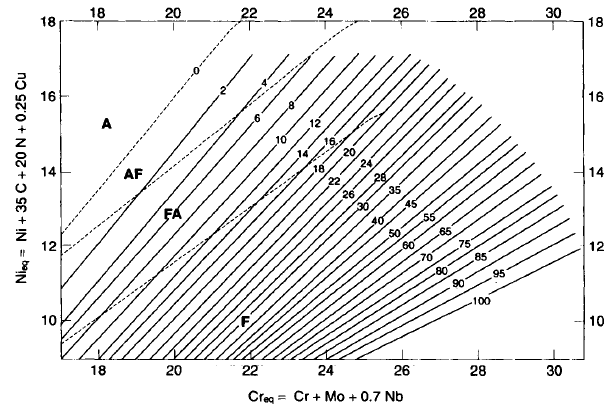
\includegraphics[width=1\textwidth]{rys.2.WRC.Kotecki.png}
    \caption{Diagram WRC-1992 (Kotecki \& Siewert, 1992)}
    \label{fig:mesh2}
\end{figure}

\noindent Równania na  $Cr_{eq}$ i~$Ni_{eq}$ są następujące (zgodnie z~rys. \ref{fig:mesh2}):
\begin{equation}
\label{eq1}
	Cr_{eq} = Cr + Mo + 0.7Nb
\end{equation}
\begin{equation}
\label{eq2}
	Ni_{eq} = Ni+35C+20N+0.25Cu
\end{equation}
gdzie symbole pierwiastków przedstawiają procent wagi każdego pierwiastka.
W kolejnej pracy \cite{Vitek03.I} dotyczącej predykcji FN ci sami autorzy wykorzystali sieć neuronową, która na wejściu przyjmowała procent wagowy $13$ pierwiastków ($Fe, Cr, Ni, C, N, Mo, Mn, Si, Cu, Ti, Nb, V~$i$~Co$), czyli warstwa z~$13$ neuronami, następnie warstwa ukryta z~sześcioma neuronami, natomiast na wyjściu był pojedynczy neuron, który zwracał liczbę ferrytową (rys. \ref{fig:mesh3}).

\begin{figure}[h]
    \centering
    
\includegraphics[width=1\textwidth]{rys.3.ORFN.Vitek.2003.png}
    \caption{Model sieci neuronowej ORFN (Vitek, 2003)}
    \label{fig:mesh3}
\end{figure}

Wyniki zostały przedstawione w~\cite{Vitek03.II} i~jak się okazało, testowana sieć zwracała lepsze wyniki od jakichkolwiek dotychczasowych podejść z~błędem RMS mniejszym o~$50\%$ od poprzedniej najlepszej metody. 
    W~ostatnim przytoczonym artykule dotyczącym predykcji FN \cite{Vasudevan13} również zastosowano sieć neuronową, a~konkretnie bayesowską sieć neuronową (BNN). Na wejściu mamy taką samą warstwę, jak w~poprzedniej pracy, natomiast tutaj jest więcej neuronów w~warstwie ukrytej. Poprawa wyników względem poprzedniej pracy wynosi około $15\%$ (błąd RMS) testując na niezależnym zbiorze danych nieużywanych w~szkoleniu.

\subsection{Predykcja własności mechanicznych odlewów}
\label{sub:predykcja.1}

Początki rozwoju i~przetwarzania materiałów nie były łatwe. Mimo wielu przeprowadzonych badań naukowych nad materiałami wciąż pozostaje wiele problemów, w~przypadku których brakuje metod ilościowych. Tyczy się to głównie predykcji takich parametrów konstrukcyjnych jak wytrzymałość na rozciąganie, trwałość, twardość itp. Pierwsze badania dotyczące własności mechanicznych odlewów przyjmujące podejście ilościowe brały pod uwagę szczegółowy skład chemiczny oraz takie parametry jak rekrystalizacja, proces starzenia, zakres pracy na zimno, temperatura badania czy szybkość odkształcania \cite{Bhadeshia07, Badmos13}. W~obydwu tych pracach zastosowano sieci neuronowe oraz uzasadniono, że modele matematyczne sobie nie radzą z~wymienionymi wyżej parametrami. Standardowo zastosowano sieć, w~której na wejściu podawano procent wagowy pierwiastków w~badanym materiale. 

Jedną z~głównych własności mechanicznych jest wytrzymałość na rozciąganie (ang. \textit{ultimate tensile strength}, UTS), która jest badana od wielu lat. Po fazie odlewu inżynierowie wykorzystują w~swoich obliczeniach tę i~inne wartości w~celu obliczenia odkształcania się, funkcji przyłożonego obciążenia, czasu i~wiele innych. Jest ona jednym z~ważniejszych czynników do uwzględnienia, gdyż niewystarczająca wartość wytrzymałości może mieć fatalne skutki (jak np. zawalenie się konstrukcji). Innym powodem może być to, iż jedynym sposobem na zbadabie wartości wytrzymałości jest przeprowadzenie badań niszczących, co powoduje wzrost kosztów produkcji \cite{Santos09}. Jednym ze sposobów analizy wartości UTS jest predykcja za pomocą wartości różnych właściwości odlewu. W~przywołanej wcześniej pracy \cite{Santos09} oraz \cite{Nieves09} są to skład chemiczny, rozmiar odlewu, prędkość chłodzenia, obróbka termiczna. Mając dane w~postaci wartości rozdzielonych przecinkiem (CSV, od ang. \textit{comma-separated values}) można skorzystać z~klasycznych metod klasyfikacji statystycznej, jak klasyfikacja liniowa, $k$ najbliższych sąsiadów, drzewa decyzyjne czy sieci bayesowskie \cite{wiki:klas.stat}. W~przytoczonej pracy skupiono się na sieciach bayesowskich. Wyniki są optymistyczne: dokładność na poziomie ponad 82\% oraz błędy MAE (średni błąd bezwzględny, od ang. \textit{mean absolute error}) oraz średni błąd kwadratowy (MSE, od ang. \textit{mean square error}) na poziomie odpowiednio $0.2$ oraz $0.35$. Inne przetestowane metody w~tym artykule to $k$ najbliższych sąsiadów (KNN, od ang. \textit{k-Nearest Neighbors}) oraz sztuczne sieci neuronowe (ANN, od ang. \textit{artificial neural networks}), które osiągnęły podobne, aczkolwiek nieco gorsze wyniki. 
Wytrzymałość na rozciąganie można przewidywać na podstawie dwóch różnych źródeł danych wejściowych \cite{Yang16}:
\begin{itemize}
\item
skład chemiczny metalu oraz zmienne procesu walcowania, jak temperatura, czy przebieg;
\item
dane na temat mikrostruktury. 
\end{itemize} 

\noindent W~pracy tej jako dane wejściowe wykorzystano skład chemiczny, specyfikacje geometryczne oraz zmienne dotyczące procesu rolowania, natomiast modelem użytym do predykcji wartości wytrzymałości na rozciąganie była ponownie bayesowska sieć neuronowa. Sieć ta składała się z~jednej warstwy ukrytej, która z~kolei składała się z~siedmiu neuronów. Jak stwierdzają autorzy, sieć BNN lepiej się sprawdza w~tym celu od tradycyjnych sieci neuronowych, a~to ze względu na wyższą odporność na nadmierne dopasowanie (ang. \textit{overfitting}), szczególnie w~przypadku, gdy ilość danych jest znacznie ograniczona i~nie mamy możliwości zgromadzenia dużej ilości wysokiej jakości danych.
    
Bardzo podobne podejście zastosowano w~pracy \cite{Wang20}, gdzie użyto sieci neuronowej, a~na jej wejściu podawano 20 zmiennych, takich jak skład chemiczny, warunki obróbki cieplnej czy temperatura badania. W~ten sposób uzyskano $93\%$ wartości współczynnika R-kwadrat dla granicy plastyczności (YS, od ang. \textit{yield strength}) oraz UTS.

\subsection{Predykcja błędów w~produkcji odlewniczej}
\label{sub:predykcja.2}

Innym, ciekawym podejściem jest to zaprezentowane w~pracy Penya et al. \cite{Yoseba08}, a~mianowicie ponownie zostały wykorzystane bayesowskie sieci neuronowe, lecz tym razem w~celu predykcji obecności mikrouszkodzeń w~odlewie przed lub w~trakcie procesu odlewnictwa. Dzięki takim danym można wpłynąć na proces odlewniczy w~taki sposób, aby zredukować liczbę defektów. W~sieci BNN wykorzystano na wejściu osiem zmiennych takich jak cechy geometryczne (dwie zmienne), jakość metalurgiczna (trzy zmienne), jakość formy (jedna zmienna) oraz dwie zmienne dotyczące samego procesu. Wyniki są obiecujące, gdyż dzięki temu podejściu udało się zredukować liczbę defektów z~$5\%$ do $0.075\%$ w~przypadku pierwszej odlewni oraz z~$4.7\%$ do $0.19\%$ w~przypadku drugiej odlewni.

\section{Powiązane prace – stan aktualny}
\label{sec:stan.aktualny}

\subsection{Predykcja cech i~jakości odlewów za pomocą metod rozpoznawania obrazów}
\label{sub:predykcja.3}

Wewnętrzna struktura materiału nazywana jest mikrostrukturą. Określa ona wszystkie jego właściwości fizyczne i~chemiczne. Pomimo tego, że charakterystyka mikrostrukturalna jest szeroko rozpowszechniona i~dobrze znana, klasyfikacja mikrostrukturalna jest zazwyczaj przeprowadzana „ręcznie” przez ekspertów. Ze względu na złożoność mikrostruktur (mogą się one składać z~podstruktur) ich klasyfikacja jest bardzo trudna i~dotychczas nie powstało zbyt wiele prac naukowych podejmujących się próby klasyfikacji mikrostruktur. Wcześniejsze artykuły zazwyczaj oddzielały fazę klasyfikacji mikrostruktur od fazy ekstrakcji cech \cite{Azimi18}. Dzięki postępowi metod głębokiego uczenia (ang. \textit{deep learning}, DL) otworzyły się nowe możliwości. Wiele metod głębokiego uczenia w~różnych zadaniach zwraca najlepsze wyniki, jakie udało się dotychczas uzyskać, dlatego warto się nad tymi metodami pochylić. 

W pierwszej przytoczonej tutaj pracy opracowano nową zautomatyzowaną metodę wykorzystującą dyfrakcję wstecznie rozproszonych elektronów (EBSD, od ang. \textit{electron backscatter diffraction}), aby skutecznie identyfikować i~określać ilościowo mikroskładniki ferrytowe w~złożonych mikrostrukturach różnych gatunków stali \cite{Shrestha13}. Identyfikowano rodzaj ferrytu dla każdego ziarna, co wiązało się z~powiązaną z~nimi wielkością ziaren. Różne odmiany ferrytów mają różne profile dezorientacji na granicach ziaren, aczkolwiek jest ona zależna od kąta, toteż zostało to wykorzystane w~badaniach.

Z~kolei w~pracy \cite{Britz17} zastosowano korelacyjne podejście oparte na EBSD i~mikroskopii optyczno-świetlnej (LOM, od ang. \textit{light-optical microscopy}), zamiast niezależnie korzystać z~powszechnych metod. Wykorzystując rozkład orientacji ziarna w~EBSD, ręcznie ustalono progi przy pomocy próbki referencyjnej tej samej płytki z~mikrostrukturą. Podobnie, w~przypadku LOM, próg był ręcznie ustalany i~mógł być zweryfikowany krzyżowo.

Kolejna przeanalizowana praca \cite{Azimi18} dotyczy klasyfikacji mikrostrukturalnej składników stali niskowęglowej za pomocą metod głębokiego uczenia. Takie podejście może być pomocne przy ocenie jakości danego odlewu jak i~predykcji jego właściwości mechanicznych. W~artykule wykorzystano w~pełni splotową sieć neuronową (ang. \textit{Fully Convolutional Neural Network}, FCNN), na której wejście podawano segmentowane piksele. System ten osiągnął niemal $94\%$ skuteczność, tym samym przewyższając najlepszą dotychczas metodę. Jak stwierdzają autorzy, nie tylko wynik jest doskonały sam w~sobie, ale również wyznacza linię dla przyszłych badań, m.in. związanych z~oceną jakości stali (i nie tylko). W~pracy tej, oprócz wspomnianego modelu, przetestowano również szereg innych metod oraz podejść. Jednym z~zastosowanych podziałów klasyfikacji jest klasyfikacja mikrostruktur oparta na obiekcie (ang. \textit{object-based microstructural classification}). Polega ona na wycinaniu obiektów z~obrazów, a~następnie klasyfikacji wyciętych kształtów do jednej z~kilku klas (ferryt, cementyt, austenit, perlit, bainit, martenzyt), jak pokazano na rysunku \ref{fig:mesh4}.  

\begin{figure}[h]
    \centering
    
\includegraphics[width=1\textwidth]{rys.4.VGG.schema.png}
    \caption{Klasyfikacja oparta na obiektach przy użyciu CNN. Obiekty są wycinane z~obrazów a~następnie klasyfikowane przez wytrenowane CNN (VGG16). Rozmiar wejściowy jest z~góry określony (Azimi et al., 2018)}
    \label{fig:mesh4}
\end{figure}

\noindent Jednakże, jak zauważono w~pracy, podejście to ma jedną wielką wadę, a~mianowicie konieczna jest zmiana rozmiarów wycinanych kształtów tak, aby odpowiadała wejściu sieci neuronowej, które jest z~góry ustalone (224 na 224 pikseli). W~ten sposób możemy zniszczyć cenne dane związane np. z~teksturą. Po przeprowadzeniu testów, przy użyciu tego podejścia uzyskano wynik na poziomie 49\% dokładności (który był dotychczas najlepszy). Drugie podejście, jakie zostało przetestowane w~\cite{Azimi18} polega na klasyfikacji pod względem pikseli (rys. \ref{fig:mesh5}). Na wejście sieci są podawane obrazki, które otrzymujemy poprzez wycinanie kawałków oryginalnych obrazów metodą przesuwnego okna. Wykonujemy tę operację tyle razy, aby pokryć cały obraz wejściowy. Wyjściem takiej sieci jest macierz 3D z~liczbą kanałów równą liczbie klas. Każdy piksel tej macierzy posiada wartość reprezentującą ufność (bądź prawdopodobieństwo) przynależności do danej klasy mikrostruktury. Następnie przeprowadzany jest etap klasyfikacji według pikseli, wybierając klasę z~najwyższym prawdopodobieństwem (pewnością, ufnością) dla każdego piksela. Następnie wszystkie segmenty należące do oryginalnego obrazu wejściowego są scalane razem (rys. \ref{fig:mesh5}). Wtedy do każdego obiektu stosowana jest zasada maksymalnego głosowania i~przypisywana jest mu klasa, jaką posiada większość pikseli (tzn. obiektowi jest przypisywana klasa mikrostruktury z~maksymalną liczbą sklasyfikowanych pikseli wewnątrz obiektu). W~pracy zastosowano również równoważenie klas oraz rozszerzenie danych (ang. \textit{data augmentation}). Równoważenie klas było konieczne, ponieważ występowały duże rozbieżności pomiędzy liczebnością przykładów w~różnych klasach, natomiast oryginalne było samo podejście do tego tematu, a~mianowicie w~zależności od liczności klasy stosowano różne rozmiary kroku (ang. \textit{stride}), tak, aby uzyskać mniejszą lub większą liczbę wyciętych przykładów. Natomiast rozszerzenie danych odbyło się poprzez rotację obrazków o~90°, 180° oraz 270°, dzięki czemu zbiór obrazków został rozszerzony aż czterokrotnie. Pomimo iż sama augmentacja nie miała znaczącego wpływu na wyniki, to dzięki niej uzyskano wzrost o~2 punkty procentowe.
\begin{figure}[h]
    \centering
    
\includegraphics[width=1\textwidth]{rys.5.segmentacja.jpg}
    \caption{Klasyfikacja mikrostrukturalna oparta na segmentacji z~maksymalną liczbą głosów. Obraz wejściowy jest przycinany, wycinki są przekazywane do sieci FCNN. Następnie segmentowane wycinki są zszywane razem. W~ostatnim kroku stosowane jest głosowanie dla wynikowego zszytego obrazu (Azimi et al., 2018)}
    \label{fig:mesh5}
\end{figure}
Dzięki takiemu podejściu udało się poprawić najlepszy dotychczas wynik aż o~45 punktów procentowych~(sic!). Wyniki wszystkich przetestowanych metod zostały przedstawione w~tab. \ref{tab:tab1}.

\begin{table}[h]
	\centering
	\begin{threeparttable}
		\caption{Wyniki klasyfikacji mikrostrukturalnej przy użyciu metod opartych na obiektach oraz opartych na pikselach (Azimi et al., 2018)}
		\label{tab:tab1}
		\begin{tabularx}{1\textwidth}{ |X|X|X|X| }
  \hline
   \textbf{Metoda} & \textbf{Typ} & \textbf{Strategia treningu} & \textbf{Dokładność}\\
  \hline
  Pauly et al. \cite{Pauly16} & oparte na obiektach & — & 48.89\%\\
  \hline
  CIFAR-Net & oparte na obiektach & od zera (ang. \textit{from scratch}) & 57.03\%\\
  \hline
  VGG19 + SVM & oparte na obiektach & — & 64.84\%\\
  \hline
  VGG16 & oparte na obiektach & strojenie (ang. \textit{fine tuning}) & 66.50\%\\
  \hline
  MVFCNN\tnote{a} & oparte na pikselach & strojenie (ang. \textit{fine tuning} & \textbf{93.94\%}\\
  \hline
\end{tabularx}
		\begin{tablenotes}
			\footnotesize
			\item[a] Metoda MVFCNN to metoda badana w~przytoczonym artykule \cite{Azimi18}. Wynik ten został osiągnięty na obrazkach otrzymanych metodą skaningowej mikroskopii elektronowej (SEM, od ang. \textit{scanning-electron microscopy}), natomiast na obrazkach metodą LOM osiągnięto wynik zaledwie około 70\%\textellipsis
		\end{tablenotes}
	\end{threeparttable}
\end{table}

Kolejną pracą, z~obiecującymi wynikami, która również korzysta z~uczenia głębokiego, jest \cite{Durmaz21}. Celem owej pracy jest segmentacja struktur w~stali o~złożonej fazie. Autorzy zastosowali w~niej sieci Vanilla U-Net oraz U-Net VGG16, uzyskując najlepsze wyniki skuteczności odpowiednio $91.6\%$ oraz $90.6\%$. Rezultaty te otrzymano dla danych w~postaci obrazów uzyskanych metodą LOM. Wykorzystano również dane w~postaci obrazów otrzymywanych metodą SEM, lecz skuteczności były mniejsze o~około $10$ punktów procentowych.

\section{Wnioski}
\label{cha2.3}

Jak widzimy, dziedzina, jaką jest inżynieria materiałowa, mimo iż rozwijana już od wielu lat, nadal wymaga wiele pracy, która usprawni proces wytwarzania materiałów, a~także zaoszczędzi środki, które obecnie są marnowane na badania niszczące. Właściwości materiału takie jak wytrzymałość, wiązkość, twardość, kruchość lub ciągliwość są istotne przy kategoryzacji materiału lub komponentu według ich jakości, lecz testy te są zwyczajowo drogie. Dlatego metody uczenia maszynowego są uznawane za pomocne w~przewidywaniu właściwości odlewów \cite{Stoll21}. Z~drugiej strony problemem może być wciąż niewystarczająca ilość danych uczących –  co można zauważyć po tym, iż nie udało się znaleźć żadnych publicznie udostępnionych danych w~postaci zdjęć, które można byłoby dołączyć do własnego zbioru danych. Z~tego też względu przeprowadzone testy będą się opierały głównie na klasyfikacji metalu ze względu na wysoką bądź niską odporność na rozciąganie, a~także ze względu na wysoką bądź niską granicę sprężystości, gdyż takimi właśnie danymi dysponujemy.

Początkowo w~celu predykcji właściwości mechanicznych korzystano z~dosyć prymitywnych rozwiązań jak np. odczytywanie z~wykresu właściwości za pomocą samego składu chemicznego. Następnie, po wielu latach rozwoju w~dziedzinie materiałoznawstwa, jak i~informatyki i~uczenia maszynowego zaczęto korzystać z~takich zmiennych jak skład chemiczny, wielkość odlewu, prędkość chłodzenia czy proces obróbki termicznej wykorzystując takie modele, jak sieci bayesowskie, algorytm k-nn czy sieci neuronowe. Z~czasem sieci neuronowe zaczęły osiągać najlepsze wyniki, w~tym momencie znacznie zostawiając w~tyle pozostałe metody. A~więc co do wykrywania właściwości mając wspomniane wcześniej dane, sieci neuronowe zostały dosyć dobrze przetestowane i~dają gwarantowane, wysokie wyniki. Co natomiast z~danymi w~postaci obrazów? Tutaj widzimy, że powoli również są adaptowane sieci neuronowe, a~w~szczególności głębokie sieci neuronowe \cite{Azimi18, Pauly16}, które dają nadzwyczaj obiecujące wyniki. Natomiast prace te były związane z~wykrywaniem pojedynczych struktur na obrazkach, a~nie z~predykcją samych właściwości mechanicznych. Wykorzystano w~nich tzw. semantyczną segmentację obrazu, która wydaje się najbardziej optymistyczna, aczkolwiek nie posiadamy takich danych. Jednak jak najbardziej można to uznać za obiecujący kierunek poszukiwań w~celu zwiększenia skuteczności sieci wykrywających i~klasyfikujących struktury na obrazkach.

Podsumowując, sieci neuronowe udowodniły swoją przydatność w~zakresie predykcji zawartości ferrytu w~składzie chemicznym spoiny czy predykcji właściwości mechanicznych za pomocą składu chemicznego i~danych dotyczących samego procesu wyrobu takiego materiału. Znaczące postępy też są widoczne w~obszarze klasyfikacji struktur na obrazie. Jednak nadal brakuje badań w~obszarze predykcji właściwości mechanicznych z~obrazów, dlatego autor niniejszej pracy podjął się próby przeprowadzenia takich testów i~przeanalizowania możliwości sieci neuronowych (w szczególności głębokich sieci neuronowych) w~tym zakresie. Dysponując oznakowanymi danymi w~postaci obrazków, które zostały podzielone na dwa podzbiory –  ze względu na odporność na rozciąganie oraz ze względu na granicę sprężystości, warto przetestować możliwości predykcyjne sieci neuronowych dla tak postawionego problemu. Dodatkowo można skorzystać z~pomysłów (przedstawionych w~powyższych podrozdziałach) dotyczących klasyfikacji struktur na obrazach, aby mieć dodatkowe informacje, które być może będą pomocne w~docelowej klasyfikacji. Oprócz tego, jako inne źródła informacji można z~obrazów wyciągać momenty, które zostały opracowane wiele lat temu i~dotychczas były wykorzystywane z~sukcesami. Ponadto, głównie jako odniesienie, można wykorzystać klasyczne klasyfikatory typu las losowy, maszyna wektorów nośnych czy inne. Oczekuje się wyników na poziomie zbliżonym do wyników przedstawionych w~powyższych pracach, które korzystały z~sieci neuronowych dla danych zawierających m.in. skład chemiczny.  








%\chapter{Przykłady elementów pracy dyplomowej}
%
%\section{Liczba}
%
%Pakiet \texttt{siunitx} zadba o to, by liczba została poprawnie sformatowana: \\
%\begin{center}
%	\num{1234567890.0987654321}
%\end{center}
%
%
%\section{Rysunek}
%
%Pakiet \texttt{subcaption} pozwala na umieszczanie w podpisie rysunku odnośników do ,,podilustracji'': \\
%
%\begin{figure}[h]
%	\centering
%	\begin{subfigure}{0.35\textwidth}
%		\centering
%		\framebox[2.0\width]{A}
%		\subcaption{\label{subfigure_a}}
%	\end{subfigure}
%	\begin{subfigure}{0.35\textwidth}
%		\centering
%		\framebox[2.0\width]{B}
%		\subcaption{\label{subfigure_b}}
%	\end{subfigure}
%	
%	\caption{\label{fig:subcaption_example}Przykład użycia \texttt{\textbackslash subcaption}: \protect\subref{subfigure_a} litera A, \protect\subref{subfigure_b} litera B.}
%\end{figure}
%
%\section{Tabela}
%
%Pakiet \texttt{threeparttable} umożliwia dodanie do tabeli adnotacji: \\
%
%\begin{table}[h]
%	\centering
%	
%	\begin{threeparttable}
%		\caption{Przykład tabeli}
%		\label{tab:table_example}
%		
%		\begin{tabularx}{0.6\textwidth}{C{1}}
%			\toprule
%			\thead{Nagłówek\tnote{a}} \\
%			\midrule
%			Tekst 1 \\
%			Tekst 2 \\
%			\bottomrule
%		\end{tabularx}
%		
%		\begin{tablenotes}
%			\footnotesize
%			\item[a] Jakiś komentarz\textellipsis
%		\end{tablenotes}
%		
%	\end{threeparttable}
%\end{table}
%
%\section{Wzory matematyczne}
%
%Czasem zachodzi potrzeba wytłumaczenia znaczenia symboli użytych w równaniu. Można to zrobić z użyciem zdefiniowanego na potrzeby niniejszej klasy środowiska \texttt{eqwhere}.
%
%\begin{equation}
%E = mc^2
%\end{equation}
%gdzie
%\begin{eqwhere}[2cm]
%	\item[$m$] masa
%	\item[$c$] prędkość światła w próżni
%\end{eqwhere}
%
%Odległość półpauzy od lewego marginesu należy dobrać pod kątem najdłuższego symbolu (bądź listy symboli) poprzez odpowiednie ustawienie parametru tego środowiska (domyślnie: 2 cm).

\chapter{Uczenie maszynowej}
\label{cha:cha3}

Uczenie maszynowe (ML, od ang. machine learning) to nauka o algorytmach komputerowych, które automatycznie ulepszają się dzięki doświadczeniu i wykorzystaniu danych [22]. Algorytmy uczenia maszynowego są budowane na podstawie przykładowych danych, zwanych „danymi szkoleniowymi”, w celu prognozowania lub podejmowania decyzji bez bezpośredniego zaprogramowania do tego [23]. Natomiast nieco bardziej techniczną definicję uczenia maszynowego przedstawił Tom Mitchell w 1997 roku: Mówimy, że program komputerowy uczy się na podstawie doświadczenia E w odniesieniu do jakiegoś zadania T i pewnej miary wydajności P, jeśli jego wydajność (mierzona przez P) wobec zadania T wzrasta wraz z nabywaniem doświadczenia E.
    Dyscyplina uczenia maszynowego wykorzystuje różne podejścia do uczenia modeli wykonywania zadań, w przypadku których nie jest dostępny w pełni zadowalający algorytm. Wstęp do uczenia maszynowego wraz z wyjaśnieniem pojęć podstawowych został przedstawiony w rozdziale 3.1. Główne nurty zostały zaprezentowane w rozdziale 3.2.

\section{Pojęcia podstawowe}
\label{cha:cha3.1}

Jednym z podstawowych terminów w uczeniu maszynowym jest atrybut (ang. attribute). Oznacza on konkretny typ danych (np. wiek). Innym terminem jest cecha (ang. feature), która oznacza atrybut wraz z jego wartością. Mają one zastosowanie między innymi w przypadku danych w postaci plików csv. Aby móc skorzystać z mocy uczenia maszynowego, musimy wybrać jakiś model, który wytrenujemy. Modele zostały opisane w rozdziale 3.6., natomiast ogólne typy uczenia maszynowego w rozdziale 3.2. Jednakże, zanim ostatecznie zdecydujemy się który model powinien być wykorzystany, należy porównać istniejące modele. W tym celu zazwyczaj wykorzystuje się funkcję kosztu, która mówi nam jak duży błąd popełnia model podczas predykcji [32]. 
    Innym aspektem związanym z modelami uczenia maszynowego jest to, jakie wyniki osiąga dany model (również względem posiadanych danych). Jednym z problemów z tym związanych jest tzw. przetrenowanie, bądź też inaczej, nadmierne dopasowanie (ang. overfitting). Oznacza to, iż model bardzo dobrze sobie radzi na danych uczących, natomiast dla danych testowych wyniki są już o wiele gorsze. Jest to równoznaczne z tym, iż model nie uogólnia danych zbyt dobrze. Zdarza się to najczęściej, gdy mamy zbyt małą ilość danych i dodatkowo użyjemy zbyt skomplikowanego modelu. Jest to dosyć znany problem, który występuje w literaturze pod nazwą kompromis między obciążeniem a wariancją (ang. bias-variance tradeoff). Istnieje wiele rozwiązań, które zapobiegają przetrenowaniu. Jednym z nich jest regularyzacja. To, jak bardzo chcemy regularyzować proces uczenia zależy od tego, jakie wartości przypiszemy hiperparametrom (ang. hyperparameters). 
Analogicznym problemem jest niedotrenowanie (ang. underfitting), jednakże w tym przypadku chodzi o dokładnie przeciwne zjawisko, tzn. gdy model jest zbyt prosty (w stosunku do danych). W tym przypadku istnieje kilka rozwiązań, jak [32]:
wybór mocniejszego modelu (który posiada większą liczbę parametrów),
zmodyfikowanie danych w taki sposób, aby posiadały większą liczbę cech (patrz rozdział 3.3.: inżynieria cech),
redukcja regularyzacji (bądź innych ograniczeń modelu).
    Kolejnym problemem związanym ze słabymi wynikami modelu jest aspekt dotyczący danych. Pierwsze utrudnienie to zbyt mała liczba danych. W zależności od zagadnienia wymagana liczba przykładów uczących może się wahać między setkami (np. predykcja obecności choroby u pacjenta na podstawie danych zdrowotnych) a milionami (np. rozpoznawanie mowy, klasyfikacja tekstu). Kolejnym problemem związanym z danymi jest zaszumienie danych. Innymi słowy, mamy z taką sytuacją do czynienia, gdy dane nie odzwierciedlają rzeczywistości (a przynajmniej nie całkowicie poprawnie). Wtedy, niezależnie od zastosowanego modelu nie ma możliwości, aby system, mając do dyspozycji niereprezentatywne dane, radził sobie dobrze na danych testowych. Dotyczy to również przypadków, gdy dane są błędne. Rozwiązaniem tego problemu może być przykładowo [32]:
odrzucenie elementów odstających,
odrzucenie, bądź uzupełnienie brakujących danych,
rozpoznanie i odrzucenie błędnych danych.
Ostatnim poruszonym problemem związanym z danymi są nieistotne cechy. Mogą one działać jak szum i obniżać jakość posiadanych danych. W tym przypadku rozwiązaniem może być odrzucenie nadmiarowych cech i uproszczenie danych. Kwestia ta zazwyczaj jest poruszana w trakcie wykonywania inżynierii cech (patrz rozdział 3.3.).
Gdy już posiadamy wyuczony model, dobrze byłoby upewnić się, iż działa on tak, jak powinien. Podejście, które się utrwaliło jest podział posiadanych danych na zbiory danych uczących oraz danych testowych (czasami również odkłada się jeszcze jeden zbiór danych walidacyjnych, aby we wczesnej fazie wyszukiwania odpowiedniego modelu sprawdzać wyniki właśnie na tych danych, a po wybraniu ostatecznego modelu, przetestować jego skuteczność na danych testowych). Zazwyczaj 80\% wszystkich danych przeznacza się na dane uczące [32].
Docelowym zadaniem, które będzie badane w tej pracy jest klasyfikacja wytrzymałości odlewów na podstawie mikrostruktur. Dane, jakimi dysponujemy posiadają dwie etykiety: niska oraz wysoka wytrzymałość (bądź też inny wskaźnik). A więc trzeba będzie skorzystać z klasyfikatora binarnego. Jak natomiast zweryfikować jak dobrze sobie radzi dany klasyfikator? Aby to stwierdzić w statystyce używa się wielu miar, które pokrótce zostaną tutaj przedstawione. Zacznijmy od wyjaśnienia takiego pojęcia jak tablica pomyłek. W klasyfikacji binarnej dane są oznaczone dwiema etykietami, dla uproszczenia nazwijmy je pozytywną i negatywną. Podczas klasyfikacji są im przypisywane przewidywane etykiety i istnieje możliwość, że etykieta zostanie źle przypisana. Ilustruje to poniższa tabela (tab. 2).

\begin{table}[h]
	\centering
	
	\begin{threeparttable}
		\caption{Schemat tablicy pomyłek (wikipedia)}
		\label{tab:tab2}
				
		\begin{tabularx}{1\textwidth}{ |c|c|X|X| }\hline
		  \multicolumn{2}{|c|}{\multirow{2}{*}{}} & \multicolumn{2}{|c|}{\textbf{Klasa rzeczywista}}\\ \cline{3-4}
      
		  \multicolumn{2}{|c|}{} & \multicolumn{1}{|c|}{\textbf{pozytywna}} & \multicolumn{1}{c|}{\textbf{negatywna}}\\ \hline
       
		  \multirow{2}{*}{\textbf{Klasa predykowana}} & \textbf{pozytywna} & prawdziwie pozytywna (TP) & fałszywie pozytywna (FP)\\ \cline{2-4}
      
		   & \textbf{negatywna} & fałszywie negatywna (FN) & prawdziwie negatywna (TN)\\ \hline
		\end{tabularx}

	\end{threeparttable}
\end{table}

Następnie, w celu ułatwienia oceny klasyfikatora, można wprowadzić poniższe miary wydajności [32, 33]:
- prawdziwie pozytywna (ang. true positive, TP),
- prawdziwie negatywna (ang. true negative, TN),
- fałszywie pozytywna (ang. false positive, FP), tzw. błąd pierwszego rodzaju
- fałszywie negatywna (ang. false negative, FN), tzw. błąd drugiego rodzaju
Są to podstawowe miary wydajności za pomocą których dalej zdefiniujemy bardziej rozbudowane miary. Ale wracając do tablicy pomyłek, pożądanym wynikiem jest uzyskanie wysokich liczb na głównej przekątnej tablicy pomyłek (czyli prawdziwie pozytywna oraz prawdziwie negatywna), natomiast jak najmniejsze (najlepiej zerowe) wartości na pozostałej przekątnej. Dzięki tej macierzy możemy przeanalizować w jakich przypadkach nasz klasyfikator myli się najczęściej. Dalej można wprowadzić bardziej zwięzłe metryki [32]:
- dokładność (ang. accuracy, ACC)
\begin{equation}
ACC=\frac {TP+TN} {TP+FP+FN+TN}
\end{equation}
%Wzór na dokładność (ang. accuracy, ACC)

- precyzja (ang. precision, PPV)
\begin{equation}
PPV=\frac {TP} {TP+FP}
\end{equation}
%Wzór na precyzję

- czułość (ang recall, TPR)
\begin{equation}
TPR=\frac {TP} {TP+FN}
\end{equation}
%Wzór na czułosć

Dokładność mówi nam jaki odsetek predykcji stanowią poprawne predykcje (patrz wzór 3). Kolejną miarą jest precyzja, która mówi nam jaka jest dokładność pozytywnych prognoz (4). Ostatnią przedstawioną tutaj miarą jest czułość i jest to odsetek pozytywnych przykładów, które zostały poprawnie zaklasyfikowane (5). Macierz pomyłek można również rozszerzyć do klasyfikacji wieloklasowej, co zostało uczynione w badaniach (rozdział 5). Bardziej zaawansowane pojęcia i metody będą wyjaśniane w dalszych rozdziałach niniejszej pracy (w miejscu ich zastosowania).

\section{Typy uczenia maszynowego}
\label{cha:cha3.2}

Jednym z kryterium podziału systemów uczenia maszynowego może być stopień i rodzaj nadzorowania procesu uczenia [32]. Pod tym względem możemy wyróżnić cztery główne rodzaje, przedstawione w poniższych podrozdziałach.

\subsection{Uczenie nadzorowane}
\label{cha:cha3.2.1}

Uczenie nadzorowane (ang. supervised learning) polega na trenowaniu modelu za pomocą danych, które zostały przygotowane przez ludzkiego nadzorcę jako pary <obiekt uczący; etykieta>[24]. Celem takiego systemu jest nauczenie się przewidywania prawidłowej odpowiedzi dla danego obiektu wejściowego oraz generalizacja na przypadki, które nie są obecne w danych uczących [24]. 
Uczenie nadzorowane można podzielić na klasyfikację oraz regresję, co jest determinowane przez etykietę danych. W przypadku, gdy każda etykieta należy do skończonego zbioru, mówimy o klasyfikacji. Jeżeli zaś etykiety mogą przyjmować np. dowolną wartość liczby rzeczywistej, wtedy mówimy o regresji. Jedne z ważniejszych przykładowych algorytmów tego rodzaju są:
regresja liniowa (ang. linear regression),
algorytm k-najbliższych sąsiadów (ang. k-nearest neighbors algorithm),
regresja logistyczna (ang. logistic regression),
drzewa decyzyjne (ang. decision tree),
lasy losowe (ang. random decision forest),
maszyny wektorów nośnych (ang. support-vector machine),
sieci neuronowe.
Te metody i inne zostały opisane w podrozdziale 3.6. 

\subsection{Uczenie częściowo nadzorowane}
\label{cha:cha3.2.2}

Uczenie częściowo nadzorowane (ang. semi-supervised learning) polega na trenowaniu modelu za pomocą danych zarówno oznakowanych, jak i nieoznakowanych. Wykorzystuje się go wtedy, gdy liczba danych jest ogromna i system sam może zaproponować odpowiedzi. Często algorytmy tego rodzaju stanowią kombinację algorytmów uczenia nadzorowanego i nienadzorowanego [32].

\subsection{Uczenie nienadzorowane}
\label{cha:cha3.2.3}

Uczenie nienadzorowane (ang. unsupervised learning) polega na wykrywaniu wzorców, relacji na podstawie nieoznaczonych danych, możliwie maksymalnie bez ingerencji człowieka. Im większa liczba danych, tym bardziej precyzyjne wyniki. Jedne z ważniejszych algorytmów uczenia nienadzorowanego, to:
metoda k-średnich (ang. k-means clustering),
analiza głównych składowych (ang. principal component analysis, PCA),
stochastyczne osadzanie sąsiadów przy użyciu rozkładu t (ang. t-distributed stochastic neighbor embedding, t-SNE).
Jednym z przykładów użycia uczenia nienadzorowanego może być wizualizacja danych, m.in. przy pomocy algorytmów PCA bądź t-SNE. Ten typ uczenia maszynowego nie został wykorzystany w niniejszej pracy, dlatego nie będzie głębiej analizowany.

\subsection{Uczenie przez wzmacnianie}
\label{cha:cha3.2.4}

Uczenie przez wzmacnianie (ang. reinforcement learning, RL) polega na interakcji ze środowiskiem za pomocą polityki, mając do dyspozycji zestaw dozwolonych akcji (działań). Model dokonuje analizy środowiska i automatycznie zbiera z niego dane. Celem jest maksymalizacja nagrody. W uczeniu przez wzmacnianie wyróżnia się trzy główne elementy jak środowisko, agenta oraz bufor. System uczący, czyli agent, może obserwować środowisko, na tej podstawie wykonywać pewne czynności, następnie odbierać nagrody, lub kary. W następnym zaś kroku musi nauczyć się najlepszej strategii, zwanej polityką, co prowadzi do maksymalizacji nagrody [32]. Ze względu na charakterystykę tego nurtu uczenia maszynowego jest ono często stosowanie do uczenia modeli grania w gry [24].

\section{Inżynieria cech}
\label{cha:cha3.3}

Inżynieria cech jest procesem wykorzystania wiedzy dziedzinowej w celu ekstrakcji cech z surowych danych [25]. Cecha jest własnością każdej instancji danych i jest ona wykorzystywana przez model w celu predykcji. Odpowiednio przygotowane dane zwiększają skuteczność modeli [25]. Proces tworzenia cech składa się z sześciu głównych etapów [47]:
burza mózgów – ma na celu zebranie grupy ekspertów w celu zweryfikowania danych lub ustalenia sposobu przeprowadzenia ekstrakcji cech;
wybór cech – w przypadku, gdy mamy wiele cech, możemy wybrać te, które niosą za sobą najwięcej informacji. Można tego dokonać z wykorzystaniem wiedzy dziedzinowej bądź za pomocą różnych technik wyboru podzbioru cech (np. symulowane wyżarzanie, optymalizacja za pomocą roju cząstek i.in.). Ten krok jest ważny, gdyż dzięki niemu potencjalnie uzyskamy prostszy model, a prostsze modele mają większą zdolność do generalizacji poprzez redukcję wariancji (tzw. kompromis między obciążeniem a wariancją). Inne korzyści, to:
krótszy czas treningu,
uniknięcie przekleństwa wymiarowości,
lepsza interpretowalność;
tworzenie nowych cech – możemy tworzyć nowe cechy za pomocą tych istniejących, np. za pomocą średniej arytmetycznej, minimum, czy innych statystyk. Można też wykorzystać normalizację (np. standaryzacja);
testowanie wpływu cech na model – warto zautomatyzować ten proces, aby wybrać jak taki zestaw cech, który najlepiej się sprawdza na danych treningowych;
poprawa cech w razie konieczności – dalsza modyfikacja cech wraz z obserwacją wpływu na działanie modelu;
powtórzenie powyższych czynności – powtarzamy powyższe czynności do momentu, gdy przestaniemy uzyskiwać coraz lepsze rezultaty, bądź gdy dojdziemy do wniosku, iż dane są słabej jakości, bądź dysponujemy zbyt małą ich liczbą.
Cechy mogą się różnić pod względem znaczenia. Dodatkowo odpowiednio skomponowany zbiór cech może zapobiec nadmiernemu dopasowaniu się modelu do danych uczących. 

\section{Augmentacja danych}
\label{cha:cha3.4}

Augmentacja danych to zbiór technik służących zwiększaniu ilości danych poprzez dodanie do zbioru danych zmodyfikowanych kopii istniejących danych bądź nowo utworzonych danych syntetycznych z istniejących danych [26]. Dzięki temu zabiegowi możemy zapobiec nadmiernemu dopasowaniu się modelu do danych treningowych. Jest to szczególnie przydatne kiedy nie dysponujemy zbiorem danych rzędu dziesiątek tysięcy przykładów. Ponieważ nasze dane to zdjęcia mikrostruktur, dlatego w tym rozdziale zajmiemy się tylko rozszerzaniem danych w celu klasyfikacji obrazów. Możemy wymienić kilka głównych strategii:
odwrócenie – możemy odwracać obrazy w pionie i w poziomie, zachowując przy okazji oryginalne rozmiary oryginalnego zdjęcia;
rotacja – możemy obracać obrazy o 90° w każdym kierunku, otrzymując tym samym trzy nowe obrazy. W tym przypadku natomiast otrzymane obrazy mogą mieć inne rozmiary niż oryginalny obraz, w przypadku gdy nie jest on kwadratem;
skalowanie – obraz może być przeskalowany na zewnątrz lub do wewnątrz. W przypadku skalowania na zewnątrz otrzymujemy obraz o większym rozmiarze, a więc wycinając odpowiedni obszar możemy otrzymać obraz o takim samym rozmiarze jak oryginalny obraz;
wycinanie – inną możliwością jest wycinanie losowych fragmentów z obrazu. Gdy chcemy zachować oryginalny rozmiar, trzeba jeszcze przeskalować zmodyfikowany obrazek;
translacja – polega na przesuwaniu obrazu wzdłuż osi. Działa szczególnie dobrze, gdy mamy do czynienia z obrazami, które posiadają jednolite tło;
nałożenie szumu – dzięki tej technice możemy zapobiec nadmiernemu dopasowaniu się modelu do danych. 
Wśród innych metod, które również mogą się sprawdzić, można wymienić przekształcenia geometryczne, modyfikację kolorów czy losowe wymazywanie [26]. Istnieje też wiele innych, bardziej zaawansowanych metod augmentacji danych [27]. Przykładowo można zastosować tzw. generatywne sieci współzawodniczące (GAN od ang. generative adversarial network). Mogą one m.in. zmieniać domenę obrazu, jak pokazano na rysunku 6. Inną zaawansowaną techniką jest interpolacja. Może ona zostać wykorzystana w przypadku, gdy chcemy skorzystać z translacji – możemy wtedy brakujący fragment obrazu interpolować. Przyda się również, gdy chcemy skorzystać ze skalowania do wewnątrz jednocześnie zachowując oryginalny rozmiar obrazu [27]. 

\begin{figure}[h]
    \centering
    
\includegraphics[width=1\textwidth]{rys.6.transfer.png}
    \caption{Zmiana pór roku przy użyciu CycleGAN. Żródło: https://junyanz.github.io/CycleGAN/}
    \label{fig:mesh6}
\end{figure}

\section{Uczenie się przez transfer}
\label{cha:cha3.5}

Ludzie mają wrodzoną zdolność wykorzystywania wiedzy, którą zdobyli w trakcie wykonywania innego zadania. To znaczy, wiedzę, którą zdobywamy, ucząc się pewnej rzeczy, możemy wykorzystać, wykonując inne, aczkolwiek powiązane zadanie. Im bardziej powiązane są te zadania, tym łatwiej jest nam przenieść naszą wiedzę [29]. A więc w najprostszych słowach, uczenie się przez transfer to idea wykorzystania wiedzy zdobytej w ramach jednego zadania do rozwiązywania zadań pokrewnych. W ostatnich latach uczenie się przez transfer również zaczęto stosować w uczeniu maszynowym, czy też w głębokim uczeniu [31]. W tym przypadku najczęściej polega ono na wykorzystaniu już istniejącego modelu do nowego problemu. Jakie wynikają z tego korzyści? Przede wszystkim to podejście pozwala nam na osiągnięcie zamierzonych rezultatów (np. wysoka skuteczność klasyfikacji) przy użyciu mniejszej ilości danych niż w przypadku trenowania całkowicie nowego modelu. 
Uczenie się przez transfer dobrze można zilustrować na przykładzie rozpoznawania obrazów (tym lepiej, że właśnie w tym celu wykorzystano tę metodologię w niniejszej pracy), a mianowicie sieci neuronowe w początkowych warstwach wykrywają krawędzie, w kolejnych warstwach wykrywają kształty, natomiast w ostatnich warstwach wykrywają specyficzne zależności dla danego zadania [31]. A więc w celu klasyfikacji danych obiektów można skorzystać z ogólnie znanych, dobrze wytrenowanych, na wielkich zbiorach danych, głębokich sieci neuronowych (np. VGG19) w ten sposób, że budujemy nowy model, który kopiuje początkowe warstwy wcześniej wytrenowanej sieci, a następnie przyłączamy nowe warstwy, które zostaną dotrenowane w tym konkretnym celu. Oprócz wykorzystania uczenia transferowego do klasyfikacji obrazów skutecznie stosowano to podejście również w takich zadaniach, jak klasyfikacja tekstów czy filtrowanie spamu [30]. 


\section{Wykorzystane metody uczenia maszynowego}
\label{cha:Wykorzystane metody uczenia maszynowego}

W tym rozdziale zostaną przedstawione metody uczenia maszynowego, które zostały wykorzystane w trakcie realizacji pracy. Większość z nich to algorytmy uczenia nadzorowanego ze względu na charakterystykę danych.

\subsection{Maszyna wektorów nośnych}
\label{cha:Maszyna wektorów nośnych}

Maszyna wektorów nośnych (ang. Support Vector Machine, SVM) to model nadzorowanego uczenia maszynowego, która wyznacza hiperpłaszczyznę w celu rozdzielenia przykładów należących do dwóch klas z maksymalnym marginesem [24]. SVM to potężny i wszechstronny model uczenia maszynowego, który jest w stanie przeprowadzić klasyfikację liniową, nieliniową oraz regresję [32]. Rysunek 7 przedstawia koncepcję działania SVM. Model ten mapuje przykłady uczące do punktów w przestrzeni tak, aby maksymalizować odległość między dwiema kategoriami. Następnie nowe przykłady są mapowane do tej samej przestrzeni i w zależności, po której stronie marginesu się znajdują, tak są klasyfikowane. Tak jak wspomniano wyżej, za pomocą SVM również można skutecznie przeprowadzać klasyfikację nieliniową, co jest możliwe dzięki tzw. sztuczce z funkcją jądra (ang. kernel trick). Polega ona na tym, iż dane wejściowe są niejawnie odwzorowywane do przestrzeni cech o wyższym wymiarze [34]. 

\begin{figure}[h]
    \centering
    
\includegraphics[width=1\textwidth]{rys.7.svm.png}
    \caption{Działanie SVM. H1 nie separuje klas, H2 separuje, lecz z małym marginesem, natomiast H3 separuje z maksymalnym marginesem (Źródło: wikipedia)}
    \label{fig:mesh7}
\end{figure}

Jednym z problemów, które można napotkać w trakcie korzystania z SVM jest ich czułość na skalę cech. Jednakże łatwo jest to obejść przy pomocy przeskalowania cech (np. standaryzacja). Innym problemem jest konieczność posiadania całkowicie oznaczonych danych [48]. Dodatkowo parametry tego modelu są trudne do zinterpretowania. Mimo wszystko wady te nie są zbyt uciążliwe, a nawet istnieją rozwiązania, które je obchodzą. Istnieje taki model, jak SVC (ang. support-vector clustering), który można wykorzystać w celu uczenia nienadzorowanego). Dodatkowo istnieją rozszerzenia modelu SVM, dzięki którym można wykorzystać ten model do klasyfikacji wieloklasowej. Polegają one m.in. na takich strategiach, jak rozpatrywanie danej etykiety przeciwko wszystkim pozostałym (i tak dla każdej etykiety). Algorytm SVM jest jednym z najczęściej stosowanych w przemyśle, dlatego jego efektywność zostanie przetestowana na tle innych algorytmów.

\subsection{Drzewo decyzyjne}
\label{cha:Drzewo decyzyjne}

Drzewo decyzyjne (ang. decision tree) to algorytm uczenia maszynowego stosowany w celu pozyskiwania wiedzy na podstawie przykładów [36]. Mają wiele zastosowań i służą zarówno do zadań klasyfikacji, jak i regresji. Jest to struktura, która kształtem przypomina drzewo (stąd nazwa), a każda ścieżka w tym drzewie przedstawia możliwą ścieżkę decyzyjną wraz z jej skutkami [35]. Składa się ono z węzłów (które jednocześnie oznaczają jakąś decyzję, stan) i gałęzi (wybór, możliwość). Drzewo konstruowane jest od korzenia i z każdą kolejną decyzją do podjęcia jest budowany w dół, to tzw. liści (ang. leaf), które oznaczają etykietę klasy. Istnieje wiele algorytmów generowania drzew decyzyjnych. Najbardziej znane z nich, to ID3 (Iterative Dichotomiser 3), czy też C4.5. Algorytm ID3 polega na tym, że w każdej iteracji jest wybierany niewykorzystany atrybut, który daje największy wzrost informacji (bądź np. najmniejszą miarę zanieczyszczenia), a zbiór danych jest dzielony według wartości tego atrybutu. Natomiast algorytm C4.5 jest rozszerzeniem wcześniejszego algorytmu i wprowadza takie usprawnienia, jak [37]:
obsługa atrybutów ciągłych i dyskretnych,
obsługa danych z brakującymi wartościami atrybutów,
przycinanie drzew po ich utworzeniu.

Wśród największych zalet drzew decyzyjnych wymienia się [38]:
prosty algorytm,
łatwo interpretowalne wyniki,
działają nawet dla niewielkiej liczby danych,
nie wymagają przygotowywania danych (w szczególności skalowania) [32].

Natomiast posiadają też wady, takie jak [38]:
niestabilność (niewielka zmiana danych może prowadzić do dużej zmiany struktury drzewa,
często są stosunkowo niedokładne (inne klasyfikatory zazwyczaj radzą sobie lepiej),
może wystąpić problem nadmiernego dopasowania się do danych.
Pomimo tych wad klasyfikator ten zostanie wykorzystany w badaniach, głównie ze względu właśnie na jego bardzo łatwą interpretowalność.

Jako ciekawostkę można dodać, że drzewa decyzyjne składają się na algorytm lasu losowego (ang. random forest), który zostanie omówiony w podrozdziale 3.6.3. 

\subsection{Las losowy}
\label{cha:Las losowy}

Jak zostało wspomniane wyżej, drzewa decyzyjne mogą zbyt mocno dopasować się do danych treningowych. Jednym z rozwiązań jest technika lasów losowych (ang. random forest), która polega na tworzeniu wielu drzew decyzyjnych, a następnie klasyfikacji w drodze głosowania [35], a więc jako odpowiedź jest generowana dominanta klas (klasyfikacja) lub średnia przewidywana wartość (regresja) [39]. Istnieje kilka różnych algorytmów tworzenia lasów losowych. Jednym z nich jest agregacja (ang. bagging, bootstrap aggregating). Polega on na tym, iż wielokrotnie wybiera się losowe podzbiory zestawu uczącego ze zwracaniem (ang. sampling with replacement) w celu dopasowania do każdego takiego zbioru nowego drzewa [32]. Dzięki temu podejściu zmniejsza się wariancja modelu, bez zwiększania obciążenia [49], gdyż pojedyncze drzewa decyzyjne nie są ze sobą skorelowane (dzięki uczeniu ich na różnych zbiorach danych). Następnie, w celu klasyfikacji, wszystkie pojedyncze drzewa zwracają wynik, który jest uśredniony. Dodatkowo, aby jeszcze mocniej zmniejszyć korelację między drzewami, w przypadku lasów losowych korzysta się ze zmodyfikowanego algorytmu trenowania drzewa, gdzie przy każdym kolejnym węźle jest wybierany losowy podzbiór cech. Dzięki temu, jeśli w danych występuje cecha, która jest silnym predyktorem dla zmiennej przewidywanej, jej wykorzystanie w różnych drzewach zostanie ograniczone, tym samym dalej zmniejszając korelację między nimi.
Innym podejściem jest wzmacnianie (ang. boosting) [40]. Główną różnicą między agregacją a wzmacnianiem jest to, iż w przypadku tego pierwszego każde drzewo jest uczone niezależnie od pozostałych i ten etap może być przeprowadzony równolegle. Natomiast w przypadku drugiego algorytmu uczenie pojedynczych drzew następuje sekwencyjnie i każdy kolejny klasyfikator bierze pod uwagę wyniki poprzedniego klasyfikatora. Danym błędnie sklasyfikowanym przypisuje się większą wagę, tym samym kolejne modele zwracają większą uwagę trudnym danym. Jednakże w przypadku wzmacniania klasyfikacja odbywa się nieco inaczej, gdyż tutaj również mamy wagi, które są przypisywane klasyfikatorom w trakcie uczenia – im lepszy klasyfikator, tym większe wagi otrzymuje. Dzięki zastosowaniu jednego z tych dwóch podejść zwiększa się stabilność modelu. Jednakże jeżeli mamy do czynienia z danymi, dla których pojedyncze drzewo osiąga słabe wyniki, wtedy rozwiązaniem może być zastosowanie wzmacniania. Jeżeli zaś problemem jest nadmierne dopasowanie się drzewa do danych, wtedy pomocne może się okazać zastosowanie agregacji.


\subsection{K najbliższych sąsiadów}
\label{cha:K najbliższych sąsiadów}

Algorytm k najbliższych sąsiadów (ang. k-nearest neighbors algorithm, k-NN) jest jednym z najprostszych modeli predyktywnych [35]. Można go użyć zarówno do klasyfikacji, jak i regresji. Jedynym wymaganiem tej metody jest wybór jakiejś miary odległości, a więc jest metodą nieparametryczną. Jego działanie opiera się na założeniu, że im bliżej siebie znajdują się punkty, tym są bardziej do siebie podobne. Tak więc, dla przykładowej obserwacji liczona jest odległość (według z góry ustalonej metryki) od pozostałych punktów i wybieranych jest k najbliższych (ustalona z góry liczba). Następnie wybór najczęściej występującej (bądź uśrednienie wartości zmiennej objaśnianej) jako wynik klasyfikacji. Najczęściej stosuje się metrykę euklidesową, bądź też metrykę Mahalanobisa [41]. Jeżeli cechy danych znacznie różnią się w skali, bądź reprezentują inne jednostki, wtedy normalizacja może znacząco poprawić dokładność [42]. Innym ciekawym usprawnieniem może być przypisanie wag sąsiadom w taki sposób, aby najbliżsi sąsiedzi mieli największy wpływ na wynik klasyfikacji (często stosowana jest odwrotność odległości) [43]. k-NN odnotowuje dobre wyniki w zakresie spójności, jest łatwy w implementacji, natomiast może być wymagający obliczeniowo w przypadku dużych zbiorów danych [43]. Jego użyteczność jest największa w przypadku, gdy zależność między zmiennymi objaśniającymi a objaśnianymi jest złożona [43]. Na poniższym rysunku zostało przedstawione schematycznie działanie k-NN (rys. 8). 



\begin{figure}[h]
    \centering
    
\includegraphics[width=1\textwidth]{rys.8.knn.png}
    \caption{Schemat działania algorytmu k-NN. Szary punkt, w zależności od wartości k i odległości od najbliższych punktów, będzie miał przypisaną jedną z trzech dostępnych klas (źródło: Madison Scott, medium.com)}
    \label{fig:mesh8}
\end{figure}

\subsection{Regresja logistyczna}
\label{Regresja logistyczna}

Regresja logistyczna (ang. logistic regression) to model używany w statystyce do przewidywania prawdopodobieństwa pewnej klasy, bądź zdarzenia, które może przyjmować tylko dwie wartości [44]. Mechanizm działania tej metody jest podobny do regresji liniowej, tyle że tutaj wyliczamy ważoną sumę cech wejściowych (wzór 6)




\begin{equation}
logit(p_{i}) = ln( \frac {p_{i}} {1-p_{i}}) = \beta_{1}x_{1, i}+\dots+\beta_{k}x_{k, i}
\end{equation}

gdzie pi to nieznane prawdopodobieństwo sukcesu w próbie i, xk,i to wartość k-tego predyktora próby i, natomiast k to nieznany parametr k-tego predyktora, który jest optymalizowany (najczęściej za pomocą metody największej wiarygodności) [50]. Następnie zwracana jest wartość funkcji logistycznej z tego rezultatu (wzór 7) [32], co jest równoznaczne z oszacowaniem prawdopodobieństwa: 

\begin{equation}
\hat p = \sigma(t)=\frac {1} {1+exp(-t)}
\end{equation}

Następnie prognoza modelu regresji logistycznej jest wyliczana za pomocą wzoru 8.

\begin{equation}
\hat {y} =
    \begin{cases}
      0 & \text{jeśli $\hat {p} < 0.5$}\\
      1 & \text{wpp.}
 \end{cases}       
\end{equation}

Model ten może zostać rozszerzony tak, aby przewidywał kilka klas zdarzeń w taki sposób, iż każdemu zdarzeniu jest przypisywane prawdopodobieństwo, a suma wszystkich tych prawdopodobieństw wynosi jeden. W tym celu wykorzystuje się funkcję softmax (wzór 9), przekazując jej prawdopodobieństwa wystąpienia każdej klasy (nie muszą się sumować do jedynki), następnie dla każdej jest liczona eksponenta, po czym następuje normalizacja (dzieląc wyniki przez sumę wszystkich eksponent) [32].  

%\begin{equation}
\begin{align*}
\sigma(z)_i=\frac {e^{z_i}} { 
    \sum_{j=1}^{K} e^{z_j}}
\end{align*}
%\end{equation}

gdzie zto wektor zawierający wyniki każdej klasy, ito ustalona klasa. Jak wspomniano wcześniej, współczynniki są estymowane za pomocą metody największej wiarygodności, gdzie w sposób iteracyjny (np. metoda Newtona) modyfikowane są wartości współczynników [50]. Ostatnim elementem jest uczenie modelu. Jego celem jest uzyskanie modelu, który zwraca wysokie prawdopodobieństwo dla klasy docelowej. W tym celu minimalizuje się funkcję kosztu zwaną entropią krzyżową (ang. cross entropy), przedstawioną poniżej (wzór 10). 

%\begin{equation}
\begin{align*}
H=-\sum_{c=1}^{M}y_{o,c}log(p_{o,c})
\end{align*}
%\end{equation}

gdzie M oznacza liczbę klas, y to wskaźnik binarny (0 lub 1 w zależności czy etykieta c jest zgodna z klasą obserwacji o oraz p to przewidywane prawdopodobieństwo przypisania klasy c obserwacji o.
    Regresja logistyczna jest bardzo skuteczna dla prostych zbiorów danych a także w przypadku zbiorów liniowo separowalnych. Dodatkowo jej współczynniki mogą być interpretowane jako wskaźniki ważności cech, dlatego również zostanie uwzględniona w badaniach.


\subsection{Naiwny klasyfikator bayesowski}
\label{cha:Naiwny klasyfikator bayesowski}

Naiwny klasyfikator bayesowski (ang. naive Bayes classifier) należy do rodziny prostych probabilistycznych klasyfikatorów, które opierają się na twierdzeniu Bayesa [45]. Istotnym założeniem tego modelu jest wzajemna niezależność predyktorów. Naiwne klasyfikatory bayesowskie są wysoce skalowalne, aczkolwiek wymagają wielu parametrów liniowych w stosunku do liczby zmiennych) [45]. Dużym atutem tego modelu jest zastosowanie metody największej wiarygodności, przez co czas uczenia jest liniowy (w przeciwieństwie do wielu innych typów klasyfikatorów) [45], dodatkowo nie trzeba akceptować prawdopodobieństwa bayesowskiego. Kolejną przewagą nad innymi modelami jest niska wymagana liczba danych uczących, aby model mógł wyestymować parametry potrzebne do klasyfikacji [45]. Korzystając z twierdzenia Bayesa można wyprowadzić wzór, który stoi za naiwnym modelem probabilistycznym Bayesa (wzór 11).

\begin{equation}
p(C|F_1,\dots,F_n)=\frac 1 Zp(C)\prod_{i=1}^{n}p(F_i|C)
\end{equation}

gdzie C to dana klasa zmiennej zależnej, n to liczba zmiennych niezależnych, F1,...,Fnto zmienne niezależne, natomiast Zjest współczynnikiem skalowania zależnym od predyktorów [45]. Klasyfikacja odbywa według poniższej funkcji (wzór 12):

\begin{equation}
\hat y=\underset{k}{\arg\max}\ p(C_k)\prod_{i=1}^{n}p(x_i|C_k)
\end{equation}

gdzie ŷ to przewidywana klasa, nto liczba zmiennych niezależnych. Pomimo faktu, że wymogi niezależności są często łamane, naiwny klasyfikator bayesowski posiada szereg cech, które w rzeczywistości są zaskakująco korzystne. Klasyfikacja jest słuszna, podobnie jak w przypadku wszystkich klasyfikatorów probabilistycznych, które wykorzystują decyzyjną MAP, o ile właściwa klasa jest bardziej prawdopodobna niż pozostałe. A więc klasyfikator jest wystarczająco silny, aby zignorować główne wady naiwnego modelu probabilistycznego [45].

\subsection{Wzmacnianie}
\label{cha:Wzmacnianie}

Wzmacnianie (ang. boosting) zostało już pokrótce omówione przy okazji lasów losowych (rozdział 3.6.3.). Pokrótce, polega ono na pracy zespołowej wielu słabych klasyfikatorów, otrzymując w ten sposób zespół będący silnym klasyfikatorem. Istotą wzmacniania jest sekwencyjne uczenie predyktorów w taki sposób, że każdy kolejny próbuje poprawiać błędy poprzednika [32]. W poniższych podrozdziałach zostaną przedstawione dwa najpopularniejsze algorytmy wzmacniania: AdaBoost oraz wzmacnianie gradientowe (ang. gradient boosting). 

\subsubsection{AdaBoost}
\label{AdaBoost}

Ideą tego modelu jest uczenie sekwencyjne kolejnych klasyfikatorów w taki sposób, że każdy kolejny próbuje korygować błędy swojego poprzednika. To znaczy, każdy kolejny klasyfikator przykłada większą wagę przykładom uczącym, dla których poprzedni algorytm został niedotrenowany [32]. W ten sposób do zespołu są dołączane coraz bardziej dokładne klasyfikatory, tym samym zwiększając jego skuteczność. Ostatecznie prognoza jest średnią ważoną wyników poszczególnych klasyfikatorów. Ogólny schemat jest przedstawiony poniżej.
    Początkowo każdej próbce jest przypisywana waga:

\begin{equation}
w^{(i)}=\frac 1 m
\end{equation}

gdzie m to liczba próbek. Należy również pamiętać, że suma wszystkich wag wynosi zawsze 1. Po wytrenowaniu pierwszego klasyfikatora zostanie mu przypisany ważony współczynnik błędu rj, gdzie joznacza liczbę porządkową klasyfikatora:

\begin{equation}
r_j = \frac { \sum\limits_{\substack{i=1
\hat y_j^{(i)} \neq y^{(i)}}}^{m} w^{(i)}}{{\sum\limits_{i=1}^{m} w^{(i)}}}
\end{equation}

gdzie ŷj(i)jest prognozą j-tego klasyfikatora dla i-tego przykładu. Następnie zgodnie z  równaniem 15 wyliczana jest waga dla j-tego klasyfikatora:

\begin{equation}
\alpha_j=\eta log\frac {1-r_j} {r_j}
\end{equation}

gdzie to współczynnik uczenia. W ten sposób dokładniejsze klasyfikatory dostają 
większe wagi, natomiast te mniej dokładne – mniejsze. Dla zobrazowania wykres tego równania został przedstawiony na rysunku 9.

\begin{figure}[h]
    \centering
    
\includegraphics[width=1\textwidth]{rys.9.png}
    \caption{Wykres równania 15. Widać, że dla błędów zerowych waga klasyfikatora zbiega się do nieskończoności, natomiast dla błędów dążących do jedynki, waga zbiega się do minus nieskończoności}
    \label{fig:mesh9}
\end{figure}

W kolejnym etapie następuje aktualizacja wag próbek (równanie 16):

\begin{equation}
w^{(i+1)} =
\begin{cases}
  w^{(i)} & \text{gdy } \hat {y}_j^{(i)} = y^{(i)}\\
  w^{(i)}exp(\alpha_j) & \text{wpp.}
\end{cases}
\end{equation}

Cały ten proces jest powtarzany wielokrotnie, iteracyjnie, aż osiągniemy ustaloną liczbę klasyfikatorów, bądź też wyniki zwracane przez model będą na odpowiednim
poziomie (zazwyczaj uczenie zatrzymuje się przy 100\%) [32]. Ostatecznie, w celu klasyfikacji jest liczona średnia ważona (przy użyciu wag z równania 15) z predykcji wszystkich klasyfikatorów składających się na model i wybierana jest odpowiedź, która otrzyma tym sposobem najwięcej głosów (równanie 17).

\begin{equation}
\hat y (x) = \underset{k}{\arg\max} \sum_{\substack{j=1
\hat y_j(x)=k}}^N \alpha_j
\end{equation}

gdzie N to liczba klasyfikatorów. 
    Podsumowując, AdaBoost ma wiele zalet. Wśród nich znajduje się ta, iż AdaBoost nie wymaga modyfikowania parametrów w celu osiągnięcia optymalnego modelu (w przeciwieństwie do np. SVM). Dodatkowo, AdaBoost może być stosowany, gdy chcemy poprawić dokładność słabego klasyfikatora [46]. Jednak trzeba pamiętać o tym, iż metody wzmacniania działają progresywnie, a więc wymagane są dane wysokiej jakości. Dodatkowo należy się wcześniej upewnić, że usunięto wszystkie wartości odstające (ang. outliers), na które ten model również jest wrażliwy [46]. 

\subsubsection{Wzmacnianie gradientowe}
\label{cha:Wzmacnianie gradientowe}

Wzmacnianie gradientowe (ang. gradient boosting) to inna bardzo popularna technika wzmacniania [32]. Nadaje się zarówno do klasyfikacji, jak i regresji. Podobnie do poprzedniej metody, polega na dodawaniu kolejnych klasyfikatorów do zespołu w sposób sekwencyjny w taki sposób, że następnik poprawia poprzednika. Różnicą między tą techniką a AdaBoost jest to, że tutaj nie aktualizujemy wag przykładów po każdym przebiegu, lecz próbujemy dopasować predyktor do błędu resztowego (ang. residual error) popełnionego przez poprzedni klasyfikator [32]. Zwyczajowo jako słabych predyktorów używa się drzew decyzyjnych, a otrzymany algorytm jest nazywany gradientowo wzmocnionym drzewem (ang. gradient boosted tree). Wyniki uzyskiwane za pomocą tej techniki zazwyczaj są lepsze od tych uzyskiwanych za pomocą lasów losowych [51]. Jedno z prostszych wyjaśnień tej metody przedstawił Cheng Li na przykładzie regresji [52]. Załóżmy, że chcemy nauczyć model Fprzewidywać wartości postaci:

\begin{equation}
\hat y = F(x)
\end{equation}








































































\chapter{Przygotowanie danych}
\label{cha:przyg.danych}

Prace związane z~przygotowaniem danych były niezbędne przed rozpoczęciem właściwych badań. Rozdział ten składa się z~opisu chronologicznie wykonywanych zadań. Oczywiście, jeszcze przed etapem przygotowywania danych przeprowadzono przegląd literatury, który został opisany w~rozdziale \ref{cha:stan.badan}. Dodatkowo kroki te były również wykorzystane w~badaniach nad podobnym problemem, w~którym pracowano na tych samych danych \cite{Reczek21}. W~niektórych miejscach tej pracy wykorzystano metody opracowane również w~ramach tamtych badań.

\section{Pozyskanie danych}
\label{sec:pozyskanie_danych}

Dane zostały pozyskane za pośrednictwem dr hab. inż. Doroty Wilk-Kołodziejczyk z~badań naukowych nad nowoczesnymi technologiami materiałowymi \cite{Pirowski17, specodlew}.

% ########### Zrozumienie danych ###############
\section{Zrozumienie danych}
\label{sec:zrozumienie_danych}

Gdy już uzyskano dostęp do danych w~postaci zdjęć mikrostruktury odlewów, kolejnym etapem (wg metodologii CRISP-DM będącej schematem ilustrującym ogólny proces eksploracji danych \cite{Watson00}) jest zrozumienie danych, a~mówiąc precyzyjniej, ocena przydatności danych. 
Obrazy, które otrzymaliśmy były zamieszczone w~dwóch folderach i~dotyczyły dwóch właściwości mechanicznych odlewów, a~mianowicie:
\begin{itemize}
	\item \textbf{granicy sprężystości} ($R_p$) – dane zostały podzielone ze względu na mniejszą oraz większą wartość granicy sprężystości. Podzbiór zawierający obrazy z~mniejszą wartością granicy sprężystości składał się z~$68$ instancji, natomiast podzbiór zawierający obrazy z~większą wartością granicy sprężystości składał się z~$47$ instancji. Wszystkie obrazy w~tym zbiorze danych miały wymiary 1388x1040. Łącznie w~tym zbiorze znajduje się $115$ instancji.
	\item \textbf{wytrzymałości na rozciąganie} ($R_{m}$) – dane zostały podzielone ze względu na mniejszą oraz większą wartość wytrzymałości na rozciąganie. Podzbiór zawierający obrazy z~mniejszą wartością wytrzymałości na rozciąganie składał się z~$65$ instancji, natomiast podzbiór zawierający obrazy z~większą wartością wytrzymałości na rozciąganie składał się z~$158$ instancji, a~zatem łącznie w~tym zbiorze znajdują się $223$ obrazy. Tym razem jednak $138$ instancji ma wymiary 1388x1040, natomiast pozostałe $85$ instancji posiada wymiary 2080x1540.
\end{itemize}
Wszystkie zdjęcia zostały wykonane techniką LOM. Dodatkowo wszystkie zdjęcia są w~formacie RGB, a~więc posiadają trzy kanały. Aczkolwiek po konwersji do skali szarości praktycznie nie widać różnicy. Zdecydowana większość z~nich posiada przybliżenie stokrotne bądź też pięćsetkrotne, natomiast zdarzają się również zdjęcia o~przybliżeniu dwunastoipółkrotnym, czy też pięćdziesięciokrotnym (choć są to pojedyncze przypadki). Przybliżenie zdjęcia można odczytać z~nazwy jego pliku, aczkolwiek zdjęcia o~tym samym przybliżeniu wciąż mogą się lekko różnić w~swojej skali. Biblioteka \textit{PIL} (ang. \textit{Python Imaging Package}) została wykorzystana do załadowania wszystkich obrazów użytych w~badaniu. Natomiast wyniki zliczania struktur (rozdz. \ref{sec:klasyfikacja_struktur}) zostały zapisane jako tablice liczb całkowitych przy użyciu biblioteki \textit{numpy}. Dzięki wykorzystaniu tych bibliotek manipulowanie obrazkami (a co za tym idzie tablicami liczb) było bezproblemowe. Dodatkowo obie biblioteki umożliwiają zapisywanie tych informacji do plików. Jest to szczególnie korzystne w~późniejszych fazach, kiedy sieć neuronowa określa liczbę poszczególnych klas struktur na obrazach i~każdorazowe wyznaczanie tych liczb dla wszystkich zebranych zdjęć zajmuje w~przybliżeniu godzinę. Natomiast odczytanie tych danych po zapisaniu do pliku zajmuje tylko kilka minut. Pakiet \textit{pickle}, który pozwala na zapisanie dowolnego obiektu Pythona do pliku, może być również przydatny do tego celu. W~tym przypadku zapisywane są listy, których elementy są tablicami z~biblioteki \textit{numpy}. Na rysunku \ref{fig:mesh13} widać przykładową mikrostrukturę.
\begin{figure}[h]
    \centering
    
\includegraphics[width=0.75\textwidth]{rys.13.przykladowa-mikrostruktura.jpg}
    \caption{Przykładowe zdjęcie mikrostruktury. Przedstawia ono instancję ze zbioru $R_m$, gdzie zdjęcia są pogrupowane ze względu na wytrzymałość na rozciąganie. W~tym przypadku jest to mikrostruktura o~małej odporności. Żródło: \cite{Pirowski17}}
    \label{fig:mesh13}
\end{figure}
W prawym dolnym rogu każdego ujęcia znajduje się skala zaznaczona na czerwono, która pokazuje rzeczywisty rozmiar określonego fragmentu ze zdjęcia. Czarne struktury na szarym tle to stały motyw na tych fotografiach. Są to składniki strukturalne stopów żelazo-węgiel, które dzielimy na sześć głównych kategorii na podstawie ich kształtu. Klasy te przedstawiono na rysunku \ref{fig:mesh14}. Będą one wykorzystywane jako dane wejściowe (tj. liczba struktur każdej z~kategorii) dla tradycyjnych modeli kategoryzacji w~badaniach. Oznacza to, że podobnie jak specjaliści w~tej dziedzinie, spróbujemy prognozować właściwości mechaniczne odlewów na podstawie liczby różnych form w~mikrostrukturach. Porównanie wiedzy specjalistycznej z~wiedzą wydobytą przez klasyfikatory będzie proste, dzięki czemu modele będą wysoce interpretowalne. Na końcu będzie można porównać te wyniki z~wynikami sieci neuronowej. W~tym celu zostanie wykorzystane biblioteka \textit{numpy}, aby załadować i~przechowywać dane. Klasyfikatory zostały zaimportowane z~pakietu \textit{scikit-learn}, który dostarcza wszystkie wymagane przez nas metody. 
\begin{figure}[h]
    \centering
    
\includegraphics[width=0.62\textwidth]{rys.14.obrazy.referencyjne.png}
    \caption{Obrazy referencyjne dla głównych form grafitowych w~żeliwie. Różne kształty występują w różnych rodzajach żeliwa przez co mogą mieć różny wpływ na wytrzymałość na rozciąganie. Żródło: \cite{norma}}
    \label{fig:mesh14}
\end{figure}
Ponieważ dane w~postaci kształtów nie są dostępne, wytworzenie takich danych, jak również infrastruktury do ich wyodrębniania, musiało być wykonane oddzielnie, co szczegółowo opisano w~rozdziale \ref{sec:przygotowanie_danych}.

% ########### Przygotowanie danych ###############
\section{Przetwarzanie danych}
\label{sec:przygotowanie_danych}

Postępując zgodnie z~metodologią CRISP-DM, kolejnym etapem jest przygotowanie danych, które składa się z~następujących podetapów:
\begin{itemize}
\item czyszczenie danych – między innymi usunięcie zdjęć, które zbytnio odstawały od reszty instancji (bądź też były zaszumione, nie zawierały informacji umożliwiających ich zidentyfikowanie),
\item wykonanie przekształceń – normalizacja danych, sprowadzenie zdjęć do tych samych rozmiarów (rozdzielczości), a~także tej samej skali.
\end{itemize}
Postępując zgodnie z~podaną kolejnością, na samym początku usunięto wszystkie zdjęcia najsłabszej jakości oraz te, które nie były wykonane techniką LOM bądź też reprezentowały odlewy innego typu. Przykładowa taka instancja jest przedstawiona na rysunku \ref{fig:mesh15}. % TODO: ponizej jest napisane, ze uzywam skali. Zastanowic sie, czy to zostawic czy usunac
\begin{figure}[h]
    \centering
    
\includegraphics[width=0.62\textwidth]{rys.15.przykladowe-usuniete.jpg}
    \caption{Jeden z~kilku odrzuconych obrazów. Porównując go z~rysunkiem \ref{fig:mesh13} widzimy, że wielką trudnoć sprawiłoby wyodrębnienie czarnych struktur (patrz rys. \ref{fig:mesh14}). Żródło: \cite{Pirowski17}}
    \label{fig:mesh15}
\end{figure}
Natomiast druga faza, a~więc normalizacja danych, jest procesem znacznie bardziej istotnym i~trudniejszym. Praca nad tym aspektem projektu trwała wiele dni i~została podzielona na kilka etapów:
\begin{enumerate}
\item normalizacja przybliżenia – jak wcześniej wspomniano, fotografie miały różne przybliżenia, dlatego pierwszym krokiem było ich sprowadzenie do tego samego przybliżenia. Zdecydowano, że najlepszą opcją jest powiększenie wszystkich zdjęć do przybliżenia 500x, co ma kilka zalet, w~tym prostotę i~rozszerzenie zbioru danych.
\item normalizacja skali – mimo że obrazy były w~przybliżeniu podobne, zdarzało się, że długość podziałki dla jednego obrazu różniła się od długości podziałki dla innego obrazu.
\end{enumerate}
Poniższe sekcje zawierają wyjaśnienie tych etapów.


% ########### Normalizacja przybliżenia ###############
\subsection{Normalizacja przybliżenia}
\label{sec:normalizacja_przyblizenia}

W tym kroku wszystkie zdjęcia zostały wczytane, a~następnie wszystkie fotografie o~przybliżeniu różnym niż 500 razy zostały pocięte na mniejsze. Obrazy o~powiększeniu 500x są zachowywane, natomiast obrazy w~powiększeniu około 100x są dzielone na 25 mniejszych części (rys. \ref{fig:mesh16}) i~zapisywane w~nowej bazie danych. Ponadto rozmiar ramki dla zdjęć wynosił 335 x 251 (szerokość x  wysokość). Po tej fazie uzyskaliśmy 2400 fotografii z~początkowej liczby 115 zdjęć mikrostruktur dla kategorii $R_{p}$ oraz 4757 zdjęć z~początkowej liczby 223 zdjęć mikrostruktur dla kategorii $R_{m}$. Podsumowując, statystyki dla obu baz danych po tej fazie są następujące:
\begin{outline}
	\1 $R_{m}$ (wytrzymałość na rozciąganie):
		\2 liczba zdjęć reprezentujących niską wytrzymałość wzrosła z~65 do 1337,
		\2 liczba zdjęć reprezentujących wysoką wytrzymałość wzrosła ze 158 do 3358,
		\2 łączna liczba zdjęć wzrosła z~223 do 4757,
		\2 24 zdjęcia miały przybliżenie 500x, 199 zdjęć miało przybliżenie 100x;
	\1 $R_{p}$ (granica sprężystości):
		\2 liczba zdjęć w~tym przypadku również średnio wzrosła aż dwudziestokrotnie
\end{outline}
Dodatkowo w~trakcie badania wyeliminowano zdjęcia ze znaczną ilością czerwonego odcienia (czyli takie, na których skala mocno zniekształca obraz).
\begin{figure}[h]
    \centering
    
\includegraphics[width=1\textwidth]{rys.16.schemat.rozcinania.png}
    \caption{Schemat rozcinania obrazków o~przybliżeniu 100x na 25 mniejszych fragmentów. Żródło: opracowanie własne z~użyciem danych z~\cite{Pirowski17}}
    \label{fig:mesh16}
\end{figure}
Udało się to osiągnąć, wykonując analizę histograficzną kanału czerwonego w~zakresie 220-256 i~usuwając zdjęcia, które zawierały ponad 3000 pikseli w~tym przedziale. W~rezultacie liczba obrazków została nieznacznie zredukowana (całkowita liczba zdjęć spadła z~4999 do 4695). Manipulacja zdjęciami była możliwa między innymi dzięki bibliotece \textit{PIL}. % 304 usunieto?


% ########### Normalizacja skali ###############
\subsection{Normalizacja skali}
\label{sec:normalizacja_skali}

Jak już wspomniano wczeniej, zdarzało się, iż mimo tego samego przybliżenia, dwa zdjęcia nieznacznie różniły się pod względem skali. Można to było zauważyć na skali, która znajduje się na każdej fotografii w~prawym dolnym rogu. Mimo, iż zdjęcia miały to samo przybliżenie, to ta sama odległość na dwóch różnych zdjęciach mogła odpowiadać innej długości w~rzeczywistości. Dlatego zdecydowano, aby znormalizować dane również pod tym względem. Rozwiązanie zostało zaczerpnięte z~pracy \cite{Reczek21}, która operowała na tym samym zestawie danych, a~polegało ono na redukcji wszystkich kolorów oprócz tego, którego użyto do oznaczenia podziałki. Dzięki zastosowaniu tego podejścia możliwe było zeskalowanie wszystkich zdjęć, dzięki czemu mieliśmy pewność, że wszystkie zdjęcia są w tej samej skali. Następnie, za pomocą operacji morfologicznych takich jak erozja czy rozszerzanie(w pythonie \ita{cv.erode} oraz \ita{cv.dilate}) wykrywano poziomą linię, dzięki czemu można było wyznaznaczyć jej końce, a~tym samym obliczyć jej długość. Na rys. \ref{fig:mesh17} przedstawiono wizualny wynik tych operacji. Wynik liczbowy natomiast był zapisywany w~nazwie pliku. 
\begin{figure}[h]
    \centering
    
\includegraphics[width=0.5\textwidth]{rys.17.podzialka.skali.png}
    \caption{Przykładowy obrazek z~poprawnie wykrytą na nim podziałką skali. Żródło: opracowanie własne przy wykorzystaniu \cite{Reczek21, Pirowski17}}
    \label{fig:mesh17}
\end{figure}
Dzięki takiej wizualnej reprezentacji można było zweryfikować poprawność w~ten sposób wyznaczonej długości podziałki. Ze względu na to, iż tekst reprezentujący rzeczywistą długość podziałki był w~tym samym kolorze zdarzały się błędy, jak na rysunku \ref{fig:mesh18}. 
\begin{figure}[h]
    \centering
    
\includegraphics[width=0.3\textwidth]{rys.18.podzialka.skali.niepoprawnie.png}
    \caption{Przykładowy obrazek z~niepoprawnie wykrytą na nim podziałką skali. Żródło: opracowanie własne przy wykorzystaniu \cite{Reczek21, Pirowski17}}
    \label{fig:mesh18}
\end{figure}
Aczkolwiek po przeanalizowaniu wyników okazuje się, że skuteczność tej metody wynosi aż 99\%, a~więc bez problemu można ją wykorzystać w~dalszych badaniach. Ewaluację przeprowadzono na 223 oryginalnych obrazkach. Po zmierzeniu długości podziałki obliczano jak bardzo należy przyciąć zdjęcie, które po użyciu skalowania wracało do tych samych rozmiarów (natomiast długość podziałki w ten sposób osiągała oczekiwaną długość). Oczekiwaną długość podziałki wyznaczono w ten sposób, aby konieczność zastosowania tych operacji występowała w jak najmniejszej liczbie zdjęć. 

% ########### Augmentacja ###############
\section{Augmentacja}
\label{sec:augmentacja}

Augmentacja, a~więc rozszerzenie danych to techniki służące do zwiększenia ilości danych poprzez modyfikację kopii istniejących danych (patrz \ref{cha:cha3.4}). Proces ten można było opisać w poprzednim punkcie, czyli przygotowanie danych, a~w~szczególności wykonanie przekształceń. Jednakże jest to obszerny temat, który zawiera w~sobie wiele różnych podejść, dlatego powięcono mu cały osobny podrozdział. 

W badaniach wykorzystano kilka rodzajów augmentacji. Najpierw zastosowano technikę zwaną przycinaniem (ang. \ita{cropping}). Polegała ona na pocięciu obrazów o~przybliżeniu 100x na 25 mniejszych części. Proces ten został szczegółowo opisany w~rozdziale \ref{sec:normalizacja_przyblizenia}. Następną techniką wykorzystaną w~badaniach było odbicie (ang. \ita{flipping}).
\begin{figure}[h]
    \centering
    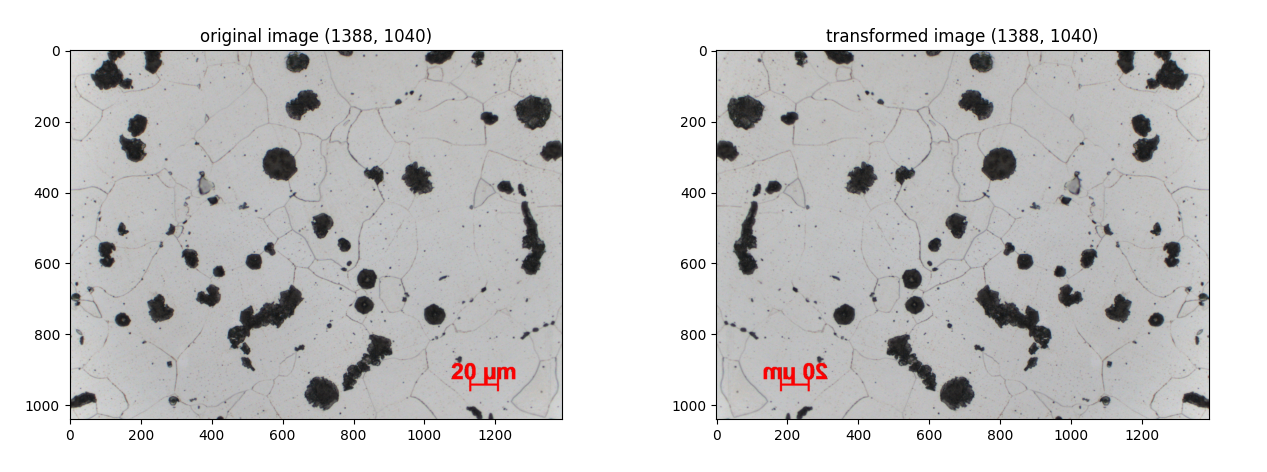
\includegraphics[width=1\textwidth]{rys.19.flipped.horizontally2.png}
    \caption{Wynik zastosowania techniki odbicia na przykładowym zdjęciu (po prawej). Widzimy, że rozmiary zdjęcia się nie zmieniają.  Żródło: opracowanie własne z~użyciem danych z~\cite{Pirowski17}}
    \label{fig:mesh19}
\end{figure}
Dzięki tej technice możliwe jest nawet czterokrotne powiększenie zestawu danych! Dodatkową, bardzo dużą zaletą tej metody jest fakt, że nie zmienia ona wymiarów obrazów. Jest to szczególnie korzystne, ponieważ posiadane  dane nie mają tej samej szerokości i~długości, co uniemożliwia wykorzystanie technik modyfikujących wymiary. Ze względu na dużą nierównowagę klas metoda ta jest wykorzystywana głównie do kompensowania liczności klas rzadkich. Przykład odbicia horyzontalnego został przedstawiony na rysunku \ref{fig:mesh19}.
















\chapter{Eksperymenty i~wyniki}
\label{cha5}

W tym rozdziale zostały przedstawione wszystkie wykonane badania wraz z~ich wynikami. W~badaniach zostały uwzględnione wszystkie metody uczenia maszynowego przedstawione w~rozdziale \ref{cha:ucz.masz} rozszerzając podejścia przytoczone w~przeglądzie literatury (rozdział \ref{cha:stan.badan}). Badania te stanowią uzupełnienie i~rozszerzenie prac z~\cite{Reczek21}. 

\section{Opis podejścia}
\label{opis_podejścia}
%  (czym się różni od tego z~rozdz. 2)
Badania te zostały podzielone na dwa duże etapy. Pierwszy z~nich polegał na rozpoznawaniu pojedynczych struktur obecnych na zdjęciach mikrostruktur. Wiązało się to z~wyznaczeniem konturów tych obiektów, następnie ich wycięcie i~utworzenie z~nich bazy danych, co wymagało „ręcznego” przyporządkowania obrazów do siedmiu klas. Następnie, za pomocą tego zestawu danych możliwe byłoby wyuczenie sieci neuronowej rozpoznającej te kształty. Eksperymenty rozpoczęto od przetestowania momentów Hu oraz tekstur Haralicka w~celu sklasyfikowania całych zdjęć mikrostruktur i~stwierdzenia których kształtów jest najwięcej. Następnym krokiem było przetestowanie uogólnionej transformaty Hougha. Po zakończeniu tych testów rozpoczęto badania nad bardziej skomplikowanymi metodami, które można byłoby zastosować bardziej automatycznie. Szczegóły dotyczące wycinania, tworzenia bazy danych i~rozpoznawania tych struktur zostały przedstawione w~rozdziałach \ref{wycinanie.struktur} oraz \ref{klasyfikacja.struktur}, które to zostały w~całości poświęcone temu etapowi.

Drugi etap polegał na ocenie jakości odlewów za pomocą technik wypracowanych w~pierwszej fazie, wykorzystując klasyczne klasyfikatory, ale również posługując się sieciami neuronowymi. W~pierwszej kolejności wykorzystano momenty Hu w~celu wyłuskania z~obrazów cech, za pomocą których można byłoby przeprowadzić klasyfikację. Analogicznie przetestowano tekstury Haralicka. Cechy te podawano na wejście klasycznych klasyfikatorów, które zostały przedstawione w~rozdziale \ref{cha:Wykorzystane metody uczenia maszynowego}. Następnie przeprowadzono kompleksowe badania, w~których wykorzystywano liczbę struktur konkretnych klas znajdujących się na zdjęciach mikrostruktur, a~także klasyczne klasyfikatory. Wszystkie otrzymane wyniki porównano uwzględniając wiele aspektów, jak interpretowalność wyników, łatwość implementacji, prostotę algorytmu czy czas uczenia. Aby mieć ogląd całej sytuacji przetestowano również najskuteczniejsze obecnie architektury sieci neuronowych wykorzystywanych w~celach klasyfikacji obrazów i~również zostały one porównane wielopłaszczyznowo z~pozostałymi strategiami.

% ############ Klasyfikacja struktur #############
\section{Klasyfikacja struktur}
\label{sec:klasyfikacja_struktur}

Jest to najszerszy obszar badań, ponieważ dzięki danym w~postaci zliczonych struktur można sprawdzić, czy kształty tych struktur mają wpływ na właściwości mechaniczne odlewów, a~jeśli tak, to w~jakim stopniu. Jak dobrze wiadomo, sieci neuronowe, które otrzymują obrazy w~postaci pikseli jako dane wejściowe i~zwracają wynik w~postaci „tak” lub „nie” odpowiadając na pytanie, czy wytrzymałość na rozciąganie danej mikrostruktury jest duża (lub mała) są modelami „czarnej skrzynki”, co oznacza, że trudno zweryfikować, dlaczego model podjął jedną decyzję nad drugą. Wykorzystując jednak dane w~postaci liczby struktur i~ich klas, można pokusić się o~zbudowanie interpretowalnego modelu. W~tym celu zostanie przetestowany szereg metod, z~pomocą których będziemy w~stanie wyodrębnić poszczególne obiekty na zdjęciach mikrostruktur, a~następnie, za pomocą modelu sieci neuronowej będziemy mogli je rozpoznawać. 

% ############ Klasyfikacja struktur ###################
\subsection{Uogólniona transformata Hougha}
\label{hough}

Jako pierwsze podejście zostały przetestowane momenty Hu oraz tekstury Haralicka. Metody te zostały również wykorzystane do oceny wytrzymałości odlewów, których zasada działania była podobna, aczkolwiek była ona bardziej rozbudowana, stąd odsyłamy do rozdz. \ref{sec:hu_haralick}, gdzie została szczegółowo opisana. W~tym rozdziale zajmiemy się uogólnioną transformatą Hougha (ang. \ita{generalised Hough transform}, \bo{GHT}), która została przebadana jako następna. Stąd wykorzystano otwartoźródłową bibliotekę \ita{general-hough} \cite{generalhough}.
\begin{figure}[h]
    \centering
    
\includegraphics[width=0.5\textwidth]{rys.21.ght.duza.kulka.png}
    \caption{Wykrywanie kształtu przedstawionego na obrazie referencyjnym (ang. \ita{reference image}) w obrazie zapytania (ang. \ita{query image}). W~prawym dolnym rogu na czerwono zaznaczono wykryte kształty. Żółty krzyżyk oznacza punkt, który został wybrany za najbardziej podobny do referencyjnego, którym w~tym przypadku jest czarne koło. Żródło: opracowanie własne przy wykorzystaniu biblioteki \ita{general-hough}}
    \label{fig:mesh21}
\end{figure}
Ta strategia jest bardziej skoncentrowana na pojedynczych strukturach i~ich detekcji. Początkowe zmagania pokazały, że znajdowanie pojedynczych struktur danej klasy z~pomocą tej metody jest możliwe, aczkolwiek nie wszystkie kształty są wykrywane, a~niekiedy zdarzają się nawet większe pomyłki, co przedstawiono na powyższym rysunku (rys. \ref{fig:mesh21}). Natomiast na rysunkach \ref{fig:mesh22} i~\ref{fig:mesh23}) pokazano wyniki dla zmodyfikowanych danych wejściowych oraz obrazów referencyjnych. Chociaż uważa się, że GHT ma zalety takie jak:
\begin{itemize}
	\item odporność na częściowe lub nieznaczne zniekształcenie formy
	\item odporność na obecność innych struktur na obrazie,
	\item odporność na szum,
	\item możliwość znajdowania wielu wystąpień danego kształtu na obrazie wejściowym.
\end{itemize}
Pomimo tego, że metoda ta została stworzona właśnie do rozpoznawania form zdefiniowanych matematycznie (takie występują na naszych obrazach), jego działanie nie spełniło naszych oczekiwań.
\begin{figure}[h]
    \centering
    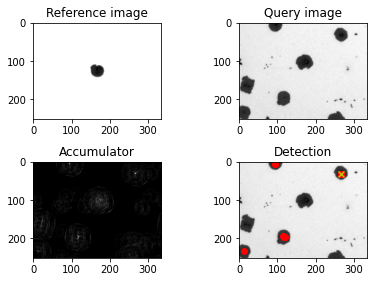
\includegraphics[width=0.6\textwidth]{rys.22.ght.mala.kulka.png}
    \caption{Działanie metody GHT na tym samym obrazie zapytania, lecz jako obraz referencyjny została użyta rzeczywista struktura znajdująca się na jednym ze zdjęć. Dodatkowo skala tej struktury jest taka sama, jak skala struktur na obrazie zapytania. Żródło: opracowanie własne przy wykorzystaniu biblioteki \ita{general-hough}}
    \label{fig:mesh22}
\end{figure}
Spoglądając na rys. \ref{fig:mesh21} można zauważyć dwa problemy. Po pierwsze, nie wykryto wszystkich kształtów. Po drugie, czerwone kropki oznaczające wykryty kształt niekiedy znajdują się na szarym tle, zamiast na czarnym kształcie. Ale to nie jedyne problemy. Zdarza się również, iż dana struktura jest oznaczona wielokrotnie. Dlatego zdecydowano się poeksperymentować z~obrazami referencyjnymi, co potencjalnie może poprawić wyniki. Na kolejnym rysunku \ref{fig:mesh22} możemy zauważyć, że obraz zapytania jest wciąż ten sam, natomiast zmienił się obraz referencyjny. Tym razem jest to rzeczywista struktura, a~więc nie jest ani idealnie czarna, ani idealnie okrągła. Dodatkowo jej skala jest taka sama, jak skala struktur na obrazie zapytania. Możemy również zaobserwować na obrazie z~wykrytymi kształtami (ang. \ita{detection}), iż tym razem czerwone kropki są rozmieszczone o~wiele bardziej precyzyjnie. 
\begin{figure}[h]
    \centering
    
\includegraphics[width=0.6\textwidth]{rys.23.ght.mala.kulka.bez.szarosci.png}
    \caption{Kolejny test z~tym samym obrazem zapytania, a~także z~tym samym obrazem referencyjnym, co na rys. \ref{fig:mesh22}. Widzimy, że metoda zadziałała jeszcze lepiej, gdyż wykryła poprawnie jeszcze jedną strukturę. Żródło: opracowanie własne przy wykorzystaniu biblioteki \ita{general-hough}}
    \label{fig:mesh23}
\end{figure}
Jednakże wciąż metoda ta nie jest na wystarczająco dokładna. W~kolejnych testach usunięto dodatkowo szare tło z~obrazów zapytania, przez co szare struktury znalazły się po tych przekształceniach na białym tle. Przykładowe wyniki zostały zaprezentowane na obrazie \ref{fig:mesh23}. Możemy zauważyć, że ten zabieg przyniósł oczekiwane efekty, a~mianowicie wykryto poprawnie o~jeden kształt więcej, niż przed tym zabiegiem.
Mimo wszystko takie podejście jest mało praktyczne, gdyż dla różnych obrazów należałoby dobierać obrazki referencyjne zgodnie ze skalą struktur na obrazach. Dodatkowo, pomimo tego, iż jest zaledwie sześć klas tych struktur, potrzebowalibymy znacznie więcej przykładów, aby pokryć przypadki, w~których struktura jest zniekształcona, bądź nakłada się z~inną strukturą. A~więc wiemy już, że ta metoda nie może zostać wykorzystana w~dalszych badaniach, a~zatem należy wrócić do poszukiwań tej odpowiedniej metody.

\subsection{Detekcja krawędzi filtrem Canny'ego}
\label{canny}

Kolejne techniki były bardziej skoncentrowane na wycinaniu poszczególnych struktur, a~następnie kategoryzowaniu każdej z~nich niezależnie w~kolejnych fazach. W~tym celu wykorzystano pakiet \ita{opencv-python} (nazywana dalej \ita{cv}). Jednak w~pierwszym kroku opracowano algorytm do przeprowadzania prostego zliczania struktur bez rozróżniania klasy kształtu. Krawędzie struktur wykrywano metodą Canny'ego \cite{Canny86}. Dodatkowo przetestowano różne techniki rozmywania obrazu (ang. \ita{blur}), czy inaczej – wygładzania, m.in. uśrednianie (w pythonie \ita{cv.blur}), rozmycie gaussowskie (ang. \ita{Gaussian blur}, w~pythonie \ita{cv.GaussianBlur}), rozmycie środkowe (ang. \ita{median blurring}, w~pythonie \ita{cv.medianBlur}) i~filtrowanie dwustronne (ang. \ita{bilateral filtering}, w~pythonie \ita{cv.bilateralFilter}). 
W zależności od rozmiaru zastosowanego jądra (ang. \ita{kernel}) otrzymujemy różne efekty przy rozmyciu. Rysunek \ref{fig:mesh24} przedstawia trzy zdjęcia, z~których jeden jest oryginalny (pierwszy od prawej), a~dwa pozostałe to efekt zastosowania wykrywania krawędzi. W~pierwszym od lewej zastosowano antyaliasing (rozmiar jądra 5x5), podczas gdy w~środkowym obrazie nie.
\begin{figure}[h]
	\centering
	\begin{subfigure}{0.29\textwidth}
	    \centering
	    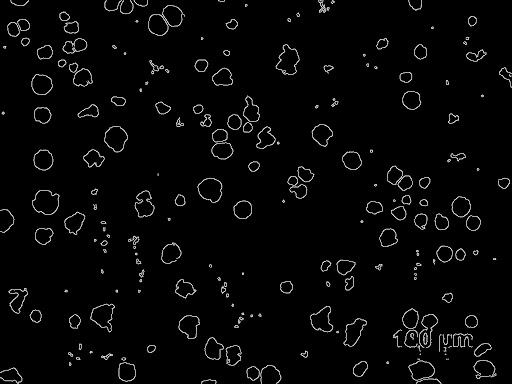
\includegraphics[width=1\textwidth]{rys.25a.canny.antialiasing.jpg} % pominalem obrazek 24, moze dodam kiedys
	    \subcaption{\label{subfigure_a}Wykrywanie krawędzi z~wykorzystaniem wygładzania}
	\end{subfigure}
	\begin{subfigure}{0.29\textwidth}
	    \centering
	    
\includegraphics[width=1\textwidth]{rys.25b.canny.jpg}
	    \subcaption{\label{subfigure_b}Wykrywanie krawędzi na oryginalnym obrazku}
	\end{subfigure}
	\begin{subfigure}{0.29\textwidth}
	    \centering
	    
\includegraphics[width=1\textwidth]{rys.25c.canny.original.jpg}
	    \subcaption{\label{subfigure_c}Oryginalne zdjęcie mikrostruktury}
	\end{subfigure}
	\caption{\label{fig:mesh24}Wykrywanie krawędzi z~wykorzystaniem filtra Canny'ego. Źródło: opracowanie własne}
\end{figure}
Wykryte struktury zostały następnie zliczone. Są to wszystie kontury widoczne na dwóch pierwszych obrazkach na rys. \ref{fig:mesh24}. Rysunek \ref{fig:mesh25} przedstawia przykład obrazu, dla którego algorytm wyliczył dziesięć takich struktur (czy też konturów).
\begin{figure}[h]
    \centering
    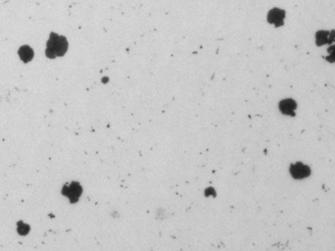
\includegraphics[width=0.35\textwidth]{rys.26.sample.image.strusctures.counting.png}
    \caption{Przykładowe zdjęcie mikrostruktury, dla którego wykryto 10 kształtów}
    \label{fig:mesh25}
\end{figure}
Zliczanie konturów przeprowadzono w~taki sposób, iż dla każdego obiektu obliczono pole powierzchni i~obwód. W~ten sposób można odrzucić kontury o~małej powierzchni lub małym obwodzie. Próg został dobrany empirycznie, tzn. dla testowanych progów wyświetlano wyniki wycinania kształtów i następnie wybrano próg, dla którego wyniki były najlepsze pod względem wizualnym (przede wszystkim ważne było, aby najmniejsze kształty, które ciężko sklasyfikować, zostały odrzucone). Wszystkie drobne, nieistotne kształty są eliminowane za pomocą tego podejścia. Podczas prób przebadano również takie metody jak progowanie (ang. \ita{threshold}), dylatacja (ang. \ita{dilation}), erozja (ang. \ita{erosion}) i~morfologia (ang. \ita{morphology}), co zostało przedstawione w rozdz. \ref{sec:normalizacja_skali}. Mimo wszystko najlepsze wyniki osiągnięto podczas zliczania struktur na oryginalnym zdjęciu.

\subsection{Wycinanie pojedynczych struktur z~obrazków}
\label{wycinanie.struktur}

Następnie, posiadając program (przygotowany samodzielnie), z~pomocą którego jesteśmy w~stanie wyznaczać kontury struktur, możemy spróbować je wycinać. Przyjęto strategię wycinania pojedynczych obiektów, a~następnie nakładania ich na białe tło. Struktury były umieszczane w~środku obrazu o~białym tle o~wymiarach 335 x 251 (szer. x wys.). Przykładowa wycięta struktura znajduje się na rys. \ref{fig:mesh26.pojedyncza}.
\begin{figure}[h]
    \centering
    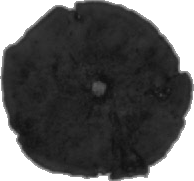
\includegraphics[width=0.25\textwidth]{rys.27.przykladowa.wycieta.struktura.png}
    \caption{Przykładowe zdjęcie wyciętej struktury (obraz przybliżony). Pozostałe kształty są wycinane analogicznie}
    \label{fig:mesh26.pojedyncza}
\end{figure}
Poniższe obrazki (rys. \ref{fig:mesh26} i~\ref{fig:mesh27}) przedstawiają działanie tego procesu. Tym samym kolorem zostały zaznaczone kształty, które zostały potraktowane jako jeden obiekt. Natomiast na rys. \ref{fig:mesh28} możemy zobaczyć przykładowe struktury, które zostały wycięte ze zdjęcia przedstawionego na rys. \ref{fig:mesh26}. 
\begin{figure}[h]
	\centering
	\begin{subfigure}{0.29\textwidth}
	    \centering
	    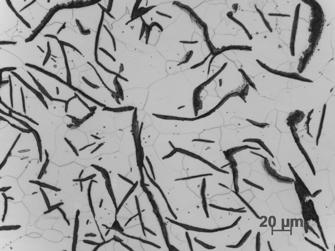
\includegraphics[width=1\textwidth]{rys.28a.wycinanie.struktur.png}
	    \subcaption{\label{subfigure_a}Zdjęcie mikrostruktury}
	\end{subfigure}
	\begin{subfigure}{0.29\textwidth}
	    \centering
	    
\includegraphics[width=1\textwidth]{rys.28b.wycinanie.struktur.png}
	    \subcaption{\label{subfigure_b}Wykryte struktury}
	\end{subfigure}
	\caption{\label{fig:mesh26}Działanie filtra Canny'ego. Każda wykryta struktura jest zaznaczona innym kolorem. Źródło: opracowanie własne}
\end{figure}
Struktury na obrazku oznaczone tym samym kolorem (a zatem uznane jako pojedynczy obiekt) są wycinane i~umieszczane na białym tle. Zostaną one wykorzystane do trenowania modeli kategoryzacji w~kolejnych fazach. Z~drugiej strony, jak widać na powyższym obrazie, wadą tej techniki jest to, że struktury są czasami ze sobą połączone, a~następnie traktowane przez algorytm jako jedna całość. Dzieje się tak najczęściej w~przypadku klas I~i~II (rys. \ref{fig:mesh14}), które są rozciągnięte na zdjęciach i~często się stykają ze sobą. 
\begin{figure}[h]
	\centering
	\begin{subfigure}{0.29\textwidth}
	    \centering
	    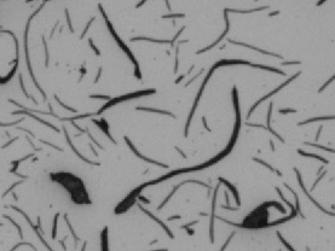
\includegraphics[width=1\textwidth]{rys.29a.wycinanie.struktur.png}
	    \subcaption{\label{subfigure_a}Zdjęcie mikrostruktury}
	\end{subfigure}
	\begin{subfigure}{0.29\textwidth}
	    \centering
	    
\includegraphics[width=1\textwidth]{rys.29b.wycinanie.struktur.png}
	    \subcaption{\label{subfigure_b}Wykryte struktury}
	\end{subfigure}
	\caption{\label{fig:mesh27}Kolejny przykład działania filtra Canny'ego. Każda wykryta struktura jest zaznaczona innym kolorem. Źródło: opracowanie własne}
\end{figure}
Próbowano tego uniknąć za pomocą takich algorytmów, jak erozja i~progowanie, ale te podejścia nie przyniosły zamierzonych rezultatów. Powyżej inny przykład działania tego samego algorytmu.
Algorytm na rys. \ref{fig:mesh27} zadziałał nieco lepiej niż na rys. \ref{fig:mesh26}. Jak widać, większość elementów została wycięta osobno. Tylko połączone kształty zostały wycięte jako jedna całość. Niestety nie ma na to uniwersalnego rozwiązania, ponieważ gdy ten problem zostanie rozwiązany, pojawia się nowy, jak np. brak wycinania mniej widocznych struktur lub wykrywanie wyblakłych struktur, które powinny zostać pominięte.
\begin{figure}[h]
	\centering
	\begin{subfigure}{0.29\textwidth}
	    \centering
	    
\includegraphics[width=1\textwidth]{rys.30a.wyciete.obiekty.png}
	\end{subfigure}
	\begin{subfigure}{0.29\textwidth}
	    \centering
	    
\includegraphics[width=1\textwidth]{rys.30b.wyciete.obiekty.png}
	\end{subfigure}
	\begin{subfigure}{0.29\textwidth}
	    \centering
	    
\includegraphics[width=1\textwidth]{rys.30c.wyciete.obiekty.png}
	\end{subfigure}
	\begin{subfigure}{0.29\textwidth}
	    \centering
	    
\includegraphics[width=1\textwidth]{rys.30d.wyciete.obiekty.png}
	\end{subfigure}
	\begin{subfigure}{0.29\textwidth}
	    \centering
	    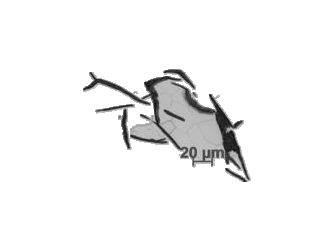
\includegraphics[width=1\textwidth]{rys.30e.wyciete.obiekty.png}
	\end{subfigure}
	\begin{subfigure}{0.29\textwidth}
	    \centering
	    
\includegraphics[width=1\textwidth]{rys.30f.wyciete.obiekty.png}
	\end{subfigure}
	\caption{\label{fig:mesh28}Przykładowe wycięte struktury z~rys. \ref{fig:mesh26}. Jak pokazały eksperymenty, zaliczenie tych kształtów do klasy I lub II nie miało większego wpływu na wynik klasyfikacji. Również stworzenie wspólnej klasy dla tych dwóch typów kształtów nie wpłynęło na wyniki. Źródło: opracowanie własne}
\end{figure}
Wycięte w~ten sposób obiekty (rys. \ref{fig:mesh28}) są wprowadzane na wejście sieci neuronowej (rozdział \ref{klasyfikacja.struktur}), która zostanie wytrenowana do kategoryzowania tych struktur. W~naszym zbiorze mamy siedem różnych klas. Sześć z~nich (rys. \ref{fig:mesh14}) to kształty wyróżnione w~normie \cite{norma}, natomiast autor dodał klasę siódmą, aby odróżnić te struktury od obiektów, które zostałe źle wycięte lub zawierających skalę, którą można znaleźć na wszystkich zdjęciach mikrostruktur. Wszystkie wycięte elementy były przechowywane lokalnie i~arbitralnie przypisywane do klas podczas tworzenia zbioru danych. Liczność tych klas jest następująca:
\begin{itemize}[label=\textbullet]
	\item klasa 0 – 14 przykładów (dodana przez autora),
	\item klasa I~– 278 przykładów,
	\item klasa II – 122 przykładów,
	\item klasa III – 292 przykładów,
	\item klasa IV – 76 przykładów,
	\item klasa V – 289 przykładów,
	\item klasa VI – 501 przykładów.
\end{itemize}
W następnym podrozdziale (tj. \ref{klasyfikacja.struktur}) zostały zaprezentowane badania związane z~klasyfikacją wyciętych struktur.

\subsection{Rozpoznawanie wyciętych struktur}
\label{klasyfikacja.struktur}

Na tym etapie badań posiadamy już własnoręcznie przygotowane dane dotyczące pojedynczych struktur obecnych na zdjęciach mikrostruktur (rys. \ref{fig:mesh14}). Ponownie, można by zacząć eksperymenty od takich najprostszych metod jak momenty Hu, momenty Zernike i~tekstury Haralicka wraz z~klasycznymi klasyfikatorymi, aczkolwiek takie podejście zostało już sprawdzone w~pracy \cite{Reczek21} i~pokazano, iż w~przypadku takich zestawów algorytmów oraz dostępnych danych, wyniki są porównywalne do tych, które otrzymujemy w~przypadku wykorzystania klasyfikatorów klasycznych z~weśjciem w~postaci pikseli. Dlatego tutaj przejdziemy od razu do bardziej zaawansowanych metod. W~tym celu zdecydowano się wykorzystać sieci neuronowe (rozdz. \ref{cha:Siecineuronowe}). W~szczególności zastosowano uczenie transferowe (rozdz. \ref{cha:cha3.5}) wykorzystując dobrze znaną sieć VGG19. 
\begin{figure}[h]
    \centering
    
\includegraphics[width=0.75\textwidth]{rys.31.confusion.matrix.better.quality.png}  %rys.31.confusion.matrix.png}
    \caption{Tablica pomyłek dla klasyfikacji struktur znajdujących się na zdjęciach mikrostruktur dla danych testowych. Żródło: opracowanie własne (z użyciem biblioteki \ita{seaborn})}
    \label{fig:mesh29}
\end{figure}
Implementacja tej architektury została uzyskana z~biblioteki \ita{Keras}. Podczas szkolenia sieć ta była wyłączona z~treningu. Dodatkowo, jej końcówka (tj. ostatnie kilka warstw odpowiadających za klasyfikację) nie została uwzględniona, natomiast dodano kilka dodatkowych warstw, które pozwoliły nam na douczenie sieci pod nasze dane. Zastosowano optymizator \ita{Adam}, wielkość paczki uczącej (ang. \ita{batch size}) wyniosła jeden, natomiast liczba epok wyniosła 100 (rys. \ref{fig:mesh30}). Pozostałe parametry zostały dostrojone. Taka sieć średnio osiąga wydajność około $82\%$ dla danych testowych (w przypadku danych treningowych dokładność waha się od $86\%$ do $95\%$ wydajności, w~zależności od konfiguracji), wartość metryki F1 wynosi $0.79$, natomiast wartość straty logistycznej (ang. \ita{logistic loss}) wyniosła $0.66$. Są to lepsze wyniki niż w~przytoczonej wcześniej pracy \cite{Reczek21} ze względu na to, że pracujemy na poprawionych danych, co zostało szczegółowo opisane w~przytoczonej pracy \cite{Reczek21}. Rysunek \ref{fig:mesh29} przedstawia tablicę pomyłek znormalizowaną względem wierszy (tj. rzeczywistych wartości). 
Po przeliczeniu na błąd względny otrzymujemy błędy na poziomie 10\%, 52\%, 26\%, 50\%, 49\% oraz 1\% odpowiednio dla klas od I~do VI (brak klasy „0” w~danych testowych ze względu na ich niską liczność). Błędy wynikają jednak głównie z~podobieństwa tych form w~ramach „sąsiadujących” klas takich jak klasy V i~VI (na rysunku są to klasy 4 i~5), gdzie prawie połowa kształtów z~klasy V jest sklasyfikowana jako klasa VI. Podobieństwo klas można dostrzec również na rys. \ref{fig:mesh14}, aczkolwiek jest to bardziej widoczne w~przypadku rzeczywistych danych, ponieważ większość tych kształtów zawiera cechy wielu klas (trudno im przypisać jedną konkretną cechę). Co więcej, baza danych została zbudowana arbitralnie przez autora, który nie jest ekspertem w~dziedzinie metalurgii. Rozbieżności w~dokładności predykcji między klasami są najprawdopodobniej związane z~brakiem zbalansowania w~ilości danych dostępnych dla każdej klasy.
\begin{figure}[h]
    \centering
    
\includegraphics[width=0.55\textwidth]{rys.32.vgg19.history.lepsza.jakosc.png}
    \caption{Historia dokładności modelu sieci neuronowej w~trakcie uczenia się. Są to rezultaty dla danych treningowych, gdzie najlepsze wyniki sięgają 87\%. Żródło: opracowanie własne (z wykorzystaniem biblioteki \ita{seaborn})}
    \label{fig:mesh30}
\end{figure}
Z drugiej strony wyniki wydają się być znacznie lepsze przy wykorzystaniu danych treningowych do ewaluacji. Po przeliczeniu błędów względnych otrzymujemy następujące wyniki: 36\% (klasa “0”), 0.4\%, 20\%, 7\%, 19\%, 38\% oraz 3\%. Możemy zaobserwować, że dane uczące mają znacznie mniej błędów względnych, co wskazuje, że wyniki można jeszcze poprawić. Dobrym kierunkiem może być zbalansowanie danych, gdyż, jak można zauważyć, najlepsze wyniki otrzymujemy dla klas, których liczba instancji była największa w~zbiorze (z wyjątkiem klasy V, aczkolwiek przykłady tej klasy są łudząco podobne do przykładów z~klasy VI). Przyjęto więc strategię, aby rozszerzyć dane z~tych klas, które jednocześnie mają najniższą skuteczność i~najmniej przykładów. Stąd zostaną rozszerzone klasy: „0", II, IV oraz V. Ponownie zostanie zastosowana (podobnie jak w~\ref{sec:hu_haralick}) metoda odbicia, która nie zmienia rozmiarów zdjęcia. Również tym razem zostanie zastosowana metoda odbicia horyzontalnego. Oprócz tego przetestowano jeszcze kilka innych podejść, jak nałożenie szumu na rozszerzone przykłady danych, a~także usunięcie szarości z~obrazów. Wyniki zostały przedstawione w~tab. \ref{structures.classification.different.approaches}. 
\begin{table}[h]
	\centering
	\begin{threeparttable}
		\caption{Podsumowanie różnych podejść co do klasyfikacji kształtów. Źródło: opracowanie własne}
		\label{structures.classification.different.approaches}
		\begin{tabularx}{1\textwidth}{ |X|X|X|X| }
		  \hline
		   \textbf{Augmentacja} & \textbf{Zaszumienie} & \textbf{Usuwanie szarości} & \textbf{Dokładność}\\

		  \hline
		  Nie & Nie & Nie & \bo{82.2\%}\\

		  \hline
		  Tak & Nie & Nie & 78\%\\

		  \hline
		  Tak & Tak & Nie & 79.7\%\\

		  \hline
		  Tak & Tak & Tak & 77.1\%\\
  		  
		  \hline
		  Tak (dod. klasę III) & Tak & Tak & 74.9\%\\
  		  
		  \hline
		\end{tabularx}
	\end{threeparttable}
\end{table}
A więc, jak możemy zauważyć, manipulacja danymi nie wpłynęła pozytywnie na wynik klasyfikacji. W~związku z~tym dalsze badania zostaną przeprowadzone na architekturze, dla której osiągnięto najlepsze wyniki. Biorąc pod uwagę niezbalansowanie klas oraz to, iż te dane były przygotowywane ręcznie przez autora tej pracy (który nie jest specjalistą w~dziedzinie metalurgii), w~celu poprawy wyników tej klasyfikacji najprawdopodobniej konieczne jest, aby przygotował je ekspert w~tej dziedzinie. Można to zadanie potraktować jako dalszą część prac, które byłyby rozszerzeniem niniejszej pracy. W~dalszych badaniach zostanie wykorzystana architekturu wraz z~danymi, dla których otrzymano najwyższe wyniki, tj. sieć neuronowa VGG19 wraz z~pierwotnie przygotowanymi obrazami struktur.
\begin{figure}[h]
    \centering
    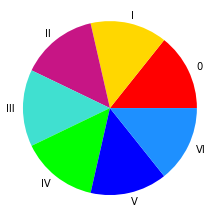
\includegraphics[width=0.50\textwidth]{rys.33.diagram.kolowy.legenda.png} % 52
    \caption{Legenda użytych kolorów w~celu oznaczenia struktur na obrazach, które należą do różnych klas. Żródło: opracowanie własne (z wykorzystaniem biblioteki \ita{matplotlib})}
    \label{rys.33.diagram.kolowy.legenda.png}
\end{figure}
Na rys \ref{rys.33.diagram.kolowy.legenda.png} została przedstawiona legenda. Każdy z~siedmiu kolorów przedstawionych na wykresie kołowym odpowiada jednej z~siedmiu klas strukur (zgodnie z~opisem na diagramie). Kolory te zostały dobrane za pomocą generatora wizualnie odmiennych kolorów, aby były jak najbardziej wyraziste. Poniżej przedstawiono przykłady klasyfikacji struktur z~wykorzystaniem opisanych powyżej metod. Na tych obrazach (rys. \ref{rys.34} - \ref{rys.38}) 
\begin{figure}[h]
	\centering
	\begin{subfigure}{0.42\textwidth}
	    \centering
	    
\includegraphics[width=1\textwidth]{rys.34a.pokolorowane.struktury.png}
	    \subcaption{\label{subfigure_a}Wykryte, sklasyfikowane i~ubarwione struktury}
	\end{subfigure}
	\begin{subfigure}{0.42\textwidth}
	    \centering
	    
\includegraphics[width=1\textwidth]{rys.34b.oryginalne.zdjecie.png}
	    \subcaption{\label{subfigure_b}Zdjęcie mikrostruktury}
	\end{subfigure}
	\caption{\label{rys.34}Zdjęcia mikrostruktury zawierające struktury klas I-III. Źródło: opracowanie własne}
\end{figure}
obowiązuje schemat, iż po prawej stronie znajduje się oryginalne zdjęcie mikrostruktury, natomiast po lewej stronie znajduje się to samo zdjęcie, z~tym że obecne tam struktury zostały pokolorowane zgodnie z~legendą (rys.~\ref{rys.33.diagram.kolowy.legenda.png}). Są to przykładowe zdjęcia, które 
\begin{figure}[h]
	\centering
	\begin{subfigure}{0.42\textwidth}
	    \centering
	    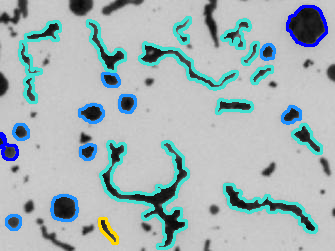
\includegraphics[width=1\textwidth]{rys.35a.pokolorowane.struktury.png}
	    \subcaption{\label{subfigure_a}Wykryte, sklasyfikowane i~ubarwione struktury}
	\end{subfigure}
	\begin{subfigure}{0.42\textwidth}
	    \centering
	    
\includegraphics[width=1\textwidth]{rys.35b.oryginalne.zdjecie.png}
	    \subcaption{\label{subfigure_b}Zdjęcie mikrostruktury}
	\end{subfigure}
	\caption{\label{rys.35}Zdjęcia mikrostruktury wraz ze strukturami klasy III, V i~VI. Można zauważyć również, że jedna, podłużna struktura została sklasyfikowana jako typ I. Źródło: opracowanie własne}
\end{figure}
dobrze reprezentują cały proces, który wygląda w~ten sposób, że dla każdego zdjęcia wejściowego przeprowadzane są operacje opisane w~rozdziale \ref{wycinanie.struktur}, a~następnie są one klasyfikowane przez architekturę przedstawioną
\begin{figure}[h]
	\centering
	\begin{subfigure}{0.41\textwidth}
	    \centering
	    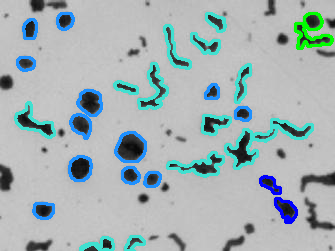
\includegraphics[width=1\textwidth]{rys.36a.pokolorowane.struktury.png}
	    \subcaption{\label{subfigure_a}Wykryte, sklasyfikowane i~ubarwione struktury}
	\end{subfigure}
	\begin{subfigure}{0.41\textwidth}
	    \centering
	    
\includegraphics[width=1\textwidth]{rys.36b.oryginalne.zdjecie.png}
	    \subcaption{\label{subfigure_b}Zdjęcie mikrostruktury}
	\end{subfigure}
	\caption{\label{rys.36}Zdjęcia mikrostruktury z~oznaczonymi formami grafitowymi, które należą do klas III-VI. Źródło: opracowanie własne}
\end{figure}
w~tym rozdziale. W~związku z~tym mogą wystąpić błędy, jak brak wykrycia danej struktury bądź źle sklasyfikowanie struktury.
\begin{figure}[h]
	\centering
	\begin{subfigure}{0.41\textwidth}
	    \centering
	    
\includegraphics[width=1\textwidth]{rys.37a.pokolorowane.struktury.png}
	    \subcaption{\label{subfigure_a}Wykryte, sklasyfikowane i~ubarwione struktury}
	\end{subfigure}
	\begin{subfigure}{0.41\textwidth}
	    \centering
	    
\includegraphics[width=1\textwidth]{rys.37b.oryginalne.zdjecie.png}
	    \subcaption{\label{subfigure_b}Zdjęcie mikrostruktury}
	\end{subfigure}
	\caption{\label{rys.37}Zdjęcia mikrostruktury zawierające kształty sklasyfikowane do klas IV oraz VI. Źródło: opracowanie własne}
\end{figure}
\begin{figure}[!h]
	\centering
	\begin{subfigure}{0.41\textwidth}
	    \centering
	    
\includegraphics[width=1\textwidth]{rys.38a.pokolorowane.struktury.png}
	    \subcaption{\label{subfigure_a}Wykryte, sklasyfikowane i~ubarwione struktury}
	\end{subfigure}
	\begin{subfigure}{0.41\textwidth}
	    \centering
	    
\includegraphics[width=1\textwidth]{rys.38b.oryginalne.zdjecie.png}
	    \subcaption{\label{subfigure_b}Zdjęcie mikrostruktury}
	\end{subfigure}
	\caption{\label{rys.38}Zdjęcia mikrostruktur przedstawiające kształty sklasyfikowane do klas III-VI. Źródło: opracowanie własne}
\end{figure}
%\clearpage
%\noindent 
%\afterpage{\clearpage}
Jak widzimy na przedstawionych rysunkach (rys. \ref{rys.34} – \ref{rys.38}), sieć klasyfikująca kształty wraz z~całą sekwencją rozpoznawania pojedynczych struktur przynosi całkiem przyzwoite efekty. Wizualnie nie można tutaj niczego skrytykować. Natomiast często zdarza się tak, jak już wspomniano wcześniej, że struktury te są bardzo podobne do siebie i~przygotowanie ich przez specjalistę w~dziedzinie metalurgii mogłoby przynieść znaczny wzrost skuteczności modelu.

Ostatnią próbą w~celu poprawienia skuteczności modelu było wyeliminowanie najmniejszych struktur z~klasyfikacji. Są one najbardziej problematyczne, gdyż wizualnie, praktycznie się nie różnią. Dodatkowo sam autor miał problem z~przypisaniem tych struktur do konkretnej klasy. Po usunięciu tych struktur otrzymaliśmy skuteczność na poziomie $82\%$, natomiast wartość straty logistycznej wynosi $0.8$, co jest bardzo dobrym wynikiem. Tablica pomyłek została przedstawiona na rys. \ref{rys.39.confusion.matrix.big.structures.png}. 
\begin{figure}[h]
    \centering
    
\includegraphics[width=0.7\textwidth]{rys.39.confusion.matrix.big.structures.better.quality.png}  %rys.39.confusion.matrix.big.structures.png}
    \caption{Tablica pomyłek dla klasyfikacji struktur znajdujących się na zdjęciach mikrostruktur dla danych testowych. Wykorzystano większe struktury, które zostały wybrane na podstawie zajmowanej przez nie powierzchni, jak również ich obwodu. Żródło: opracowanie własne (z użyciem biblioteki \ita{seaborn})}
    \label{rys.39.confusion.matrix.big.structures.png}
\end{figure}
Porównując tę tablicę pomyłek do poprzedniej, która dotyczyła wyników badań przeprowadzonych na wszystkich danych możemy dojść do kilku ciekawych wniosków. Otóż jak pokazano w~rozdz. \ref{wycinanie.struktur}, liczba struktur klasy „0"~wynosi zaledwie 14 i~została dodana przez autora pracy. W~tym wypadku ta klasa jest najmniej interesująca. 
Największe straty zanotowały klasy II oraz V, bo 7 i~10 punktów procentowych (odpowiednio). Natomiast największe zyski zanotowały klasy IV oraz VI, bo aż 33 i~6 punktów procentowych.

\subsection{Wnioski}
\label{klasyfikacja.struktur.wnioski}

Po badaniach nad zagadnieniem przedstawionym w~tym rozdziale można wyciągnąć wiele interesujących wniosków:
\begin{itemize}
	\item w~pierwotnym zbiorze występowały zdjęcia (przykładowo rys. \ref{fig:mesh15}), które nie nadawały się do tej analizy, gdyż nie zawierały w~sobie głównych form grafitowych (rys. \ref{fig:mesh14}), aczkolwiek była to zdecydowana mniejszość,
	\item GHT zwracała dosyć precyzyjne wyniki (rys. \ref{fig:mesh23}), jednak miała wiele obostrzeń, przede wszystkim konieczność zastosowania identycznego obrazka referencyjnego do poszukiwanego, mimo to do innych zastosowań może być skutecznie wykorzystywana,
	\item gdy wykorzystano rozmycie gaussowskie (ang. \ita{Gaussian blur}), popękane struktury były wykrywane lepiej (gdyż pęknięcia nie były uznawane za struktury). Również klasy V-VI zyskiwały na skuteczności, natomiast traciły na tym pozostałe klasy (przede wszystkim I-II),
	\item przetestowano również progowanie obrazu (ang. \ita{thresholding}), które polega na binaryzowaniu zdjęć, tj. przypisywaniu im czarnych bądź białych pikseli w~zależności od poprzedniej wartości tych pikseli. Miało to zapobiegać traktowaniu pęknięć jako struktury, jednakże całkowita skuteczność również spadła.
\end{itemize}

\section{Ocena jakości odlewów}
\label{Ocena jakości odlewów}

Jest to drugi najszerszy obszar badań (obok rozdz. \ref{sec:klasyfikacja_struktur}), gdyż jest to główny punkt tych badań oraz temat niniejszej pracy. Zebrano i~przedstawiono tutaj wszystkie testy związane z~oceną jakości odlewów. Eksperymenty przedstawiono w~kolejności, w~jakiej zostały wykonywane, tj. od najprostszych metod do najbardziej skomplikowanych, które jednocześnie zwracały najlepsze wyniki. Badanie rozpoczęto od sprawdzenia skuteczności klasycznych klasyfikatorów na danych w~postaci momentów Hu oraz tekstur Haralicka (rozdz. \ref{sec:hu_haralick}). Następnie przetestowano klasyczne klasyfikatory, które jako dane wejściowe dostawały poprzednio przygotowane dane w~postaci liczności struktur poszczególnych klas. Jako ostatnie zbadano skuteczność sieci neuronowych oraz dodatkowo podejście hybrydowe, w~którym wynik klasyfikacji sieci VGG19 dołączono do wejścia klasycznych klasyfikatorów (a więc otrzymywały one liczność struktur oraz wynik klasyfikacji sieci VGG19). 

%%%%%%%%% HU i HARALICK %%%%%%%%%%%%
\subsection{Momenty Hu oraz tekstury Haralicka}
\label{sec:hu_haralick}

Pierwszym podejściem było wykorzystanie tekstur Haralicka i~momentów Hu do zidentyfikowania struktur na zdjęciu. Implementacja metody momentów Hu została zaczerpnięta z~pakietu \ita{opencv-python}, natomiast implementacja tekstur Haralicka została zaczerpnięta z~modułu \ita{mahotas}. Może się wydawać, że użycie tych algorytmów jest poprawne i~przyniesie pożądane rezultaty, ponieważ zostały zaprojektowane specjalnie do tego celu. Rysunek \ref{fig:mesh20} przedstawia dwa zdjęcia różnych mikrostruktur, które potencjalnie można zidentyfikować przy użyciu technik opisanych powyżej.
\begin{figure}[h]
	\centering
	\begin{subfigure}{0.47\textwidth}
	    \centering
	    
\includegraphics[width=1\textwidth]{rys.20.przyklad.mikrostruktur.a.png}
	    \subcaption{\label{subfigure_a}Zdjęcie mikrostruktury z~obiektami klasy I~(rys. \ref{fig:mesh14})}
	\end{subfigure}
	\begin{subfigure}{0.47\textwidth}
	    \centering
	    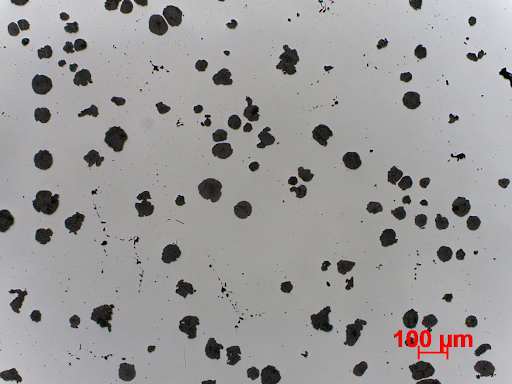
\includegraphics[width=1\textwidth]{rys.20.przyklad.mikrostruktur.b.png}
	    \subcaption{\label{subfigure_b}Zdjęcie mikrostruktury z~obiektami klasy V (rys. \ref{fig:mesh14})}
	\end{subfigure}
	\caption{\label{fig:mesh20}Dwa przykładowe zdjęcia mikrostruktur. Ich tekstury i~znajdujące się tam kształty diametralnie się różnią. Źródło: \cite{Pirowski17}}
\end{figure}
W pierwszym eksperymencie wykorzystano tekstury Haralicka, momenty Hu, a~także modele maszyny wektorów nośnych (SVM) oraz lasów losowych (RF, RFC). Testy zostały przeprowadzone na zbiorze danych klasyfikowanych ze względu na wytrzymałość na rozciąganie. Niestety taka konfiguracja modeli i~metod nie przyniosła oczekiwanych rezultatów. Testy przeprowadzono z~wykorzystaniem sprawdzianu krzyżowego (ang. \ita{cross-validation}), a~dokładnie sprawdzian \ita{k}-krotny (rozdz. \ref{cross.validation}), w~którym oryginalna próba jest dzielona na \ita{k} podzbiorów, po czym każdy z~tych podzbiorów jest wykorzystywany jako zbiór testowy, gdzie w~tym czasie wszystkie pozostałe są wykorzystywane jako zbiór treningowy.
\begin{table}[!h]
	\centering
	\begin{threeparttable}
		\caption{Wyniki klasyfikacji binarnej z~użyciem klasycznych klasyfikatorów, z~wykorzystaniem momentów Hu oraz tekstur Haralicka. Źródło: opracowanie własne}
		\label{hu_haralick_table}
		\begin{tabularx}{1\textwidth}{ |X|X|X|X| }
		  \hline
		  \textbf{Model} & \textbf{Typ wejścia} & \textbf{Wagi klas} & \textbf{Dokładność}\\

		  \hline
		  SVM & Hu\tnote{a} & — & 71.5\%\\

		  \hline
		  SVM & Haralick\tnote{b} & — & 71.5\%\\

		  \hline
		  SVM & Hu + Haralick\tnote{c} & — & 71.5\%\\

		  \hline
		  RFC & Hu & zrównoważone & 58\%\\

		  \hline
  		  RFC & Haralick & zrównoważone & 70\%\\
  		  
		  \hline
  		  RFC & Hu + Haralick & zrównoważone & 70.1\%\\
  		  
		  \hline
		\end{tabularx}
		\begin{tablenotes}
			\footnotesize
			\item[a] Momenty Hu wyliczone ze zdjęć (7 elementów).
			\item[b] Tekstury Haralicka wyznaczone ze zdjęć (13 elementów).
			\item[c] Konkatenacja wyników dwóch powyższych metod (20 elementów).
		\end{tablenotes}
	\end{threeparttable}
\end{table}
 Następnie te \ita{k} rezultatów jest uśrednianych. 
Wyniki zaprezentowano w~tabeli \ref{hu_haralick_table}.
\begin{table}[h]
	\centering
	\begin{threeparttable}
		\caption{Wyniki klasyfikacji binarnej z~użyciem klasycznych klasyfikatorów, z~wykorzystaniem momentów Hu oraz tekstur Haralicka. Dodatkowo rozszerzono dwukrotnie liczbę zdjęć o~niskiej odporności (augmentacja). Źródło: opracowanie własne}
		\label{hu_haralick_table_with_augmentation}
		\begin{tabularx}{1\textwidth}{ |X|X|X|X| }
		  \hline
		  \textbf{Model} & \textbf{Typ wejścia} & \textbf{Wagi klas} & \textbf{Dokładność}\\

		  \hline
		  SVM & Hu & — & 55.7\%\\

		  \hline
		  SVM & Haralick & — & 54.6\%\\

		  \hline
		  SVM & Hu + Haralick & — & 54.6\%\\

		  \hline
		  RFC & Hu & zrównoważone & 56.6\%\\

		  \hline
  		  RFC & Haralick & zrównoważone & 86\%\\
  		  
		  \hline
  		  RFC & Hu + Haralick & zrównoważone & 86\%\\
  		  
		  \hline
		\end{tabularx}
	\end{threeparttable}
\end{table}
Jak widzimy, wyniki dla większości tych metod wynoszą około 71\%. Nieco gorszy wynik w~przypadku lasu losowego może wynikać z~zastosowania zrównoważenia wag klas. Jednakże zbiór danych składa się z~3358 zdjęć o~wysokiej wytrzymałości na rozciąganie oraz 1337 zdjęć o~niskiej wytrzymałości na rozciąganie (patrz \ref{sec:normalizacja_przyblizenia}). A~więc liczba zdjęć o~wysokiej wytrzymałości stanowi dokładnie 71\% wszystkich danych, stąd klasyfikatory zamiast rzeczywiście rozpoznawać dane tak na prawdę mogą dopasowywać się do częstotliwości występowania zdjęć określonej klasy. Stąd przeprowadzono dodatkowe testy z~wykorzystaniem augmentacji (patrz \ref{cha:cha3.4}, \ref{sec:augmentacja}). Konkretnie zastosowano metodę odbicia na mniej licznej klasie (a więc na zdjęciach o~niskiej wytrzymałości), dzięki czemu stosunek liczby zdjęć o~wysokiej wytrzymałości do liczby wszystkich zdjęć spadł z~71\% do 55.7\%. Wyniki po przeprowadzeniu augmentacji znajdują się w~tab. \ref{hu_haralick_table_with_augmentation}.
\begin{table}[h]
	\centering
	\begin{threeparttable}
		\caption{Wyniki klasyfikacji binarnej z~użyciem klasycznych klasyfikatorów, z~wykorzystaniem momentów Hu oraz tekstur Haralicka. Dane dodatkowo zostały zaszumione, aby zapobiec nadmiernemu dopasowaniu się modelu do danych. Źródło: opracowanie własne}
		\label{hu_haralick_table_with_augmentation_and_noise}
		\begin{tabularx}{1\textwidth}{ |X|X|X|X| }
		  \hline
		  \textbf{Model} & \textbf{Typ wejścia} & \textbf{Wagi klas} & \textbf{Dokładność}\\

		  \hline
		  SVM & Hu & — & 55.7\%\\

		  \hline
		  SVM & Haralick & — & 55.5\%\\

		  \hline
		  SVM & Hu + Haralick & — & 55.5\%\\

		  \hline
		  RFC & Hu & zrównoważone & 51.6\%\\

		  \hline
  		  RFC & Haralick & zrównoważone & 72.2\%\\
  		  
		  \hline
  		  RFC & Hu + Haralick & zrównoważone & 72.6\%\\
  		  
		  \hline
		\end{tabularx}
	\end{threeparttable}
\end{table}
Dodatkowo, aby nie zwiększać sztucznie dokładności ze względu na podobieństwo danych wygenerowanych sztucznie i~oryginalnych, postanowiono nałożyć szum na dane wygenerowane syntetycznie. Zdecydowano się na szum biały. Wyniki zostały przedstawione w~tabeli \ref{hu_haralick_table_with_augmentation_and_noise}.

Porównując wyniki otrzymane w~tych trzech eksperymentach można dojść z~pewnością do kilku wniosków. Po pierwsze, widać wyraźnie, że wyniki pomiędzy modelami drzew oraz maszyny wektorów znacząco się różnią. W~pierwszym eksperymencie wyniki dla SVM są lepsze od 1 do nawet 12 punktów procentowych. W~pozostałych dwóch eksperymentach wyniki dla SVM są znacznie gorsze od tych dla lasu losowego, w~ekstremalnym przypadku aż o~30 punktów procentowych. Po drugie, można zauważyć, że w~większości przypadków wyniki dla momentów Hu są najgorsze, co można wytłumaczyć tym, iż jest to najprostsza metoda. Natomiast widzimy również wpływ augmentacji danych, jak również zaszumienia danych. Można przyjąć, iż najbardziej wiarygodne wyniki otrzymaliśmy w~trzecim eksperymencie, gdyż, przede wszystkim, skuteczność algorytmu nie pokrywa się ze stosunkiem liczebności klas, oraz wyniki nie różnią się między sobą w~niewytłumaczalny sposób. Mimo wszystko, ciężko do końca ocenić co tak naprawdę wpłynęło na te wyniki. Dodatkowo to podejście ma bardzo niską interpretowalność, tzn. ciężko ocenić dlaczego model wybrał jedną decyzję, zamiast innej. Natomiast atutem tego podejścia jest czas wykonywania (czas uczenia modeli). Mimo ustawienia parametrów SVM na wiele iteracji, a~także ustawienie stosunkowo dużej liczby drzew dla algorytmu lasu losowego, czas uczenia tych modeli jest rzędu kilkunastu sekund. Jak widzimy, już nawet najprostsze metody dają pewne pozytywne rezultaty, dlatego zdecydowano się na nieco bardziej złożoną strategię, która być może podniesie skuteczność.

\subsection{Klasyfikacja za pomocą liczby struktur}
\label{Klasyfikacja za pomocą liczby struktur} % cha6

W następnym kroku przetestowano skuteczność klasycznych klasyfikatorów w~ocenie jakości odlewów (tj. predykcji wytrzymałości na rozciąganie odlewów). Jako dane wejściowe zastosowano liczbę struktur poszczególnych klas (rys. \ref{fig:mesh14}), które są pozyskiwane w~procesie przedstawionym w~rozdz. \ref{sec:klasyfikacja_struktur}. Stąd na wejście klasycznych klasyfikatorów jest podawana tablica siedmiu liczb, z~czego każda z~tych liczb odpowiada liczebności odpowiedniej klasy (tj. liczba „zerowa"~odpowiada liczebności obiektów klasy „0"~itd.) i~na podstawie tych danych starają się przewidzieć wytrzymałość na rozciąganie odlewów przedstawianych na zdjęciach, których te dane dotyczą. 
\begin{figure}[h]
    \centering
    \includegraphics[width=0.75\textwidth]{rys.41.flowchart.diagram.png}
    \caption{Schemat blokowy przedstawiający działanie klasyfikacji wytrzymałości na rozciąganie na podstawie liczności struktur poszczególnych klas. Żródło: opracowanie własne (z wykorzystaniem \href{https://www.lucidchart.com}{lucidchart})}
    \label{rys.41.flowchart.diagram.png}
\end{figure}
Przetestowano również podejścia, w~których zamiast bezwzględnych liczb podawano na wejście procentowy udział struktur poszczególnych klas, a~także strategie, w~której na wejście podawano wynik funkcji softmax (wzór \ref{eq.softmax}) na bezwzględnych licznościach struktur poszczególnych klas. Na rys. \ref{rys.41.flowchart.diagram.png} przedstawiono schemat działania całego procesu.
W~tym celu wykorzystano najpopularniejsze klasyfikatory, jak maszyna wektorów nonych (SVM), drzewo decyzyjne (DT), las losowy (RFC), regresja logistyczna (logit), perceptron wielowarstwowy (MLP) oraz AdaBoost. W~następnych podrozdziałach są przedstawione analizy oraz wyniki uzyskane z~użyciem wyżej wymienionych klasyfikatorów.

%%%%%%%%%%%%%%% SVM %%%%%%%%%%%%%%%%
\subsubsection{Klasyfikator SVM}
\label{structures.with.svm}

Jako pierwsze zostanie omówione podejście, w~którym jako klasycznego klasyfikatora użyto SVM, czyli maszynę wektorów nośnych (rozdz. \ref{cha:Maszyna wektorów nośnych}). Schemat ogólny został przedsawiony na rys. \ref{rys.41.flowchart.diagram.png}. W~pierwszej kolejności przebadano strategię, w~której na wejście SVM podawano bezwzględną liczbę struktur poszczególnych klas. Badania przeprowadzono wykorzystując walidację krzyżową (rozdz. \ref{cross.validation}) oraz przeszukiwanie siatki (rozdz. \ref{Optymalizacja hiperparametrów}). Użyto już gotowej implementacji z~biblioteki \ita{scikit-learn} pod nazwą \ita{GridSearchCV}, który obsługuje te dwie rzeczy naraz. W~rezultacie otrzymano model, który osiągnął $83.3\%$ dokładności dla danych testowych oraz około cztery punkty procentowe więcej dla danych treningowych ($86.7\%$). Wartość straty logistycznej wyniosła $0.39$. To oznacza, że nie doszło do przetrenowania, ani niedotrenowania modelu do danych, czemu też zapobiega sprawdzian krzyżowy. W~każdym razie wyniki wydają się być wysokie, tym bardziej, że opierają się na modelu, który miał mniejszą skuteczność (o pół punktu procentowego). Poniżej przedstawiono wykres krzywej Precision-Recall, który wskazuje jaka jest precyzja modelu (ang. \ita{precision}) przy zadanej czułości (ang. \ita{recall}). 
\begin{figure}[h]
    \centering
    \includegraphics[width=0.62\textwidth]{rys.42.krzywa.precision.recall.png}
    \caption{Wykres krzywej Precision-Recall. Średnia wartość precyzji wynosi 0.88. Żródło: opracowanie własne (z wykorzystaniem biblioteki \ita{scikit-learn})}
    \label{rys.42.krzywa.precision.recall.png}
\end{figure}
Natomiast na rys. \ref{rys.43.confusion.matrix.svm.unbalanced} przedstawiono tablicę pomyłek dla tej klasyfikacji.
\begin{figure}[h]
    \centering
    \includegraphics[width=0.45\textwidth]{rys.43.confusion.matrix.svm.unbalanced}
    \caption{Tablica pomyłek dla klasyfikacji wytrzymałości na rozciąganie odlewów. Użyto niezbalansowanych danych (oryginalny zbiór). Żródło: opracowanie własne (z wykorzystaniem biblioteki \ita{seaborn})}
    \label{rys.43.confusion.matrix.svm.unbalanced}
\end{figure}

Kolejnym przetestowanym pomysłem była strategia, w~której zamiast bezwzględnych liczb okrelających liczność struktur odpowiednich klas na wejście podawano procentowy udział struktur poszczególnych klas. Tym razem skuteczność wyniosła $78.7\%$, a~więc dokładnie o~cztery punkty procentowe mniej, niż w~przypadku liczności struktur. Średnia wartość precyzji wyniosła $0.8$, a~więc również gorzej niż w~poprzednim wypadku. Również wartość straty logistycznej jest większa i~wynosi $0.47$. Stąd wykres nie jest nawet wymagany, ponieważ po samych wynikach liczbowych możemy z~całą pewnością stwierdzić, iż tutaj lepiej zadziałało poprzednie podejście. Próbując wyjaśnić takie rozbieżności tak naprawdę ciężko dojść do sensownego wyjaśnienia tej sytuacji. Wydawać mogłoby się, iż wyniki powinny być znacznie bardziej zbliżone, a~to ze względu na charakter danych wejściowych. Procentowy udział struktur poszczególnych to nic innego jak znormalizowane wyniki biorące pod uwagę liczność struktur danej klasy względem wszystkich pozostałych. A~jednak wyniki są dużo gorsze. Natomiast wystąpiła jedna drobna różnica, a~mianowicie było dziewięć zdjęć, dla których nie wykryto ani jednej struktury, stąd niemożliwe było wyliczenie względnego udziału struktur poszczególnych klas, wskutek czego konieczne było ich wyeliminowanie ze zbioru. Tak czy inaczej, jest to tylko dziewięć przykładów spośród 4695 wszystkich, stąd można ten fakt pominąć. 

Jako ostatnia została przetestowana strategia, w~której na wejście klasycznych klasyfikatorów jest podawany wynik funkcji softmax na pierwotnych danych (tj. liczności struktur poszczególnych klas). W~tym przypadku otrzymaliśmy dokładność na poziomie $79\%$, średnią wartość precyzji równą $0.72$ oraz wartość straty logistycznej równą $0.51$. Jak widzimy, z~wszystkich trzech zasosowanych tutaj strategii najlepiej sprawdza się bezwzględna liczność struktur poszczególnych klas, dlatego w~dalszych badaniach będziemy się głównie skupiać na tego typu danych. 

Jednakże dane są mocno niezbalansowane, co zostało pokazane w~rozdz. \ref{sec:normalizacja_przyblizenia}. W~ramach przypomnienia, zdjęć reprezentujących odlewy z~wysoką wytrzymałością na rozciąganie jest 3358, natomiast tych z~niską jest 1337. To mogłoby wyjaśniać przesunięcie w~stronę klasy odpowiadającej wysokiej wytrzymałości, co zostało przedstawione na rys. \ref{rys.43.confusion.matrix.svm.unbalanced} (tzw. błąd drugiego rodzaju). Co prawda zgodnie z~terminologią jest to zaledwie „delikatnie niezbalansowany zbiór", aczkolwiek warto sprawdzić czy to niezrównoważenie ma wpływ na wyniki.
\begin{figure}[h]
    \centering
    \includegraphics[width=0.45\textwidth]{rys.44.confusion.matrix.svm.balanced}
    \caption{Tablica pomyłek dla klasyfikacji wytrzymałości na rozciąganie odlewów. Dane zostały zbalansowane. Źródło: opracowanie własne (z wykorzystaniem biblioteki \ita{seaborn})}
    \label{rys.44.confusion.matrix.svm.balanced}
\end{figure}
W tym celu wykorzystano najprostszą technikę równoważenia zbiorów, a~mianowicie wyeliminowano z~danych nadmiarowe przykłady nadreprezentowanej klasy. W~ten sposób mamy teraz 1337 przykładów zarówno mikrostruktur wysokiej, jak i~niskiej wytrzymałości. Jednakże po zbalansowaniu klas problem nadal występuje (rys. \ref{rys.44.confusion.matrix.svm.balanced}). Przeprowadzono te same testy i~wartości wszystkich metryk się pogorszyły, mimo że tablica pomyłek po tym zabiegu wygląda nieco lepiej. Stąd wiadomo, że przesunięcie w~stronę klasy wysokich wytrzymałości nie jest kwestią niezbalansowania klas. Co jest przyczyną tego stanu rzeczy postaramy się dogłębniej wyjaśnić przy okazji testów kolejnych klasyfikatorów klasycznych, w~tym bardziej interpretowalnych (m.in. drzewa decyzyjne) w~kolejnych podrozdziałach.

Podsumowując wyniki badań dla SVM przygotowano szkic, w~którym są przedstawione zbiorczo zebrane wyniki (tab. \ref{svm.binary.summary.table}). 
\begin{table}[h]
	\centering
	\begin{threeparttable}
		\caption{Podsumowanie wyników klasyfikacji binarnej z~użyciem klasyfikatora SVM w~celu predykcji wytrzymałości na rozciąganie odlewów. Źródło: opracowanie własne}
		\label{svm.binary.summary.table}
		\begin{tabularx}{1\textwidth}{ |X|X|X|X| }
		  \hline
		  \textbf{Typ wejścia} & \textbf{Dokładność} & \textbf{AP\tnote{a}} & \textbf{Strata logistyczna}\\

		  \hline
		  Liczba struktur & \bo{82.7\%} & \bo{0.88} & \bo{0.39}\\

		  \hline
		  Procentowy udział struktur & 78.7\% & 0.8 & 0.47\\

		  \hline
		  Wartość funkcji softmax dla liczby struktur & 79\% & 0.72 & 0.51\\

		  \hline
		  Liczba struktur (zbalansowane dane)  & 78.4\% & 0.79 & 0.49\\
%
%		  \hline
%  		  Optuna i~kroswalidacja & \bo{84\%} & \bo{0.88} & \bo{5.66}\\
%  		  
		  \hline
		\end{tabularx}
		\begin{tablenotes}
			\footnotesize
			\item[a] AP – średnia wartość precyzji.
		\end{tablenotes}
	\end{threeparttable}
\end{table}
Widzimy, że najlepsze wyniki otrzymujemy dla oryginalnych danych wejściowych, tj. w~postaci liczności struktur poszczególnych klas, stąd w~kolejnych badaniach z~użyciem pozostałych klasyfikatorów skupimy się głównie na tego typu danych.
Dodatkowo, w~ramach próby uzyskania najlepszego możliwego wyniku skorzystano z~biblioteki \ita{Optuna}, która służy do optymalizacji hiperparametrów. Polega ona na nieco innym wyszukiwaniu, niż w~przypadku poprzedniego modułu. Po zastosowaniu kroswalidacji ta strategia przyniosła najlepsze wyniki. Dla danych w~postaci liczby struktur otrzymujemy $84\%$ dokładności, $0.88$ średniej wartości precyzji oraz $5.66$ wartości straty logistycznej.

%%%%%%%%% DRZEWO DECYZYJNE %%%%%%%%%%
\subsubsection{Drzewo decyzyjne}
\label{structures.with.dt}

W tym podrozdziale zajmiemy się wynikami osiąganymi za pomocą drzew decyzyjnych (\ref{cha:Drzewo decyzyjne}). Mimo, iż jest to bardzo prosty model, często zwraca przyzwoite wyniki, zaś jego interpretowalność jest jego największym atutem (obok jego prostoty). 
Jak wiemy istnieje wiele algorytmów generowania drzew decyzyjnych. Jako że autor czerpie implementacje klasycznych klasyfikatorów z~biblioteki \ita{scikit-learn}, toteż pierwszym przebadanym algorytmem będzie ten wykorzystywany przez wspomnianą bibliotekę. Jest to zoptymalizowana wersja algorytmu CART.
Ponownie rozpoczniemy od zaprezentowania wyników, gdy jako dane wejściowe wykorzystano bezwzględną liczność struktur poszczególnych klas. Testy podzielono względem głębokości testowanych drzew. Ponieważ wymiar danych wejściowych wynosi siedem, nie ma sensu bliżej przyglądać się drzewom o~głębokości większej niż trzy. Natomiast w~ramach porównania również one zostaną uwzględnione w~podsumowaniu. 
\begin{figure}[h]
    \centering
    \includegraphics[width=0.5\textwidth]{rys.45.decision.tree.depth.1}
    \caption{Wizualizacja drzewa decyzyjnego. Warunek jest przedstawiony w~pierwszym wierszu pierwszego klocka decyzyjnego. Sprawdzamy, czy struktur III typu jest mniej lub równo $2.5$. Na tej podstawie jest wyznaczana wytrzymałość odlewu. Źródło: opracowanie własne (z wykorzystaniem biblioteki \ita{graphviz})}
    \label{rys.45.decision.tree.depth.1}
\end{figure}
W pierwszej kolejności przeprowadzono badania dla drzew o~głębokości równej jeden. Dla takich drzew średnia dokładność modelu wynosi $78\%$, co już jest bardzo dobrym wynikiem. Wizualizacja takiego drzewa została przedstawiona na rys. \ref{rys.45.decision.tree.depth.1}. 
Jak możemy zauważyć, najważniejsze są tutaj struktury typu III (rys. \ref{fig:mesh14}). Biorąc pod uwagę tylko ten jeden typ struktur otrzymujemy dokładność na wspomnianym poziomie $78\%$. Zobaczmy teraz jak prezentują się wyniki dla drzewa o~głębokości równej dwa. Otóż dokładność wyniosła $81.2\%$, natomiast wizualizacja została przedstawiona na rys. \ref{rys.46.decision.tree.depth.2}. 
\begin{figure}[h]
    \centering
    \includegraphics[width=0.85\textwidth]{rys.46.decision.tree.depth.2}
    \caption{Wizualizacja drzewa decyzyjnego o~głębokości równej dwa. Źródło: opracowanie własne (z wykorzystaniem bibliteki \ita{graphviz})}
    \label{rys.46.decision.tree.depth.2}
\end{figure}
Jak możemy zauważyć, klasa III jest ponownie najważniejszą klasą, natomiast dochodzą nam również klasy I~oraz VI. Logicznym wytłumaczeniem tego stanu rzeczy może być fakt, iż właśnie struktury tych trzech klas najbardziej różnią się od pozostałych wizualnie. Dla drzewa o~głębokości równej trzy otrzymujemy dokładność na poziomie $81.3\%$, a~więc zaledwie jedną dziesiątą punktu procentowego więcej, niż dla drzewa o~głębokości dwa. To może świadczyć o~nadmiernym dopasowaniu się modelu do danych, czy też słabej generalizacji. Dla większych głębokości drzewa nie odnotowano wzrostu dokładności. Ciekawie również prezentują się wyniki dla innych typów wejść, toteż zostaną one przedstawione na samym końcu tej sekcji w~formie tabeli. 

Tymczasem przejdziemy do kolejnego algorytmu generowania drzewa decyzyjnego. Obok algorytmu CART przetestowano również algorytm ID3, którego implementacja została zaczerpnięta z~biblioteki \ita{decision-tree-id3}. 
\begin{figure}[h]
    \centering
    \includegraphics[width=0.55\textwidth]{rys.47.cart.vs.id3.czas.uczenia}
    \caption{Wykres przedstawiający czas uczenia modeli skonstruowanych przy pomocy różnych algorytmów generowania drzewa, w~zależności od jego głębokości. Źródło: opracowanie własne (z wykorzystaniem biblioteki \ita{matplotlib})}
    \label{rys.47.cart.vs.id3.czas.uczenia}
\end{figure}
Skonfrontowano ze sobą takie cechy, jak czas uczenia, czas zwracania wyników czy też dokładność. W~pierwszej kolejności przyjrzymy się czasom uczenia tych modeli w~zależności od wykorzystanego alogrytmu oraz głębokości drzew. Na rys. \ref{rys.47.cart.vs.id3.czas.uczenia} przedstawiono wyniki tego porównania.
Jak możemy zauważyć, czas uczenia jest wyraźnie dłuższy dla algorytmu ID3 i~rośnie wraz ze wzrostem głębokości drzewa. Jest to znana własność tych algorytmów, gdyż na ogół algorytm CART działa szybciej, szczególnie gdy korzystamy z~zoptymalizowanej wersji algorytmu CART. 

Następną metryką jest czas uzyskania wyniku. Wyniki tego porównania przedstawiono na rys. \ref{rys.48.cart.vs.id3.czas.wyniku}. 
\begin{figure}[h]
    \centering
    \includegraphics[width=0.5\textwidth]{rys.48.cart.vs.id3.czas.wyniku}
    \caption{Wykres przedstawiający czas uzyskania wyniku przez modele skonstruowane przy pomocy różnych algorytmów generowania drzewa, w~zależności od jego głębokości. Źródło: opracowanie własne (z wykorzystaniem biblioteki \ita{matplotlib})}
    \label{rys.48.cart.vs.id3.czas.wyniku}
\end{figure}
Jak możemy zauważyć na wykresie, również w~tym zestawieniu lepiej prezentuje się algorytm CART. Jego wyjście jest zwracane niemal natychmiast, natomiast na wyniki drzewa zbudowanego za pomocą algorytmu ID3 trzeba czekać dłużej i~czas ten wydłuża się jeszcze bardziej, gdy obsługujemy głębsze drzewa. 

Ostatnią metryką, która posłuży nam do porównania tych dwóch algorytmów będzie dokładność. 
\begin{figure}[h]
    \centering
    \includegraphics[width=0.5\textwidth]{rys.49.cart.vs.id3.dokladnosc}
    \caption{Wykres przedstawiający dokładność uzyskaną przez modele skonstruowane przy pomocy różnych algorytmów generowania drzewa, w~zależności od jego głębokości. Źródło: opracowanie własne (z wykorzystaniem biblioteki \ita{matplotlib})}
    \label{rys.49.cart.vs.id3.dokladnosc}
\end{figure}
Otóz postaramy się zbadać który algorytm generuje bardziej dokładne drzewa pod względem klasyfikacji. 
Jak wiadomo, różne algorytmy generowania drzewa stosują różne kryteria podziału drzewa. I~tak algorytm ID3 wykorzystuje entropię (ang. \ita{entropy}) lub też przyrost informacji (ang. \ita{information gain}). Z~drugiej strony algorytm CART może korzystać przykładowo z~miary nieczystości Giniego (ang. \ita{Gini impurity}). Stąd mogą wynikać rozbieżności w~dokładności tych drzew. Na rys. \ref{rys.49.cart.vs.id3.dokladnosc} przedstawiono porównanie tych wyników. 
Widzimy, że orientacyjnie wyniki są bardzo zbliżone. Nie można jednoznacznie stwierdzić które z~tych podejść jest dokładniejsze, gdyż w~zależności od głębokości raz jeden, raz drugi model osiąga nieznacznie lepsze wyniki. Jednakże biorąc pod uwagę poprzednie czynniki wydaje się, że algorytm CART może być faktycznie lepszym wyborem, głównie, jeśli trenujemy głębokie drzewo i~zależy nam na czasie, uwzględniając w~tym czas uzyskania wyników.

Na koniec, zanim przedstawimy tabelę podsumowująca wszystkie testy związane z~drzewem decyzyjnym, przyjrzymy się jeszcze wynikom osiąganym za pomocą drzewa decyzyjnego skonstruowanego przy pomocy algorytmu CART, gdy uprzednio zbalansujemy dane. 
Rys. \ref{rys.50.decision.tree.depth2.balanced} przedstawia wizualizację drzewa skonstruowanego za pomocą algorytmu CART używając optymalizacji hiperparametrów. Dokładność tego modelu wynosi $73.5\%$, a~więc zanotowaliśmy spadek o~$7.7$ punktu procentowego. 
\begin{figure}[h]
    \centering
    \includegraphics[width=0.85\textwidth]{rys.50.decision.tree.depth2.balanced}
    \caption{Wizualizacja drzewa decyzyjnego o~głębokości równej dwa. Dodatkowo zbalansowano dane oraz użyto optymalizacji hiperparametrów. Źródło: opracowanie własne (z wykorzystaniem biblioteki \ita{graphviz})}
    \label{rys.50.decision.tree.depth2.balanced}
\end{figure}
Możemy zauważyć, iż liczność struktury typu III jest tu decydująca. Gdy jest tych struktur pewna ilość (więcej niż dwie), to wtedy z~dużą pewnością możemy stwierdzić, iż struktura ma małą wytrzymałość na rozciąganie. W~przeciwnym przypadku (a więc gdy struktur jest mniej niż trzy) klasyfikacja nie jest już taka dokładna. Stąd można wyciągnąć wnioski, iż obecność struktur typu III powoduje, że struktura ma niską wytrzymałość na rozciąganie.
\begin{figure}[h]
    \centering
    \includegraphics[width=0.5\textwidth]{rys.51.confusion.matrix.dt.balanced}
    \caption{Tablica pomyłek dla klasyfikacji wytrzymałości na rozciąganie odlewów wykorzystując drzewo decyzyjne o~głębokości równej dwa. Testy przeprowadzono na zbalansowanych danych. Źródło: opracowanie własne (z wykorzystaniem biblioteki \ita{seaborn})}
    \label{rys.51.confusion.matrix.dt.balanced}
\end{figure}
Tablica pomyłek została przedstawiona na rys. \ref{rys.51.confusion.matrix.dt.balanced}. Jak można zauważyć, klasyfikacja jest nieco przesunięta w~stronę wysokiej wytrzymałości (klasa 1). Można to wytłumaczyć przy pomocy wizualizacji drzewa (rys. \ref{rys.50.decision.tree.depth2.balanced}). Gdy struktur typu III jest mniej niż trzy, dokładność naszej klasyfikacji wynosi około $69\%$ (lewe poddrzewo). A~ponieważ większość obecnych tam struktur ma wysoką wytrzymałość, stąd przesunięcie w~kierunku tej klasy. Natomiast widzimy również spadki skuteczności w~wykrywaniu wysokiej wytrzymałości, co nastąpiło wskutek ograniczenia liczby danych o~tej własności. O~ile wyniki są teraz bardziej wiarygodne, o~tyle widzimy, że za pomocą samych liczności struktur nie jestemy w~stanie stwierdzić z~bardzo wysoką skutecznością jaka jest wytrzymałość tej struktury. Stąd teza, iż sieci neuronowe oceniające tę cechę odlewów na podstawie pikseli mogą osiągać wyższe skuteczności wydaje się jeszcze bardziej prawdopodobna. 

Jako podsumowanie prac z~drzewami decyzyjnymi zostaje przedstawiony szkic (tab. \ref{dt.binary.summary.table}), który zawiera wyniki większości wartych uwagi testów, również tych, które nie zostały tutaj bliżej opisane.
\begin{table}[h]
	\centering
	\begin{threeparttable}
		\caption{Podsumowanie wyników klasyfikacji binarnej z~użyciem drzew decyzyjnych w~celu predykcji wytrzymałości na rozciąganie odlewów. Źródło: opracowanie własne}
		\label{dt.binary.summary.table}
		\begin{tabularx}{1\textwidth}{ |X|X|X|X|X| }
		  \hline
		  \textbf{Typ wejścia} & \textbf{Głębokość} & \textbf{Dane zbalansowane} & \textbf{Dokładność}\\

		  \hline
		  Liczność\tnote{a} & 1 & Nie  & 78\%\\

		  \hline
		   Liczność & 2 & Nie & 81.2\%\\

		  \hline
  		  Liczność & 2 & Tak & 73.5\%\\

		  \hline
		  Liczność & 3 & Nie & 81.4\%\\

		  \hline
		  Liczność & Brak limitu & Nie & \bo{84.3\%} \\

%		  \hline
%		\Xhline{3.1\arrayrulewidth}
%		\Xhline{1.5pt}
  		  \hline \hline
  		  Procent\tnote{b} & 1 & Nie & 75\%\\
  		  
		  \hline
  		  Procent & 2 & Nie & 79\%\\
  		  
		  \hline
  		  Procent & 3 & Nie   & \bo{80\%} \\

%		  \hline
%	          	\Xhline{3\arrayrulewidth}
%		\Xhline{1.5pt}
		  \hline \hline
  		  Softmax\tnote{c} & 1 & Nie   & 74.5\%\\

		  \hline
  		  Softmax & 2 & Nie   & 75\% \\

		  \hline
  		  Softmax & 3 & Nie   & \bo{78\%} \\

		  \hline
		\end{tabularx}
		\begin{tablenotes}
			\footnotesize
			\item[a] Liczność struktur poszczególnych klas.
			\item[b] Procentowy udział struktur poszczególnych klas.
			\item[c] Wartość funkcji softmax dla liczności struktur.
		\end{tablenotes}
	\end{threeparttable}
\end{table}
Oczywiście najlepsze wyniki otrzymujemy dla głębszych drzew. Jednakże warto zwrócić uwagę przede wszystkim na dwie rzeczy. Po pierwsze, po zbalansowaniu danych zanotowaliśmy znaczny spadek skuteczności, co już zostałe omówione wyżej w~tym podrozdziale. Po drugie, najwyższą dokładność uzyskujemy dla danych w~postaci bezwzględnej liczności struktur poszczególnych klas, nieco gorsze wyniki, gdy na wejściu podajemy procentowy udział struktur poszczególnych klas, a~najgorsze wyniki, gdy użyjemy funkcji softmax. Poniekąd jest zrozumiałe, że dla funkcji softmax otrzymujemy nieco gorsze wyniki, gdyż usuwa ona z~danych pewną informację. Natomiast spadek dla danych w~postaci procentowego udziału jest nietypowy, aczkolwiek podobne wyniki uzyskano dla modelu SVM. Proste wytłumaczenie może opierać się na tym, iż tak na prawdę większy wpływ na wytrzymałość struktur ma to, czy struktury konkretnej klasy w~ogóle wystąpiły niż stosunek ich liczności względem pozostałych klas.

%%%%%%%%%% LAS LOSOWY %%%%%%%%%
\subsubsection{Las losowy}
\label{structures.with.rfc}

Kolejny klasyfikator klasyczny, którego możliwości w~ocenie wytrzymałości na rozciąganie odlewów zostały przebadane, to las losowy (rozdz. \ref{cha:Las losowy}). 
\begin{figure}[!h]
    \centering
    \includegraphics[width=0.35\textwidth]{rys.52.confusion.matrix.rfc.unbalanced}
    \caption{Tablica pomyłek dla klasyfikacji wytrzymałości na rozciąganie odlewów wykorzystując las losowy. Testy przeprowadzono na danych niezbalansowanych. Źródło: opracowanie własne (z wykorzystaniem biblioteki \ita{seaborn})}
    \label{rys.52.confusion.matrix.rfc.unbalanced}
\end{figure}
Tutaj szczegółowo zostaną zaprezentowane wyniki uzyskane z~wykorzystaniem optymalizacji hiperparametrów oraz kroswalidacji, na danych oryginalnych oraz zbalansowanych. Natomiast w~tabeli na końcu podrozdziału zostaną przedstawione wszystkie znaczące wyniki, których testy były analogiczne do przedstawionych. 
W pierwszej kolejności przebadamy model dla danych oryginalnych (rozdz. \ref{sec:normalizacja_przyblizenia}). Otóż model ten uzyskał skuteczność na poziomie $83\%$, średnią wartość precyzji na poziomie $0.91$ oraz wartość funkcji straty logistycznej na poziomie $0.4$. Wartość metryki F1 wyniosła $0.89$. Ogólnie można stwierdzić, że wyniki są jak najbardziej poprawne, jednakże patrząc na wykres tablicy pomyłek (rys. \ref{rys.52.confusion.matrix.rfc.unbalanced}) ponownie widać to, co występowało w~poprzednich klasyfikatorach. Mianowicie jest to przesunięcie w~stronę klasy z~wysoką wytrzymałością. Dlatego powtórzymy te testy dla zbalansowanych danych i~porównamy je z~poprzednimi wynikami. 
Zbalansowane dane są tworzone na tej samej zasadzie, co w~rozdz. \ref{structures.with.svm}, tzn. wszystkie przykłady o~niskiej wytrzymałości są uwzględniane w~zbiorze (ponieważ jest ich zdecydowanie mniej), natomiast z~przykładów o~wysokiej wytrzymałości wybieramy losowo tyle przykładów, aby było ich tyle samo, co w~poprzedniej klasie. 
\begin{figure}[h]
    \centering
    \includegraphics[width=0.35\textwidth]{rys.53.confusion.matrix.rfc.balanced}
    \caption{Tablica pomyłek dla klasyfikacji wytrzymałości na rozciąganie odlewów dla algorytmu lasu losowego. Wykorzystano dane zbalansowane. Źródło: opracowanie własne (z wykorzystaniem biblioteki \ita{seaborn})}
    \label{rys.53.confusion.matrix.rfc.balanced}
\end{figure}
Wyniki, jakie udało się osiągnąć dla tego zestawienia, to dokładność na poziomie $80.9\%$, średnia wartość precyzji na poziomie $0.85$, wartość funkcji straty logistycznej na poziomie $0.47$ oraz wartość metryki F1 na poziomie $0.81$. Jak więc widzimy, zanotowano spadek tych metryk, jednakże nie jest on tak duży, jak w~przypadku drzew decyzyjnych (rozdz. \ref{structures.with.dt}). 
\begin{table}[!h]
	\centering
	\begin{threeparttable}
		\caption{Podsumowanie wyników klasyfikacji binarnej z~użyciem lasu losowego w~celu predykcji wytrzymałości na rozciąganie odlewów. Źródło: opracowanie własne}
		\label{rfc.binary.summary.table}
		\begin{tabularx}{1\textwidth}{ |X|X|X|X|X| }
		  \hline
		  \textbf{Typ wejścia} & \textbf{Dane zbalansowane} & \textbf{Dokładność}\\

		  \hline
		  Liczność\tnote{a} & Nie  & \bo{83\%} \\

		  \hline
		  Liczność & Tak & 80.9\%\\

		  \hline
  		  Procent\tnote{b} & Nie & 81.8\%\\

	          \hline
  		  Softmax\tnote{c} & Nie & 81.9\%\\

		  \hline
		\end{tabularx}
		\begin{tablenotes}
			\footnotesize
			\item[a] Liczność struktur poszczególnych klas.
			\item[b] Procentowy udział struktur poszczególnych klas.
			\item[c] Wartość funkcji softmax dla liczności struktur.
		\end{tablenotes}
	\end{threeparttable}
\end{table}
Na rys. \ref{rfc.binary.summary.table} przedstawiono tablicę pomyłek. Jak widzimy, zbalansowanie danych przyniosło oczekiwany efekt. Dodatkowo pokazało, że o~ile faktycznie zanotowano spadki w~skuteczności, o~tyle były one bardzo niewielkie, co dowodzi skuteczności tego podejścia. 
Tabela dodatkowo podsumowuje większość przeprowadzonych badań, które osiągnęły istotne wyniki.
Jak możemy zauważyć, tendencja skuteczności względem różnych typów wejścia jest zachowana. Ponownie najlepsze wyniki otrzymujemy na danych w~postaci liczności struktur, aczkolwiek wyniki pomiędzy różnymi typami wejścia nie różnią się znacząco. Ponadto wyniki dla danych zbalansowanych są zaledwie $2.1$ punktu procentowego gorsze od najlepszych wyników osiągniętych przy pomocy lasu losowego. 

%%%%%%%%%% REGRESJA LOGISTYCZNA %%%%%%%%%
\subsubsection{Regresja logistyczna}
\label{structures.with.logit}

Następnym modelem, który został przetestowany jest regresja logistyczna (rozdz. \ref{Regresja logistyczna}). Trzymając się schematu z~poprzednich podrozdziałów, ponownie przedstawimy szczegółowe wyniki dla danych w~postaci liczności klas dla danych niezbalansowanych i~zbalansowanych, po czym na końcu rozdziału zostanie przedstawiona tabela podsumowująca większość prac z~użyciem tego modelu. 
Jak się okazało, nieco nieoczekiwanie, wyniki dla regresji logistycznej były całkiem przyzwoite. Otóż zaczynając od danych niezbalansowanych, otrzymaliśmy następujące wyniki: $83.1\%$ dokładności, $0.91$ średniej wartości prezycji, $0.41$ wartości funkcji straty logistycznej oraz $0.88$ wartości metryki F1. Na rys. \ref{rys.54.confusion.matrix.logit.unbalanced} 
\begin{figure}[!h]
    \centering
    \includegraphics[width=0.35\textwidth]{rys.54.confusion.matrix.logit.unbalanced}
    \caption{Tablica pomyłek dla klasyfikacji wytrzymałości na rozciąganie odlewów dla regresji logistycznej. Wykorzystano dane niezbalansowane. Źródło: opracowanie własne (z wykorzystaniem biblioteki \ita{seaborn})}
    \label{rys.54.confusion.matrix.logit.unbalanced}
\end{figure}
przedstawiono tablicę pomyłek dla tej klasyfikacji i~jak możemy zauważyć, problem z~poprzednich klasyfikatorów wciąż jest aktualny.
Natomiast dla danych zbalansowanych otrzymaliśmy następujące wyniki:
\begin{itemize}
	\item dokładność – $82.6\%$,
	\item średnia wartość precyzji – $0.85$,
	\item wartość funkcji straty logistycznej – $0.52$,
	\item wartość metryki F1 – $0.8$.
\end{itemize}
Tablica pomyłek zaprezentowana została na rys. \ref{rys.55.confusion.matrix.logit.balanced}. 
\begin{figure}[!h]
    \centering
    \includegraphics[width=0.35\textwidth]{rys.55.confusion.matrix.logit.balanced}
    \caption{Tablica pomyłek dla klasyfikacji wytrzymałości na rozciąganie odlewów dla regresji logistycznej. Wykorzystano dane zbalansowane. Źródło: opracowanie własne (z wykorzystaniem biblioteki \ita{seaborn})}
    \label{rys.55.confusion.matrix.logit.balanced}
\end{figure}
Ponownie widzimy, iż zbalansowanie danych powoduje, że wartości metryk nieco spadają, ale tym razem spadki te są mniejsze niż w~przypadku poprzednich klasyfikatorów. W~tab. \ref{logit.binary.summary.table} przedstawiono najważniejsze wyniki osiągnięte z~wykorzystaniem regresji logistycznej.
\begin{table}[!h]
	\centering
	\begin{threeparttable}
		\caption{Podsumowanie wyników klasyfikacji binarnej z~użyciem regresji logistycznej w~celu predykcji wytrzymałości na rozciąganie odlewów. Źródło: opracowanie własne}
		\label{logit.binary.summary.table}
		\begin{tabularx}{1\textwidth}{ |X|X|X|X|X| }
		  \hline
		  \textbf{Typ wejścia} & \textbf{Dane zbalansowane} & \textbf{Dokładność}\\

		  \hline
		  Liczność\tnote{a} & Nie  & \bo{83.1\%} \\

		  \hline
		  Liczność & Tak & 82.6\%\\

		  \hline
  		  Procent\tnote{b} & Nie & 81.8\%\\

	          \hline
  		  Softmax\tnote{c} & Nie & 77.7\%\\

		  \hline
		\end{tabularx}
		\begin{tablenotes}
			\footnotesize
			\item[a] Liczność struktur poszczególnych klas.
			\item[b] Procentowy udział struktur poszczególnych klas.
			\item[c] Wartość funkcji softmax dla liczności struktur.
		\end{tablenotes}
	\end{threeparttable}
\end{table}
Porównując te wyniki do tych osiągniętych przez las losowy (tab. \ref{rfc.binary.summary.table}) możemy zauważyć, że zarówno dla danych oryginalnych najlepszy wynik został osiągnięty przez regresję logistyczną (o $0.1$ punktu procentowego), jak i~dla danych zbalansowanych – tutaj przewyższając las losowy aż o~$1.7$ punktu procentowego. 

%%%%%%%%%% PERCEPTRON WIELOWARSTWOWY %%%%%%%%%
\subsubsection{Perceptron wielowarstwowy}
\label{structures.with.mlp}

Kolejnym przetestowanym modelem był perceptron wielowarstwowy (rozdz. \ref{cha:Siecineuronowe}). Jest to nieco inny model od wszystkich przedstawionych w~tym rozdziale, gdyż jest to najpopularniejszy typ sztucznych sieci neuronowych. Wyniki dla danych niezbalansowanych prezentują się następująco:
\begin{itemize}
	\item dokładność – $82.6\%$,
	\item średnia wartość precyzji – $0.85$,
	\item wartość funkcji straty logistycznej – $0.41$,
	\item wartość metryki F1 – $0.88$.
\end{itemize}
Oprócz dokładności, wartości wszystkich pozostałych metryk są najlepsze w~porównaniu do innych modeli.
W poniższej tabeli (tab. \ref{mlp.summary.table}) przedstawiono wszystkie istotne wyniki osiągnięte z~wykorzystaniem tego modelu.
\begin{table}[!h]
	\centering
	\begin{threeparttable}
		\caption{Podsumowanie wyników klasyfikacji binarnej z~użyciem perceptronu wielowarstwowego w~celu predykcji wytrzymałości na rozciąganie odlewów. Źródło: opracowanie własne}
		\label{mlp.summary.table}
		\begin{tabularx}{1\textwidth}{ |X|X|X|X|X|X| }
		  \hline
		  \textbf{Typ wejścia} & \textbf{Dane zbalansowane} & \textbf{Dokładność}  \\
		  \hline

	          Liczność & Nie & 82.7\%\\
		  \hline

	          Liczność & Tak & 80.6\%\\
		  \hline

	          Procent & Nie & 81.9\%\\
		  \hline

	          Softmax & Nie & 79.6\%\\
		  \hline
		\end{tabularx}
	\end{threeparttable}
\end{table}
Jak widzimy, wyniki są dosyć imponujące na tle poprzednich modeli, szczególnie jeśli chodzi o~dane zbalansowane. Dodatkowo wyniki są bardziej równomierne dla różnych typów wejścia w~porównaniu do poprzednich modeli.

%%%%%%%%%% AdaBoost %%%%%%%%%%%%
\subsubsection{AdaBoost}
\label{structures.with.AdaBoost}

Ostatnim modelem przetestowanym w~tym zestawieniu jest algorytm AdaBoost, który został przedstawiony w~rozdz. \ref{AdaBoost}. Składa się on z~wielu tzw. słabych klasyfikatorów, a~w~każdej iteracji waga źle zaklasyfikowanych obserwacji jest zwiększana. W~bibliotece, z~której korzystano (\ita{scikit-learn}) domyślnym słabym klasyfikatorem jest drzewo decyzyjne i~jest ich 50. Można by oczekiwać wysokich skuteczności tego modelu, niewiele gorszych od lasu losowego. 
Wyniki dla danych zbalansowanych przedstawiają się następująco:
\begin{itemize}
	\item dokładność – $83.4\%$,
	\item średnia wartość precyzji – $0.91$,
	\item wartość funkcji straty logistycznej – $0.41$,
	\item wartość metryki F1 – $0.88$.
\end{itemize}
Jest to najwyższa dokładność jaką udało się uzyskać dla tego typu danych.
\begin{table}[!h]
	\centering
	\begin{threeparttable}
		\caption{Podsumowanie wyników klasyfikacji binarnej z~użyciem algorytmu AdaBoost w~celu predykcji wytrzymałości na rozciąganie odlewów. Źródło: opracowanie własne}
		\label{ada.summary.table}
		\begin{tabularx}{1\textwidth}{ |X|X|X|X|X|X| }
		  \hline
		  \textbf{Typ wejścia} & \textbf{Dane zbalansowane} & \textbf{Dokładność}  \\
		  \hline

	          Liczność & Nie & 83.4\%\\
		  \hline

	          Liczność & Tak & 72\%\\
		  \hline

	          Procent & Nie & 81.3\%\\
		  \hline

	          Softmax & Nie & 80.6\%\\
		  \hline
		\end{tabularx}
	\end{threeparttable}
\end{table}
W~poniższej tabeli (tab. \ref{ada.summary.table}) przedstawiono wszystkie istotne wyniki osiągnięte z~wykorzystaniem tego modelu.
Warto tutaj zwrócić uwagę na dane zbalansowane. Jak można zauważyć, nastąpił znaczny spadek skuteczności. Możliwe wyjaśnienie opiera się na nadmiernym dopasowaniu się modelu do danych treningowych. Jak wiadomo, modele oparte na wzmacnianiu mają taką tendencję, tym bardziej, iż dane zalansowane zawierają 40\% wszystkich dostępnych danych.

%%%%%%%%%% PODSUMOWANIE %%%%%%%%%%%%
\subsubsection{Podsumowanie}
\label{structures.summary}

Podsumowując wszystkie najważniejsze wyniki osiągnięte w~tym podrozdziale przygotowano tabelę (tab. \ref{structures.summary.table}). Zawarto w~niej najlepsze osiągnięte wyniki przez wszystkie przetestowane modele na danych zarówno zbalansowanych, jak i~niezbalansowanych, wykorzystując optymalizację hiperparametrów oraz kroswalidację. Uwzględnione zostały również modele, których przebieg badań nie został szczegółowo opisany w~powyższych podrozdziałach. 
\begin{table}[!h]
	\centering
	\begin{threeparttable}
		\caption{Podsumowanie wyników klasyfikacji binarnej dla wszystkich wykorzystanych klasyfikatorów. W~zestawieniu przedstawiono najlepsze wyniki, które udało się osiągnąć dla poszczególnych modeli dla danych niezbalansowanych oraz zbalansowanych. Źródło: opracowanie własne}
		\label{structures.summary.table}
		\begin{tabularx}{1\textwidth}{ |X|X|X|X|X|X| }
		  \hline
		  \textbf{Model} & \textbf{Dane zbalansowane} & \textbf{Dokładność} & \textbf{Log loss} & \textbf{F1} & \textbf{AP} \\
		  \hline

	          SVM  & Nie & 83.3\% & \bo{0.39} & \bo{0.9} & 0.9 \\
		  \hline 

	          SVM  & Tak & 76.9\% & 0.49 & 0.78 & 0.81 \\
		 \hline \hline

	          DT  & Nie & 81.6\% & 0.46 & 0.89 & 0.81 \\
		  \hline

	          DT  & Tak & 69.5\% & 0.58 & 0.74 & 0.65 \\
		 \hline \hline

	          RFC  & Nie & 83.3\% & 0.4 & \bo{0.9} & \bo{0.92} \\
		  \hline

	          RFC  & Tak & 78.4\% & 0.47 & 0.79 & 0.83 \\
		 \hline \hline

	          Logit  & Nie & 82.2\% & 0.41 & 0.89 & 0.91 \\
		  \hline

	          Logit  & Tak & 77.1\% & 0.52 & 0.78 & 0.8 \\
		 \hline \hline

	          MLP  & Nie & 82.7\% & 0.41 & 0.88 & 0.91 \\
		  \hline

	          MLP & Tak & \bo{80.6\%} & \bo{0.46} & \bo{0.83} & \bo{0.84} \\
		 \hline \hline

	          AdaBoost  & Nie & \bo{83.4\%} & 0.67 & 0.89 & \bo{0.92} \\
		  \hline

	          AdaBoost & Tak & 72\% & 0.62 & 0.76 & 0.77 \\
		  \hline
		\end{tabularx}
	\end{threeparttable}
\end{table}
Jak można zauważyć, dla niezbalansowanych danych dobrze prezentują się modele maszyny wektorów nośnych, lasu losowego oraz AdaBoost, co jest oczekiwanym efektem, gdyż są to bardzo popularne algorytmy, ogólnie uważane za solidne. Natomiast dla danych zbalansowanych bezsprzecznie najlepszym modelem jest perceptron wielowarstwowy, który osiągnął najlepsze wartości dla wszystkich metryk. 

Oprócz tego szerokiego porównania modeli na podstawie metryk wydajności przygotowano również wykresy przedstawiająca uśrednione czasy uczenia oraz czasy zwracania wyników dla poszczególnych modeli. 
\begin{figure}[!h]
    \centering
    \includegraphics[width=0.5\textwidth]{rys.56.fit.times}
    \caption{Uśrednione czasy uczenia dla poszczególnych modeli. Czasy obliczono dla danych niezbalansowanych. Źródło: opracowanie własne (z wykorzystaniem biblioteki \ita{matplotlib})}
    \label{rys.56.fit.times}
\end{figure}
Jak możemy zauważyć, zdecydowanie najdłużej trwa wytrenowanie modelu perceptronu wielowarstwowego, co jest zrozumiałe ze względu na to, że jest to tak naprawdę sieć neuronowa z~wieloma neuronami na warstwę oraz setkami iteracji. Następnie mamy modele maszyny wektorów nośnych oraz lasu losowego. SVM opiera się na funkcji jądra (ang. \ita{kernel function}) i~dla dużych danych może działać powoli. Natomiast las losowy składa się z~setek pojedynczych modeli (tzw. słabych klasyfikatorów), w~tym przypadku są to tzw. kikuty decyzyjne, a~więc drzewa decyzyjne o~głębokości równej jeden. Uczenie modelu RFC twa ponad 400 razy dłużej niż pojedyncze drzewo decyzyjne, co by się zgadzało z~tym, że w~testach wykorzystano model lasu losowego z~473 drzewami. Następnie mamy model AdaBoost. Ten model również składa się z~wielu słabych klasyfikatorów i~również są to kikuty decyzyjne. Ponieważ jest ich 50, jego czas uczenia też jest odpowiednio dłuższy. Pozostałe dwa modele, tj. drzewo decyzyjne i~regresja logistyczna mają zdecydowanie najkrótsze czasy uczenia (bliskie zera). Są to najprostsze modele niewymagające wielu obliczeń. W~tym przypadku badania potwierdziły to, co znaliśmy z~teorii. Poniżej znajduje się wykres dot. czasów uzyskania wyników dla tych samych modeli.
\begin{figure}[!h]
    \centering
    \includegraphics[width=0.5\textwidth]{rys.57.score.times}
    \caption{Uśrednione czasy zwracania wyników dla poszczególnych modeli. Czasy obliczono dla danych niezbalansowanych. Źródło: opracowanie własne (z wykorzystaniem biblioteki \ita{matplotlib})}
    \label{rys.57.score.times}
\end{figure}
W przypadku tego wykresu wyniki również pokrywają się z~oczekiwaniami. Na pierwszy rzut oka może dziwić tak niski czas zwracania wyniku dla sieci neuronowej, aczkolwiek sieci neuronowe są bardzo szybkie, jeżeli chcemy otrzymać predykcję dla pojedynczej instancji wejściowej. Jest to tak naprawdę kilka działań mnożenia i~otrzymujemy wynik. Natomiast najdłużej należy czekać na wynik lasu losowego. Jest to zrozumiałe, gdyż składa się on z~ponad 450 drzew decyzyjnych. Następnie mamy modele SVM oraz AdaBoost. Wytłumaczenie dla AdaBoosta jest analogiczne do przypadku lasu losowego. Natomiast ponownie najkrócej należy oczekiwać na wyniki pojedynczego drzewa decyzyjnego oraz regresji logistycznej. Jak wiadomo są to algorytmy bardzo proste matematycznie.

Podsumowując, w~zależności od wymagań użytkownik powinien samodzielnie wybrać który algorytm będzie miał najlepsze zastosowanie. W~naszym przypadku, gdzie danych nie było zbyt dużo oraz nie były bardzo skomplikowane, tak naprawdę wszystkie klasyfikatory spełniły swoje wymagania. Natomiast, jak pokazały badania, modele te różnią się między sobą i~dla dużych danych te różnice czasowe mogą stać się bardzo duże i~mieć ogromne znaczenie dla całego procesu (uczenia jak i~ewaluacji).

%%%%%%%%%% SIECI NEURONOWE %%%%%%%%%%%%
\subsection{Sieci neuronowe}
\label{binary.ann.with.structures}

Gdy mamy do czynienia z~klasyfikacją obrazów, zwyczajowym już podejściem jest zastosowanie sieci neuronowych. Od wielu lat jest to metoda dająca najwyższe skuteczności i~wciąż jest rozwijana. Dlatego postaramy się ją również zastosować w~naszych badaniach. Ze względu na to, iż nie posiadamy danych w~liczbie dziesiątek tysięcy, wykorzystamy technikę zwaną uczeniem przez transfer (rozdz. \ref{cha:cha3.5}). W~skrócie polega ona na tym, iż na sieć neuronową trenowaną na milionach przykładów oraz wielu klasach nakładamy kilka dodatkowych warstw i~staramy się ją douczyć do własnych celów. W~ten sposób korzystamy z~już posiadanej wiedzy przez tę sieć neuronową. W~naszych badaniach użyjemy sieć VGG19. Oprócz tego nałożymy na sam koniec sieci trzy dodatkowe warstwy i~będą to jedyne trenowalne warstwy w~naszej architekturze. Ponadto zostanie zastosowany tzw. \bo{dropout}, a~więc losowane usuwanie pojedynczych neuronów w~sieci w~trakcie uczenia, co przeciwdziała nadmiernemu dopasowaniu. Wartości hiperparametrów zostały wybrane na drodze optymalizacji wykorzystując bibliotekę \ita{optuna}. W~ramach przypomnienia, najlepszą skuteczność jak do tej pory uzyskaliśmy za pomocą MLP, które również jest siecią neuronową, a~wyniosła ona $80.6\%$. Dlatego oczekujemy wzrostu skuteczności, jak również wartości pozostałych metryk. 
Po przeprowadzeniu badań otrzymano następujące wyniki:
\begin{itemize}
	\item dokładność – $83.2\%$,
	\item średnia wartość precyzji – $0.88$,
	\item wartość funkcji straty logistycznej – $0.45$,
	\item wartość metryki F1 – $0.81$.
\end{itemize}
Jak widzimy są to najwyższe jak do tej pory wyniki dla danych zbalansowanych, co jest oczekiwanym wynikiem. Aczkolwiek można byłoby spodziewać się większej skuteczności ze względu na to, iż jest to ogromna sieć, która wcześniejsze warstwy miała wytrenowane na milionach przykładów. Stąd w~następnym, ostatnim już podrozdziale postaramy się połączyć podejścia, tzn. wykorzystamy sieć neuronową (do zliczania struktur) oraz klasyczny klasyfikator (do klasyfikacji wytrzymałości). W~ten sposób model będzie miał więcej informacji na wejściu i~być może poprawi to jego skuteczność. 

%%%%%%%%%% HYBRYDOWE PODEJŚCIE %%%%%%%%%%%%
\subsection{Podejście hybrydowe}
\label{binary.ann.with.structures}

Ostatnim przebadanym podejściem jest połączenie sieci neuronowych z~klasycznymi klasyfikatorami. Sieć neuronowa nie ma wiedzy o~tym, jakie struktury znajdują się na obrazach, natomiast klasyczne klasyfikatory nie dostają na wejście pikseli, a~więc również mają ograniczone dane. Stąd pojawił się pomysł, aby wynik klasyfikacji sieci neuronowej dołączyć do liczby struktur (która de facto również jest zliczana przez sieć neuronową), a~następnie to wejście w~postaci ośmiu liczb (w rozdz. \ref{Klasyfikacja za pomocą liczby struktur} było ich siedem) klasyfikować za pomocą klasycznych modeli. W~ten sposób w~pełni wykorzystamy korzyści jakie dają nam zarówno sieci neuronowe, jak i~klasyczne klasyfikatory. Schemat został przedstawiony na rys. \ref{rys.59.hybrid.diagram}. 
\begin{figure}[!h]
    \centering
    \includegraphics[width=0.6\textwidth]{rys.59.hybrid.diagram}
    \caption{Schemat blokowy przedstawiający działanie klasyfikacji wytrzymałości na rozicąganie na podstawie liczności struktur poszczególnych klas a~także wyniku klasyfikacji sieci neuronowej. Źródło: opracowanie własne (z wykorzystaniem \ita{diagrams.net})}
    \label{rys.59.hybrid.diagram}
\end{figure}
Można byłoby się spodziewać, iż to podejście będzie przynajmniej tak dobre, jak sama sieć neuronowa klasyfikująca wytrzymałość, gdyż tutaj wykorzystujemy jej predykcję. Tak jak poprzednio, obliczono wartości najważniejszych metryk i~prezentują się one następująco:
\begin{itemize}
	\item dokładność – $83.2\%$,
	\item średnia wartość precyzji – $0.82$,
	\item wartość funkcji straty logistycznej – $0.47$,
	\item wartość metryki F1 – $0.83$.
\end{itemize}
Jak więc widzimy, wyniki są bardzo zbliżone do tych otrzymanych przez sieć neuronową VGG19 (rozdz. \ref{binary.ann.with.structures}). Mimo, iż zostały połączone dwa najlepsze podejścia nie udało sę osiągnąć lepszych wyników, aczkolwiek dokładność osiągnęła taki sam poziom jak najlepszy model dla danych zbalansowanych. Z~racji ograniczonych zasobów czasowych autor nie mógł kontynuować dalszych badań, aczkolwiek podejście hybrydowe wydaje się mieć potencjał i~warto byłoby go rozwinąć w~przyszłości.

\chapter{Podsumowanie i~wnioski}
\label{podsumowanie.wnioski}

W trakcie realizacji niniejszych badań pojawiało się wiele problemów, które należało rozwiązać. Pomijając przegląd literatury, następnym krokiem było odpowiednie przygotowanie danych. Przede wszystkim konieczne było sprowadzenie zdjęć do tej samej skali oraz przybliżenia, a~także usunięcie z~nich niepotrzebnych elementów (jak rozmiar skali). Dodatkowo sztucznie wygenerowano kolejne dane za pomocą technik augmentacji, które mogłyby się przydać w~przyszłości. Po obsłużeniu prac związanych z~samymi danymi można już było przejść do poważniejszych zagadnień, które były tematem tej pracy. Idąc chronologicznie, pierwszym problemem była klasyfikacja struktur. Pierwszym przebadanym podejściem była uogólniona transformata Hougha, która to metoda służy do znajdowania na obrazie zapytania kształtów przedstawionych na obrazie referencyjnym. Co prawda, po kilku modyfikacjach procedury, wizualnie wyniki wyglądały świetnie (rozdz. \ref{hough}), aczkolwiek było to podejście mało praktyczne, gdyż dla każdego zdjęcia mikrostruktury potrzebowalibyśmy co najmniej sześć obrazów referencyjnych, a~potencjalnie nawet więcej, gdyż w~rzeczywistości struktury na zdjęciach nieco się różnią od tych wskazanych w~normie (rys. \ref{fig:mesh14}). 
Mimo iż ta metoda była już blisko rozwiązania, to tak na prawdę dopiero kolejne przebadane metody spełniły nasze oczekiwania, a~mianowicie algorytmy z~biblioteki \href{https://opencv.org/}{\ita{OpenCV}}, takie jak wygładzanie, progowanie, a~przede wszystkim metoda wykrywania krawędzi Canny'ego \cite{Canny86}. Dzięki tym metodom stało się możliwe wycinanie praktycznie wszystkich struktur, a~następnie ręczne ich klasyfikowanie w~celu stworzenia nowej bazy danych. Wyniki, jakie udało się osiągnąć (najlepszy wynik to $82.2\%$ dokładności) zostały zaprezentowane w~rozdz. \ref{klasyfikacja.struktur}. Wyniki wizualnie wyglądają znakomicie, aczkolwiek weryfikując je za pomocą tablicy pomyłek (rys. \ref{fig:mesh29}) okazuje się, że występują lekkie przekłamania. Przede wszystkim wyniki dla pięciu z~siedmiu klas wyglądają przyzwoicie, natomiast dla pozostałych dwóch klas (II oraz IV) są nieco gorsze. Przeprowadzono wiele testów i~wszystko niestety wskazuje na to, iż za pomocą tych danych, bez pomocy eksperta dziedzinowego, nie można osiągnąć już wiele lepszych wyników.

Następnie, w~rozdz. \ref{Ocena jakości odlewów} przedstawiono badania, które były głównym tematem niniejszej pracy. W~celu klasyfikacji binarnej wytrzymałości na rozciąganie odlewów wykorzystano metody zaprezentowane w~poprzednich rozdziałach. Pierwszymi przebadanymi metodami były momenty Hu oraz tekstury Haralicka (rozdz. \ref{sec:hu_haralick}), które mogłyby się wydawać idealnymi narzędziami do tego celu, jeśli tylko struktury obecne na zdjęciach mają wpływ na wytrzymałość. Dodatkowo wykorzystano klasyczne modele klasyfikujące. Niestety, mimo iż wyniki były zróżnicowane, od niskich ($55\%$ dokładności) do wysokich ($70\%$ dokładności) to wciąż nie są to wyniki w~pełni satysfakcjonujące. Następnie zostały przetestowane klasyczne klasyfikatory z~wykorzystaniem wygenerowanych przez autora danych oraz klasycznych klasyfikatorów (rozdz. \ref{Ocena jakości odlewów}). Jest to najbardziej obszerny punkt badań. Wyniki zostały zbiorczo przedstawione w~rozdz. \ref{structures.summary}. Jak się okazało, jest to bardzo skuteczna metoda, gdyż udało się osiągnąć skuteczność na poziomie aż $83.4\%$ dokładności! W~dodatku są to metody wysoce interpretowalne, przez co mogłyby służyć jako pomoc dla specjalistów, którzy za pomocą zdjęć chcieliby ocenić wytrzymałość danego metariału. W~ostatnich testach (rozdz. \ref{binary.ann.with.structures}) przebadano skuteczność bardzo popularnych obecnie sieci neuronowych (w szczególności \ita{VGG19}), a~także połączenie sieci neuronowych z~klasycznymi klasyfikatorami (rozdz. \ref{binary.ann.with.structures}). Jak się jednak okazało, nie udało się osiągnąć lepszych wyników, zaledwie dorównując najlepszym otrzymanym wynikom do tej pory. Aczkolwiek wiemy, że sieci neuronowe sprawdzają się znacznie lepiej dla dużej liczby danych, co tutaj było lekkim problemem (opisane w~dalszej części).

Jako dalszą pracę nad tym tematem można uznać konieczność lepszego przygotowania danych uczących (sześć kształtów z~rysunku \ref{fig:mesh14}), na przykład przy pomocy specjalistów w~tej dziedzinie. Przede wszystkim najważniejsze jest, aby w~danej klasie znajdowały się możliwie tylko poprawne przykłady. Natomiast problemem niższej rangi (aczkolwiek w~celu otrzymania jak najlepszych wyników również ważnym) jest zbalansowanie klas. Dodatkowo autor wybrał zaledwie ułamek z~wyciętych struktur (około 1500), gdyż po sprowadzeniu zdjęć do tej samej skali (tzn. zdjęcia z~przybliżeniem 100x sprowadzono do przybliżenia 500x, tym samym uzyskując z~takiego pojedynczego zdjęcia kolejnych 25) jest ich aż 4797, z~czego z~każdego takiego zdjęcia jest wycinanych średnio 20 struktur, a~więc liczba możliwych struktur uzyskanych z~tego zbioru może być nawet większa, niż 100 000 (słownie: sto tysięcy), a~więc wykorzystano około $1.5\%$ dostępnych danych. Jest to spowodowane tym, iż dane te autor musiał samodzielnie (oraz „ręcznie”) sklasyfikować, co jest zadaniem bardzo czasochłonnym. Stąd widać, że w~kwestii danych jest jeszcze sporo miejsca na poprawę. Natomiast widzimy, że zarówno modele klasyczne jak i~sieci neuronowe uzyskały przyzwoite skuteczności. W~szczególności na ten moment uzasadnione wydaje się wykorzystanie modeli klasycznych (które de facto pośrednio również korzystają z~sieci VGG19, gdyż liczba struktur, czyli wejście dla klasycznych klasyfikatorów, dla każdego zdjęcia mikrostruktury jest właśnie zliczana za pomocą sieci VGG19), które mogłyby posłużyć ekspertom w~tej dziedzinie jako pomoc w~uzasadnieniu decyzji co do wytrzymałości danego materiału. Jeśli chodzi zaś o~sieci neuronowe, tutaj konieczne wydaje się uzbieranie większej ilości danych i~powtórzenie podobnych testów w~celu wykazania, że mogą one osiągać jeszcze lepsze wyniki. 

% itd.
% \appendix
% \include{dodatekA}
% \include{dodatekB}
% itd.

\printbibliography[heading=bibintoc]

\end{document}
